\documentclass[12pt, a4paper]{report}

\usepackage[utf8]{inputenc}
\usepackage[T1]{fontenc}
\usepackage{listings}
\lstdefinelanguage{Solidity}{
  keywords={pragma,solidity,contract,function,returns,external,internal,public,private,
             view,pure,payable,mapping,address,uint256,uint,bool,bytes32,string,
             event,emit,modifier,require,revert,import,is,memory,storage,indexed,
             bytes,keccak256,struct,enum,constructor,fallback,receive},
  sensitive=true,
  comment=[l]{//},
  morecomment=[s]{/*}{*/},
  morestring=[b]",
}
\lstset{
  basicstyle=\ttfamily\scriptsize,
  keywordstyle=\bfseries,
  commentstyle=\color{black!55}\itshape,
  stringstyle=\itshape,
  breaklines=true,
  frame=tb,
  rulecolor=\color{black!55},
  captionpos=b,
  numbers=left,
  numberstyle=\tiny\color{black!55},
  xleftmargin=2em,
}
\IfFileExists{libertine.sty}{%
  \usepackage[mono=false]{libertine}%
  \IfFileExists{zi4.sty}{\usepackage[varqu]{zi4}}{}%
}{%
  \usepackage{lmodern}%
}
\usepackage[protrusion=true, expansion=false]{microtype}
\usepackage[a4paper, width=155mm, top=25mm, bottom=25mm, headheight=15pt]{geometry}
\usepackage{setspace}
\onehalfspacing
\emergencystretch=3em
\hbadness=2000

\usepackage{amsmath,amssymb}
\usepackage{fontawesome5}
\newcommand{\tmarkDone}{\textbf{\faCheck}}
\newcommand{\tmarkNo}{\textbf{\faTimes}}
\newcommand{\tmarkPartial}{\faHourglassHalf}
\newcommand{\tmarkPlanned}{\textcolor{black!55}{\faCircle}}

\usepackage{graphicx}
% Figure sources: SVG in overleaf/ (symlink → Diagrams/); PDFs built by build-improved-diagrams.sh.
\newcommand*{\ThesisDiagDir}{overleaf/}
\graphicspath{{overleaf/}{./}}
\pdfimageresolution=300
\makeatletter
\newcommand*{\@thesis@doinclude}[2]{%
  \if\relax\detokenize{#1}\relax
    \includegraphics{#2}%
  \else
    \includegraphics[#1]{#2}%
  \fi
}
\newcommand*{\@thesismissingimg}[1]{%
  \fbox{\parbox{0.92\linewidth}{\scriptsize\centering\ttfamily Missing file: \detokenize{#1}.\\[2pt]Add it to the \texttt{overleaf/} folder and recompile.}}%
}
\newcommand{\ThesisIncludeGraphics}[2][]{%
  \IfFileExists{\ThesisDiagDir#2}{%
    \@thesis@doinclude{#1}{\ThesisDiagDir#2}}{%
  \IfFileExists{#2}{%
    \@thesis@doinclude{#1}{#2}}{%
    \@thesismissingimg{#2}%
  }}%
}
\makeatother
\newcommand{\TableScreenshotEnd}[2][]{%
  \refstepcounter{table}%
  \if\relax\detokenize{#1}\relax\else\label{#1}\fi%
  \phantomsection%
  \addcontentsline{lot}{table}{\protect\numberline{\thetable}#2}%
}
\usepackage[table]{xcolor}
\usepackage{tikz}
\usetikzlibrary{arrows.meta,positioning,fit,shapes.geometric,calc}
\usepackage{pgfplots}
\usepgfplotslibrary{statistics}
\pgfplotsset{compat=1.18, minor tick num=0}

\usepackage{booktabs}
\usepackage{array}
\usepackage{colortbl}
\usepackage{multirow}
\usepackage{float}
\usepackage{etoolbox}
\usepackage{caption}
\captionsetup{
    labelfont={bf,small},
    textfont={small},
    skip=6pt,
    format=hang
}
\makeatletter
% Compact, professional List of Figures / List of Tables (no tocloft dependency)
\renewcommand*\l@figure{\@dottedtocline{1}{0em}{3.2em}}
\renewcommand*\l@table{\@dottedtocline{1}{0em}{3.8em}}
\makeatother

\newlength{\ThesisTableImgReserve}
\newlength{\ThesisFigImgReserve}
\setlength{\ThesisTableImgReserve}{\dimexpr2\intextsep+0.75\baselineskip\relax}
\setlength{\ThesisFigImgReserve}{\dimexpr2\intextsep+\abovecaptionskip+\belowcaptionskip+4\baselineskip\relax}
\newcommand{\TableImageMaxFit}[1]{%
  \ThesisIncludeGraphics[
    width=0.7\linewidth,
    height=\dimexpr(\textheight-\ThesisTableImgReserve)*7/10\relax,
    keepaspectratio
  ]{#1}%
}
\newcommand{\FigureImageMaxFit}[1]{%
  \ThesisIncludeGraphics[width=\linewidth,height=\dimexpr\textheight-\ThesisFigImgReserve\relax,keepaspectratio]{#1}%
}
\newcommand{\OnePageDiagram}[2][]{%
  \if\relax\detokenize{#1}\relax
    \ThesisIncludeGraphics[width=\linewidth,height=\dimexpr\textheight-\ThesisFigImgReserve\relax,keepaspectratio]{#2}%
  \else
    \ThesisIncludeGraphics[#1,width=\linewidth,height=\dimexpr\textheight-\ThesisFigImgReserve\relax,keepaspectratio]{#2}%
  \fi
}
\newcommand{\HalfWidthDiagram}[1]{%
  \ThesisIncludeGraphics[width=0.5\linewidth, keepaspectratio]{#1}%
}
\newcommand{\WideDiagram}[2][]{%
  \if\relax\detokenize{#1}\relax
    \ThesisIncludeGraphics[width=\linewidth, height=0.78\textheight, keepaspectratio]{#2}%
  \else
    \ThesisIncludeGraphics[#1, width=\linewidth, height=0.78\textheight, keepaspectratio]{#2}%
  \fi
}
\newcommand{\TallDiagram}[2][]{%
  \if\relax\detokenize{#1}\relax
    \ThesisIncludeGraphics[width=\linewidth, height=0.96\textheight, keepaspectratio]{#2}%
  \else
    \ThesisIncludeGraphics[#1, width=\linewidth, height=0.96\textheight, keepaspectratio]{#2}%
  \fi
}
% Balanced layout slot (reference: Figure 4.3 ml-explainability) — wide banded diagrams.
\newcommand{\BalancedDiagram}[2][]{%
  \if\relax\detokenize{#1}\relax
    \ThesisIncludeGraphics[width=\linewidth, height=0.72\textheight, keepaspectratio]{#2}%
  \else
    \ThesisIncludeGraphics[#1, width=\linewidth, height=0.72\textheight, keepaspectratio]{#2}%
  \fi
}
% Activity diagrams — full-height slot for 3× label size.
\newcommand{\ActivityDiagram}[2][]{%
  \if\relax\detokenize{#1}\relax
    \ThesisIncludeGraphics[width=\linewidth, height=\textheight, keepaspectratio]{#2}%
  \else
    \ThesisIncludeGraphics[#1, width=\linewidth, height=\textheight, keepaspectratio]{#2}%
  \fi
}
% Half-size slot (50\% of BalancedDiagram width and height).
\newcommand{\CompactDiagram}[2][]{%
  \if\relax\detokenize{#1}\relax
    \ThesisIncludeGraphics[width=0.5\linewidth, height=0.36\textheight, keepaspectratio]{#2}%
  \else
    \ThesisIncludeGraphics[#1, width=0.5\linewidth, height=0.36\textheight, keepaspectratio]{#2}%
  \fi
}
\usepackage[skins]{tcolorbox}
% Empty slot for figures pending vector artwork (no PNG in thesis).
\newcommand{\FigurePlaceholder}[1][0.72\textheight]{%
  \begin{tcolorbox}[colback=white,colframe=gray!35,boxrule=0.4pt,arc=0pt,
    width=\linewidth,height=#1,halign=center,valign=center]
    \mbox{}
  \end{tcolorbox}
}

\usepackage{titlesec}
\usepackage{parskip}
\usepackage{fancyhdr}
\usepackage{enumitem}
\PassOptionsToPackage{hyphens,spaces,obeyspaces}{url}
\usepackage{hyperref}
\makeatletter
\g@addto@macro\UrlBreaks{\do\/\do\-\do\.\do\:\do\&\do\=\do\#}
\makeatother

\definecolor{PrimaryBlue}{HTML}{000000}
\definecolor{AccentBlue}{gray}{0.55}
\definecolor{LightBlue}{gray}{0.96}
\definecolor{MidBlue}{gray}{0.90}
\definecolor{DarkText}{HTML}{000000}
\definecolor{GrayText}{gray}{0.45}
\definecolor{RowShade}{gray}{0.965}
\definecolor{RowShadeAlt}{gray}{0.92}
\definecolor{TableHeadBg}{gray}{0.88}
\definecolor{TableRule}{gray}{0.55}
\definecolor{GreenAccent}{HTML}{000000}
\definecolor{AmberAccent}{HTML}{000000}
\definecolor{RedAccent}{HTML}{000000}
\definecolor{VioletAccent}{HTML}{000000}

\hypersetup{
    colorlinks=true,
    linkcolor=black,
    filecolor=black,
    urlcolor=black,
    citecolor=black,
    pdfborder={0 0 0},
}

\titleformat{\chapter}[display]
    {\normalfont\LARGE\bfseries}
    {\chaptertitlename\ \thechapter}{20pt}{\LARGE}
    [\vspace{4pt}{\color{black!40}\titlerule[0.6pt]}]

\titleformat{\section}
    {\large\bfseries}
    {\thesection}{0.8em}{}

\titleformat{\subsection}
    {\normalsize\bfseries}
    {\thesubsection}{0.6em}{}

\titleformat{\subsubsection}
    {\normalsize\bfseries\itshape}
    {\thesubsubsection}{0.6em}{}

\titlespacing*{\chapter}{0pt}{-20pt}{20pt}
\titlespacing*{\section}{0pt}{16pt plus 3pt minus 2pt}{8pt plus 2pt minus 1pt}
\titlespacing*{\subsection}{0pt}{12pt plus 2pt minus 1pt}{6pt plus 1pt minus 1pt}
\titlespacing*{\subsubsection}{0pt}{10pt plus 2pt minus 1pt}{4pt plus 1pt minus 1pt}

\newcommand{\tableheadcolor}{\rowcolor{TableHeadBg}}
\newcommand{\tableheadfont}{\bfseries}
\newcommand{\ThesisTableBodyFont}{\small}

% Consistent greyscale table polish (font size unchanged; spacing only).
\newcommand{\ThesisTablePrep}{%
  \ThesisTableBodyFont
  \renewcommand{\arraystretch}{1.22}%
  \setlength{\tabcolsep}{6pt}%
  \arrayrulecolor{TableRule}%
  \setlength{\aboverulesep}{0.55ex}%
  \setlength{\belowrulesep}{0.55ex}%
}
\AtBeginEnvironment{table}{\ThesisTablePrep}
\AtBeginEnvironment{tabular}{%
  \rowcolors{2}{}{RowShade}%
  \arrayrulecolor{TableRule}%
}

\newenvironment{moderntable}[1][H]{%
    \begin{table}[#1]\centering\ThesisTablePrep
}{%
    \end{table}%
}

\newtcolorbox{layerbox}[1]{
    colback=white,
    colframe=black!55,
    coltitle=black,
    fonttitle=\bfseries\small,
    title=#1,
    boxrule=0.6pt,
    arc=2pt,
    left=6pt,right=6pt,top=4pt,bottom=4pt,
}

\newtcolorbox{highlightbox}[1][]{
    colback=black!4,
    colframe=black!45,
    boxrule=0.5pt,
    arc=2pt,
    left=8pt,right=8pt,top=6pt,bottom=6pt,
    #1
}

\pagestyle{fancy}
\fancyhf{}
\renewcommand{\headrulewidth}{0.4pt}
\fancyhead[L]{\small\color{black!55}Crypto World Bank}
\fancyhead[R]{\small\color{black!55}BRAC University}
\fancyfoot[C]{\small\color{black!55}\thepage}

\newcommand{\manualpie}[6]{%
  \fill[#6] (#1,#2) -- ++({#4}:{#3}) arc ({#4}:{#5}:{#3}) -- cycle;
  \draw[white, line width=0.8pt] (#1,#2) -- ++({#4}:{#3}) arc ({#4}:{#5}:{#3}) -- cycle;
}
\newcommand{\ddcat}[3]{\node[draw=black!55, fill=black!5, rounded corners=2pt, minimum width=2.2cm, minimum height=0.65cm, align=center, font=\scriptsize]
  (#1) at (#2) {#3};}
\newcommand{\ddone}[3]{\node[draw=black, fill=black!22, minimum width=2.2cm, minimum height=0.65cm, align=center, font=\scriptsize\bfseries, rounded corners=2pt] (#1) at #2 {#3};}
\newcommand{\ddtwo}[3]{\node[draw=black!55, fill=white, minimum width=2.2cm, minimum height=0.65cm, align=center, font=\scriptsize, rounded corners=2pt] (#1) at #2 {#3};}

\begin{document}

%% ============================================================
%% TITLE PAGE
%% ============================================================
\thispagestyle{empty}

\begin{center}

\vspace*{0.3cm}

\ThesisIncludeGraphics[width=3.5cm]{bracu_logo_12-0-2022.pdf}

\vspace{0.8cm}

{\LARGE\bfseries\color{PrimaryBlue} Decentralized Crypto World Bank}\\[0.4em]
{\large\color{PrimaryBlue!80} A Blockchain-Based Lending Platform\\[0.15em]with AI-Enhanced Security}

\vspace{0.6cm}

{\normalsize\bfseries Thesis ID: [P26101123]}

\vspace{1.2cm}

{\large by}

\vspace{0.5cm}

{\Large\bfseries\color{PrimaryBlue} Md.\ Bokhtiar Rahman Juboraz}\\[0.2em]
{\color{GrayText}20301138}\\[0.8em]
{\Large\bfseries\color{PrimaryBlue} Md.\ Mahir Ahnaf Ahmed}\\[0.2em]
{\color{GrayText}20301083}

\vspace{1.2cm}

A pre-thesis 1 report submitted to the Department of Computer Science and Engineering\\
in partial fulfillment of the requirements for the degree of\\
\textbf{B.Sc.\ in Computer Science}

\vfill

{\color{PrimaryBlue}\rule{0.4\textwidth}{0.6pt}}\\[0.6em]
Department of Computer Science and Engineering\\
\textbf{BRAC University}\\
February 2026

\vspace{0.5cm}

{\small\color{GrayText}\copyright\ 2026.\ BRAC University --- All rights reserved.}

\end{center}

%% ============================================================
%% DECLARATION
%% ============================================================
\newpage
\thispagestyle{empty}

\chapter*{Declaration}
\phantomsection
\addcontentsline{toc}{chapter}{Declaration}

It is hereby declared that

\begin{enumerate}
\item The report submitted is our own original work while completing degree at BRAC University.

\item The report does not contain material previously published or written by a third party, except where this is appropriately cited through full and accurate referencing.

\item The report does not contain material which has been accepted, or submitted, for any other degree or diploma at a university or other institution.

\item We have acknowledged all main sources of help.
\end{enumerate}

\vspace{2cm}

\textbf{Student's Full Name \& Signature:}

\vspace{2cm}

\begin{tabular}{p{6cm}p{1cm}p{6cm}}
\hrulefill & & \hrulefill \\
\centering Md. Bokhtiar Rahman Juboraz & & \centering Md. Mahir Ahnaf Ahmed \tabularnewline
\centering 20301138 & & \centering 20301083 \tabularnewline
\end{tabular}

%% ============================================================
%% APPROVAL
%% ============================================================
\newpage
\thispagestyle{empty}

\chapter*{Approval}
\phantomsection
\addcontentsline{toc}{chapter}{Approval}

The pre-thesis 1 report of final year project titled ``Decentralized Crypto World Bank: A Blockchain-Based Lending Platform with AI-Enhanced Security'' submitted by

\begin{enumerate}
\item Md. Bokhtiar Rahman Juboraz (20301138)
\item Md. Mahir Ahnaf Ahmed (20301083)
\end{enumerate}

Of Spring, 2026 has been accepted as satisfactory in partial fulfillment of the requirement for the degree of B.Sc. in Computer Science on February 20, 2026.

\vspace{1cm}

\textbf{Examining Committee:}

\vspace{1.5cm}

\begin{flushleft}
Supervisor:\\
(Member)
\end{flushleft}

\begin{flushright}
\vspace{-0.5cm}
\hrulefill\\
Mr. Annajiat Alim Rasel\\
Senior Lecturer\\
Department of Computer Science and Engineering\\
BRAC University
\end{flushright}

\vspace{1.5cm}

\begin{flushleft}
Project Coordinator:\\
(Member)
\end{flushleft}

\begin{flushright}
\vspace{-0.5cm}
\hrulefill\\
Dr. Md. Golam Rabiul Alam\\
Professor\\
Department of Computer Science and Engineering\\
BRAC University
\end{flushright}

\newpage
\thispagestyle{empty}

\null\vfill

\begin{flushleft}
Head of Department:\\
(Chair)
\end{flushleft}

\begin{flushright}
\vspace{-0.5cm}
\hrulefill\\
Dr. Sadia Hamid Kazi\\
Chairperson and Associate Professor\\
Department of Computer Science and Engineering\\
BRAC University
\end{flushright}

\vfill\null

%% ============================================================
%% ETHICS STATEMENT
%% ============================================================
\newpage
\thispagestyle{empty}

\chapter*{Ethics Statement}
\phantomsection
\addcontentsline{toc}{chapter}{Ethics Statement}

This project is designed to be functional on public blockchain testnets, with no intention for monetary profit, nor to create institutional leverage over decentralized financing. No personal banking data, or private financial data, or codes of existing projects, are used in the development of the prototype platform and training AI/ML data. The full project prototype build is to be demonstrated in the final defence of the project; the platform is expected to be ready for testing and troubleshooting by pre-thesis~2. All the development workflow can be traced by the official GitHub repository for the project, and the planning, coding, testing, and usage of different dependencies for this project is considered open-source with MIT licensing, and will be open for contribution after the submission of the final build. For the training of the AI models, AI-assisted financial decision-making, risk assessment, privacy features, on-chain and off-chain data processing and data storing, we acknowledge the ethical considerations while making decisions for the development of the project.

%% ============================================================
%% ABSTRACT
%% ============================================================
\newpage
\thispagestyle{empty}

\chapter*{Abstract}
\phantomsection
\addcontentsline{toc}{chapter}{Abstract}

In the modern world, global financing relies on institutional structures that are multilayered and complex that extend throughout the borders of nations, adapting complex protocols to maintain balance in the economy; however, these systems often struggle to maintain transparency and equal access to credit across the world. Decentralized financing has improved transparency in financing by adapting programmable infrastructures that can automate exchanges or structured governance, but the existing models use mostly flat architecture that does not match with the traditional institutional hierarchies or governance that is well structured based on global economic contexts. This creates a scope to study and explore how tier-based financial systems that mimic the functionalities, but in a decentralized environment with the flexibility and adaptability. As an attempt to address this opportunity and to demonstrate what is possible, we present our research-based project \textit{Crypto World Bank}, a formally specified prototype which is based on blockchain-based institutional finance, that includes coordinating capital allocation across multi-tiered hierarchical governance structures. The primary focus of the project is a smart-contract that includes a hierarchy with a pipeline of oracle-based risk-analytics (Random Forest, Isolation Forest, SHAP, which will be trained and benchmarked with existing similar systems); an optional intelligent MCP agent as a feature to interact with the UI with more comfort, while all the core banking systems remain intact by using wallets. The banking architecture includes risk intermediation, liquidity management, deposit mobilization, credit allocation, payment settlement, and other adjacent financial services. The development workflow including frontend, smart contract, oracle integration and overall system architecture and design is specified in this paper; implementation and testnet deployment are planned across four phases in the final stages. The goal of this project paper is to illustrate how a hybrid system of design of decentralized system can converge with institutional systems, to set a foundation for research on how a hierarchically governed crypto financial system can be developed.

\vspace{0.5em}
\noindent\textbf{Keywords:} Blockchain, Decentralized Finance, Deposit Mobilization, Explainable AI, Financial Sustainability, Group Lending, Hierarchical Lending, Institutional DeFi, Multi-Entity Co-Lending, Oracle-Mediated Risk Analytics, Reserve Management, Smart Contracts

%% ============================================================
%% DEDICATION
%% ============================================================
\newpage
\thispagestyle{empty}

\chapter*{Dedication}
\phantomsection
\addcontentsline{toc}{chapter}{Dedication}

\vspace{3cm}
\begin{center}
\textit{Dedicated to our families for their unwavering support throughout our academic journey.}
\end{center}

%% ============================================================
%% ACKNOWLEDGMENT
%% ============================================================
\newpage
\thispagestyle{empty}

\chapter*{Acknowledgment}
\phantomsection
\addcontentsline{toc}{chapter}{Acknowledgment}

We would like to express our sincere gratitude to our panel members for their guidance and support throughout this project. We also thank our supervisor, Mr.\ Annajiat Alim Rasel, Senior Lecturer at the Department of Computer Science and Engineering, BRAC University, for his guidance and support. Finally, we thank the Department of Computer Science and Engineering at BRAC University for providing us with the resources and academic environment to pursue this work.

%% ============================================================
%% TABLE OF CONTENTS, LIST OF TABLES, LIST OF FIGURES
%% ============================================================
\newpage
\singlespacing
\setcounter{page}{1}
\pagenumbering{roman}
\tableofcontents
\newpage
\phantomsection
\addcontentsline{toc}{chapter}{List of Tables}
\listoftables
\newpage
\phantomsection
\addcontentsline{toc}{chapter}{List of Figures}
\listoffigures
\newpage
\chapter*{List of Formulas}
\phantomsection
\addcontentsline{toc}{chapter}{List of Formulas}
\begin{description}[leftmargin=0pt]
    \item[Utilization Rate (U):] \(U = \frac{L}{L + B}\)
    \item[Collateral Ratio (CR):] \(CR = \frac{C}{D}\)
    \item[Loan-to-Value (LTV):] \(LTV = \frac{\text{Loan Amount}}{\text{Collateral Value}}\)
    \item[APR (simple):] \(APR = r_{\text{period}} \times N\)
    \item[Compound Interest (Savings):] \(A = P\left(1 + \frac{r}{n}\right)^{nt}\)
    \item[EMI (Installment Payment):] \(EMI = \frac{P \cdot r \cdot (1+r)^n}{(1+r)^n - 1}\)
    \item[Health Factor (HF):] \(HF = \frac{C \times LT}{D}\)
    \item[Reserve Ratio (RR):] \(RR = \frac{\text{Reserves}}{\text{Total Deposits}}\)
    \item[Platform Solvency Ratio (PSR):] \(PSR = \frac{\text{TotalReserveBalance}}{\text{TotalOutstandingLoans}}\)
    \item[Credit Velocity (CV):] \(CV = \frac{\text{Capital Recycled per Period}}{\text{Total Reserve}}\)
    \item[FX Conversion:] \(\text{Amount}_B = \text{Amount}_A \times \left(\frac{P_A}{P_B}\right)\)
    \item[Group Loan Individual Share:] \(\text{Share}_i = \frac{\text{LoanTotal}}{N_{\text{members}}}\)
    \item[On-Chain Credit Score:] \(CS = \sum_i w_i \cdot \text{feature}_i\)
    \item[Isolation Forest Anomaly Score:] \(s(x, n) = 2^{-\frac{E(h(x))}{c(n)}}\)
    \item[Random Forest Fraud Probability:] \(P(\text{fraud}\mid x) = \frac{1}{T}\sum_{t=1}^{T} f_t(x)\)
    \item[Platform Net Interest Allocation:] \(\text{NetInterest} = \text{InterestCollected} - \text{DepositorYield} - \text{InsuranceAllocation}\)
    \item[SHAP (Shapley value):] \(\phi_i = \sum_{S \subseteq F \setminus \{i\}} \frac{|S|!(|F|-|S|-1)!}{|F|!}\left[f(S \cup \{i\}) - f(S)\right]\)
\end{description}
\newpage
\chapter*{List of Abbreviations}
\phantomsection
\addcontentsline{toc}{chapter}{List of Abbreviations}
\begin{description}[leftmargin=0pt]
    \item[AA:] Account Abstraction (ERC-4337)
    \item[ALM:] Asset-Liability Management
    \item[AI:] Artificial Intelligence
    \item[AI/ML:] Artificial Intelligence / Machine Learning
    \item[AML:] Anti-Money Laundering
    \item[APR:] Annual Percentage Rate
    \item[API:] Application Programming Interface
    \item[BRAC:] Bangladesh Rural Advancement Committee
    \item[CAR:] Capital Adequacy Ratio (Basel~III; not directly applicable to this platform --- see Platform Solvency Ratio, PSR, in List of Formulas)
    \item[CBDC:] Central Bank Digital Currency
    \item[CCIP:] Cross-Chain Interoperability Protocol (Chainlink)
    \item[CCS:] ACM Computing Classification System
    \item[CR:] Collateral Ratio
    \item[CVL:] Certora Verification Language
    \item[DeFi:] Decentralized Finance
    \item[DID:] Decentralized Identifier (W3C)
    \item[DON:] Decentralised Oracle Network (Chainlink)
    \item[EIP:] Ethereum Improvement Proposal
    \item[EIP-7702:] Ethereum Improvement Proposal 7702 --- Session Key standard enabling scoped, time-bound wallet authorisations for an autonomous agent
    \item[EMI:] Equated Monthly Installment
    \item[ERC:] Ethereum Request for Comments (token / interface standard)
    \item[EVM:] Ethereum Virtual Machine
    \item[FL:] Federated Learning
    \item[FATF:] Financial Action Task Force
    \item[FX:] Foreign Exchange
    \item[GNN:] Graph Neural Network
    \item[HF:] Health Factor
    \item[KYC:] Know Your Customer
    \item[LLM:] Large Language Model
    \item[L2:] Layer 2
    \item[LTV:] Loan-to-Value Ratio
    \item[MFI:] Microfinance Institution
    \item[MiCA:] Markets in Crypto-Assets Regulation (EU)
    \item[ML:] Machine Learning
    \item[MCP:] Model Context Protocol --- tool-calling interface used by the AI agent to interact with CWB banking operations
    \item[NIM:] Net Interest Margin
    \item[PRISMA:] Preferred Reporting Items for Systematic Reviews and Meta-Analyses
    \item[PoS:] Proof of Stake
    \item[PoR:] Proof of Reserve (Chainlink on-chain reserve verification)
    \item[PSR:] Platform Solvency Ratio (on-chain capital adequacy analogue; see List of Formulas)
    \item[QRC:] QR code
    \item[RBAC:] Role-Based Access Control
    \item[RLS:] Row-Level Security (PostgreSQL policy feature enforcing append-only access on audit tables)
    \item[RR:] Reserve Ratio
    \item[SAR:] Suspicious Activity Report
    \item[SBT:] Soulbound Token (non-transferable ERC standard)
    \item[SHAP:] SHapley Additive exPlanations
    \item[SOFR:] Secured Overnight Financing Rate
    \item[SSE:] Server-Sent Events
    \item[SSI:] Self-Sovereign Identity
    \item[SoK:] Systematization of Knowledge
    \item[SWC:] Smart Contract Weakness Classification
    \item[TVL:] Total Value Locked
    \item[U:] Utilization
    \item[UUPS:] Universal Upgradeable Proxy Standard (ERC-1822)
    \item[VC:] Verifiable Credential (W3C)
    \item[XAI:] Explainable Artificial Intelligence
    \item[ZKP:] Zero-Knowledge Proof
    \item[zkAML:] Zero-Knowledge Anti-Money-Laundering proof
    \item[zkEVM:] Zero-Knowledge Ethereum Virtual Machine --- a ZK rollup that inherits Ethereum L1 security via cryptographic validity proofs
    \item[zk-SNARK:] Zero-Knowledge Succinct Non-Interactive Argument of Knowledge
\end{description}
\newpage
\pagenumbering{arabic}
\setcounter{page}{1}

%% CHAPTER 1: INTRODUCTION
\chapter{Introduction}
\label{sec:intro}

The \textit{Crypto World Bank} is a research-based project for exploring how blockchain technology can be shaped to fit into institutional financial systems with all the added benefits that come with a decentralized financing system. Based on our findings that had similar motivation to our study, existing DeFi protocols show isolated functionalities, such as Aave for lending, Uniswap for exchange, and MakerDAO for stablecoins. This project specifies a tier-based, hierarchically governed platform that includes a mixture of institutional financing with DeFi, accommodating deposit mobilization, credit allocation, interbank liquidity, installment repayment, FX facilitation, solidarity group lending, reserve enforcement, syndicated co-lending, and risk-based governance covering all four tiers that systematically mirrors real-world institutional financing. At the top, Tier~1 represents the World Bank reserve; the core banking hierarchy is specified in Solidity and being improved until final deployment. Another significant feature---the multi-entity contract suite---is fully specified in Chapter~3, which is scheduled for practical development in Phases~II--III.

The system is designed for three categories of participant: a programmable World Bank reserve as Tier~1, national and local development banks serving in Tiers~2--3, and retail clients in Tier~4. Retail clients get access to savings, group loans, and installment lending features. This hierarchical structure in this project was motivated by unbanked and MSME financing gaps~[9--10]. The project is not built with any motivation to deploy only in regions with access to advanced technologies; rather, proper distribution of access to finance and fairness is the leading cause of this attempt to find suitable ground to adapt DeFi among the general population. The whole project is open source and available in our \href{https://github.com/Yuvraajrahman/Cryto-World-Bank}{GitHub repository}. The added benefits of blockchain: it provides state visibility, tamper-evident audit trails, and programmable rule enforcement among institutions having competition, as demonstrated by the renowned World Bank FundsChain programme and JPMorgan Kinexys. From the study of institutions, open ledger infrastructure and institutional hierarchy are not mutually exclusive.

\begin{figure}[H]
\centering
\BalancedDiagram{Ch1_system-overview-four-tier-stack.pdf}
\caption[Crypto World Bank system overview]{Crypto World Bank system overview}
\label{fig:intro-system-overview}
\end{figure}

\section{Background}
\label{sec:background}

Local lenders, or our target users, for this aspect of lending through layered institutions---supranational bodies that is provided by development finance channels have structural costs. Idle capital is usually locked by correspondent banking in pre-funded nostro/vostro accounts~[18], cross-border transactions that take around two to five days cost roughly \$45 per transaction~[19], charges for remittance corridors average 6.49\%, which is above the UN SDG target of 3\%~[20]. Due to unequal access to traditional banking systems, 1.4~billion adults remain unbanked~[9] and MSMEs face a \$4.5~trillion annual financing gap~[15].

In decentralized financing, lending, collateral, and interest can be automated by enabling rules on-chain transparently. However, institutions like Aave~v3 that holds \$26.3~billion TVL~[21] and the broader DeFi lending market exceeds \$55~billion~[8], use flat pool design that ignore institutional hierarchy, inter-tier exchange, and accessing clients via local bank lend path which is more generalized for normal people with less knowledge about DeFi.

\paragraph{Contribution of smart-contract and blockchain.}
Smart-contracts can develop lending rules as immutable, atomic, with auditable on-chain logic. This technology replaces the bilateral ledger reconciliation with a system of shared record, when a local bank initiates a loan, the World Bank's reserve ratio updates on the same transaction status~[33]. DeFi extends this feature to financial services without licensed custodians. Here in The \textit{Crypto World Bank} adds three dimensional feature that is missing from the existing institutional protocols: institutional hierarchy (four-tier capital flows), multi-entity operations (solidarity groups, syndicated loans, tranched pools), and a connection to the evolving development finance framework identified as absent in the literature~[1].

\paragraph{Optional conversational interface.}
Every user interacts with this system primarily through the React UI and wallet credential signing. For development purposes and demonstration, a locally hosted agent (Qwen3-8B + MCP, 17 banking tools) provides an alternate path to get the essential tasks done, including all the customer services that require system interaction information guidance and assistance in acquiring a loan or exchange finances with the system. In the final build it is planned to be replaced with secured API-based services.

\paragraph{Technical foundations.}
\label{sec:blockchain-fundamentals}

\textbf{Consensus.} The chain is an append-only ledger: nodes agree on history, and no one can rewrite past blocks without controlling most of the network~[50].

\textbf{EVM execution~[50].} Loan logic runs as deterministic bytecode on Ethereum-compatible chains. Storage writes are the main cost driver (Section~\ref{sec:gas-cost}).

\textbf{State machines.} Each loan moves through clear stages---\texttt{PENDING} $\to$ \texttt{APPROVED} $\to$ \texttt{ACTIVE} $\to$ \texttt{REPAYING} $\to$ \texttt{COMPLETED/DEFAULTED}---with only authorised roles allowed to advance it.

\textbf{Oracles~[55, 95].} Contracts cannot read off-chain data on their own. ML risk scores reach the chain via a commit-reveal oracle (Section~\ref{sec:oracle-architecture}); Chainlink Feeds, Automation, and Proof of Reserve handle prices, due-date checks, and reserve attestation. Live ML wiring starts after pre-thesis~2.

\textbf{Polygon zkEVM.} We deploy on Cardona testnet (Section~\ref{sec:high-level-arch}) for low fees and L1-backed validity proofs.

\section{Rationale and Motivation}
\label{sec:rationale}

Real development finance depends on layered institutions, yet settlement friction, opaque reserves, and correspondent-banking idle capital leave both intermediaries and unbanked clients underserved~[20, 114]. Flat DeFi protocols automate lending at scale but ignore institutional hierarchy, cross-tier flows, and the Local-Bank-to-client path that microfinance and development banks use in practice~[1]. This study is motivated by the opportunity to encode that hierarchy on a programmable ledger---with enforced reserves, role-based governance, and auditable capital movement---while supporting (not replacing) human credit judgment through lightweight analytics and an optional conversational interface. The thesis specifies a reusable architecture; it does not claim a particular national deployment target.

\section{Problem Statement}

Three primary forces of motivation for this study: development-finance has restricting transparency and settlement; the absence of multi-tiered banking functions in DeFi (deposits, solidarity and lending); the keen interest in combining blockchain auditability with ML computational analytics. There are six structural inefficiencies noticeable in development finance routes for individual borrowers from national and local banks:

\begin{enumerate}[noitemsep]
\item \textbf{Lack of transparency:} there is very little chance of the lower tier users to verify capital management, reserve levels or lending decisions are made by the higher tiers, very less transparency on how money flows through the different levels of systems. Only the top tiers get the information and records of reserves and audited at most quarterly.
\item \textbf{Sluggish settlements and idle capital:} cross-border transactions are quite expensive, average \$45 per transaction~[19], and time consuming taking two to five days~[27].
\item \textbf{Inconsistent risk evaluation:} fraud and credit assessment are completely relied on human judgement, borrowers are generally re-evaluated at each tier or institutions based on information available at that tier, no unified credit history.
\item \textbf{Access and trust barriers:} the cost of inter-institutional trust is quite expensive for legal and audit process. It creates congestions in developing countries where investors earn returns roughly 3\% below compared to developed markets~[22].
\item \textbf{No programmable savings:} depositors in developing economies have no real-time access to visibility into how savings are processed and deployed.
\item \textbf{No on-chain group credit:} without individual collateral, borrowers cannot access programmable on-chain mutual group lending with shared responsibility. Real-world organizations like BRAC exist but does not function like DeFi.
\end{enumerate}

DeFi enabled automatic lending transparency at scale such as Aave~v3 with \$26.3~billion TVL, \$17.7~billion borrows~[21], Compound~v3 (\$1.4~billion)~[23], MakerDAO with \$10.5~billion stablecoin issuance~[24]. Despite large market coverage they exhibit four limitations for institutional development finance:

\begin{itemize}[noitemsep]
\item \textbf{Flat lending models.} Aave/Compound uses one protocol for many asset pools (USDC, ETH, etc.). There is no cross-tier allocation, no institutional hierarchy, no difference in role-based governance. Here our CWB models institutional relationships that go deep into what kind of services to provide to what kind of roles/institutions to increase liquidity in overall lending and exchange situations.
\item \textbf{No AI risk analytics.} DeFi relies on collateral ratio, utilization curves. There is no behavioral fraud detection or explainable credit support system.
\item \textbf{No tiered governance.} DeFi protocol treats tokens as a measurement of voting, not based on what is the role of the client or user or institution in the bigger to smaller picture as it lacks relation to a deeper level like institutions.
\item \textbf{Single-level institutional DeFi.} Maple \& Goldfinch~[19--20] with \$2.6--3.8~billion TVL and \$680~million originations in 18+ countries respectively serve institutions, but none models a full multi-tier banking system with interbank flows, lack hierarchical capital flows.
\end{itemize}

\section{Objectives}

The objectives of this project are:

\begin{enumerate}[noitemsep]
\item Design and specify all features and constraints of a four-tier lending architecture on an EVM-compatible blockchain and complete a full testnet deployment (World Bank $\to$ National Bank $\to$ Local Bank $\to$ Client). The whole development cycle is planned for Phases~I--IV.
\item Design not only pool lending, but specify an extended banking product suite on the hierarchical system (deposits, savings, and solidarity group lending).
\item Investigate a lightweight off-chain analytics layer using ML, training and testing the models in practical testnet for fraud detection, anomaly detection, explainable review, and an optional MCP-based conversational interactive agent for ease of use.
\item Specify programmable on-chain lending with borrowing limits based on financial behaviour analysis, installments, and role-based access control and information via smart contracts.
\item Plan and execute testnet deployment using Polygon zkEVM Cardona, Ethereum Sepolia, and evaluate hierarchical controls in the final thesis phase.
\item Document governance for future improvements, security analysis and feature improvements, role-based regulatory considerations, and a controlled rollout toward sandbox piloting.
\end{enumerate}

\noindent These objectives are tested through five research questions: \textbf{RQ1:} Does a hierarchical blockchain lending architecture reflect development-finance capital flows more faithfully than flat DeFi protocols? \textbf{RQ2:} Can on-chain transparency, reserve controls, and role-based governance reduce opacity and friction across tiers? \textbf{RQ3:} Does a lightweight off-chain analytics layer offer practical, auditable fraud and lending support? \textbf{RQ4:} Can the architecture deploy on public testnets with the RBAC, capital-flow, and reserve properties required for institutional banking? \textit{Scope: prototype viability only---not production readiness or regulatory compliance.} \textbf{RQ5:} Can deposit-funded and solidarity group lending be represented as programmable, auditable on-chain mechanisms feasible for retail users?

\section{Research Contribution}
\label{sec:research-contribution}

Four things this thesis actually adds---each with honest limits on what is built vs.\ specified. \textbf{C1---Four-tier lending architecture:} Most DeFi lending is flat; we model development-finance-style capital flow across four tiers with reserve checks and on-chain roles for World, National, Local, and retail clients~[1, 37, 90] (\textit{built now:} contract interfaces and workflow spec; \textit{later:} testnet deploy, Phases~I--II). \textbf{C2---Group lending on-chain:} Solidarity-style group loans with shared consent, split installments, and over-borrow caps are specified as EVM contracts (Section~\ref{sec:over-indebt}; PoC in Phase~II). \textbf{C3---Explainable ML through an oracle:} Fraud and anomaly scores leave the ML service, get explained with SHAP, and land on-chain before an approver can sign (Section~\ref{sec:ml-explainability}; training after pre-thesis~2). \textbf{C4---Privacy-preserving KYC path:} Prove eligibility with zk-SNARKs instead of posting identity on-chain---KYC circuit specified now; fuller AML circuit left for Future Work. We are not pitching a bank killer: institutions care about legal enforceability, not just clever contracts~[65]; CWB is a composable layer for development finance and MFIs (Section~\ref{sec:stablecoin-first}), not a replacement for correspondent banking overnight. Section~\ref{sec:thesis-organization} maps where each topic introduced in this chapter is expanded across Chapters~2--6 and the appendices.

\section{Proposed Solution}
\label{sec:proposed-solution}

The Crypto World Bank will implement a four-tier on-chain lending model: Tier~1 World Bank reserve custodian $\to$ Tier~2 National Banks $\to$ Tier~3 Local Banks processing retail loans $\to$ Tier~4 clients building on-chain credit history (Figure~\ref{fig:intro-system-overview}), with six standard banking functions enforced on-chain---deposit mobilization, credit allocation, payment and settlement, risk intermediation, liquidity management, and ancillary services---rather than discretionary audit alone.
\label{sec:banking-functions}
Banks also borrow from peers, park surplus with parent tiers, and syndicate large loans; the platform replicates four-tier downward flow, same-tier pools, upward deposits, and multi-bank co-funding on-chain (Figure~\ref{fig:cross-tier-lending}).
\label{sec:cross-tier-lending}

\begin{figure}[H]
\centering
\BalancedDiagram{Ch1_cross-tier-lending-flows.pdf}
\caption[Cross-tier lending flow directions]{Cross-tier lending flow directions}
\label{fig:cross-tier-lending}
\end{figure}

\paragraph{Can a group of entities lend or fund together?}\label{par:group-entities}
Syndicated loans, solidarity groups, tranched pools, and upward surplus deposits (Figure~\ref{fig:multi-entity-cofunding}; Section~\ref{sec:multi-entity}) coexist with same-tier peer liquidity pools (Section~\ref{sec:interbank-pool}); retail clients enter through Local Banks via KYC, Credit Passport, and borrowing limits, with syndication reserved for large loans.

\begin{figure}[H]
\centering
\BalancedDiagram{Ch1_multi-entity-co-funding-mechanisms.pdf}
\caption[Multi-entity co-funding mechanisms]{Multi-entity co-funding mechanisms: syndicated loan, solidarity group, tranched pool, and upward deposit}
\label{fig:multi-entity-cofunding}
\end{figure}

\section{Methodology in Brief}

There are four Agile phases to this methodology for this project. This report is designed with the architecture specification. The development phase will start from Phase~II after pre-thesis~1. In this report there is architecture, contracts, database, and ML pipeline. The Phase~II development phase will demonstrate the loan cycle. Phase~III will start the implementation of ML scoring and the Chainlink oracle (Section~\ref{sec:oracle-architecture}). Phase~IV will show the evaluation, metrics, and the overall feasibility of the project in the real world. Stack: Solidity, React, Express/FastAPI, scikit-learn on Polygon zkEVM Cardona. There is also an AI chat agent that will be built as an optional feature that will run alongside the project to help the clients navigate better with the system.

\section{Scopes and Challenges}
\label{sec:scopes-challenges}

\textbf{In scope now.} In our development phases, we have calculated that we can implement a limited amount of our full vision: the four-tier lending architecture, loan lifecycle workflow, borrowing limits for the clients and the banks, the design of Oracle fraud analytics, and the training and the live demonstration of the AI/ML workflow. It can be shown to a limited amount on the prototype builds only.

\textbf{Out of scope for now.} Mainnet deployment, live retail payments in the real world, production KYC/AML at the banking level and client interaction, stress testing the whole project, and providing an MVT checklist before the product is ready is not quite possible yet.

\textbf{Main risks.} There are a couple of risks that we have noticed for our project, starting with the fraud labels may not be completely accurate based on the limited amount of data we have for our system architecture. We need more synthetic data that will be collected over time. If regulations have changed---mitigated by testnet-only builds---then we might have to change the architectural elements. The gas toll on micro-loans may not be sustainable. The ML layer with SHAP may keep borrowers in the loop in the system since it is not 100\% accurate and accuracy of the system depends on the training process. Rest of the economics and trade-offs are discussed in Chapter~5.

\paragraph{Economic sustainability.} On Cardona, 10--15 txs on a typical loan cost under \$0.15---small next to interest earned. Mainnet micro-loans would need tighter gas work.

\paragraph{Institutional capture.} Another huge issue that needs to be addressed is that Tier~1 and the National Banks, which have huge reserves and influence over the rates, reserves, and who gets credit, might influence the overall system and cost-to-performance ratio. It might temper the trust and relationship with the retail customers and smaller banks.

\paragraph{Stablecoin-first lending.}
\label{sec:stablecoin-first}
Retail clients are not to be carrying high-priced positions like ETH, since the prices of Ethereum might fluctuate. MiCA and the U.S. GENIUS Act support the idea that stablecoins should be more generalized for authorized cryptocurrency. There are many settlement projects like \textit{mBridge} and \textit{Agora}~[103, 110], moving the value of cryptocurrencies across borders, but it is not a replacement for our lending system. The architectural system for stablecoin pools and L2 deployment (Section~\ref{sec:bridge}) gives the liquidity move fluidly from the top tier to the bottom, and the surplus to go up from the bottom.

\section{Thesis Organization}
\label{sec:thesis-organization}

\begin{itemize}[noitemsep]
\item \textbf{Ch.~1 --- Introduction:} problem, objectives, approach (\textbf{CO1}).
\item \textbf{Ch.~2 --- Literature:} PRISMA review and protocol comparison (\textbf{CO9}).
\item \textbf{Ch.~3 --- Architecture:} tiers, contracts, data model, identity, products, security (\textbf{CO2--4}, \textbf{CO12}).
\item \textbf{Ch.~4 --- Methodology:} build phases, MVT scope, ML oracle, optional agent (\textbf{CO5}, \textbf{CO10}).
\item \textbf{Ch.~5 --- Evaluation:} feasibility, benchmarks, limits (\textbf{CO6--7}, \textbf{CO11}).
\item \textbf{Ch.~6 --- Conclusion:} contributions and future work; appendices hold contracts and deployment notes.
\end{itemize}

%% CHAPTER 2: LITERATURE REVIEW
\chapter{Literature Review}

\section{Preliminaries}
\label{sec:preliminaries}

Core terms---DeFi, smart contracts, over-collateralization, XAI, PoS, CBDC, solidarity/group lending, ALM, flash loans, ZKP, and Health Factor---are defined in the \textbf{Glossary} appendix (Appendix~D in the final thesis assembly; the current pre-thesis build temporarily carries the WorldBankReserve interface as Appendix~D). Platform-specific terms (\textit{Platform Solvency Ratio}, \textit{Provisional Credit Tier}, \textit{Cold-Start Credit Pathway}) appear there as well. Readers may skip to Section~\ref{sec:review-existing} if already familiar with blockchain fundamentals (Section~\ref{sec:blockchain-fundamentals}).

\subsection{Review Methodology (PRISMA-Style Frame)}
\label{sec:lit-prisma}

PRISMA (Preferred Reporting Items for Systematic Reviews and Meta-Analyses) is a standard way to search, screen, and report which studies made it into a review---so readers can see what was included, what was dropped, and why. We use a PRISMA-\emph{style} frame here: the same transparent screening steps, applied to design literature rather than a clinical meta-analysis~[66].

We followed that frame, not a narrative summary alone. Sources had to be peer-reviewed or institutional (2017--2026), relevant to at least one CWB topic (lending, ML fraud, identity, microfinance, security, regulation, or payments), and clear enough to reuse (metrics, reserve rules, gas figures, F1 scores).

We searched ACM, IEEE, Elsevier, MDPI, arXiv, and BIS/World Bank with keywords around blockchain, DeFi, lending, fraud, ZKP, and development finance.

Table~\ref{tab:lit-top10} ranks the top ten; Figure~\ref{fig:prisma-flow} shows screening counts. PRISMA-based banking reviews~[66] use the same standard.

\begin{figure}[H]
\centering
\small
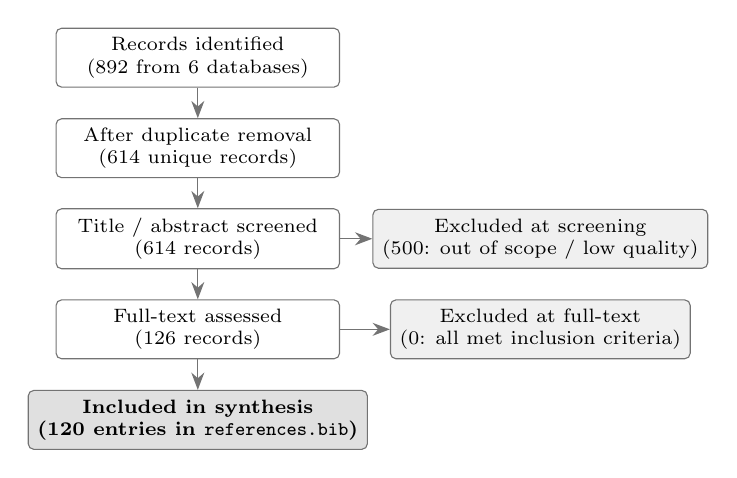
\begin{tikzpicture}[prisma/.style={draw=black!55, fill=white, rounded corners=2pt, minimum width=3.6cm, minimum height=0.72cm, align=center, font=\scriptsize}, prismaem/.style={prisma, fill=black!6, minimum width=3.0cm, minimum height=0.58cm}, arr/.style={-{Stealth[length=2.2mm]}, line width=0.45pt, draw=black!55}
]
  \node[prisma] (id) at (0,0) {Records identified\\(892 from 6 databases)};
  \node[prisma] (dedup) at (0,-1.15) {After duplicate removal\\(614 unique records)};
  \node[prisma] (screen) at (0,-2.3) {Title / abstract screened\\(614 records)};
  \node[prismaem] (excl1) at (4.35,-2.3) {Excluded at screening\\(500: out of scope / low quality)};
  \node[prisma] (full) at (0,-3.45) {Full-text assessed\\(126 records)};
  \node[prismaem] (excl2) at (4.35,-3.45) {Excluded at full-text\\(0: all met inclusion criteria)};
  \node[prisma, fill=black!12, font=\scriptsize\bfseries] (incl) at (0,-4.6)
    {Included in synthesis\\(120 entries in \texttt{references.bib})};
  \draw[arr] (id) -- (dedup);
  \draw[arr] (dedup) -- (screen);
  \draw[arr] (screen) -- (full);
  \draw[arr] (full) -- (incl);
  \draw[arr] (screen.east) -- (excl1.west);
  \draw[arr] (full.east) -- (excl2.west);
\end{tikzpicture}
\caption[PRISMA-style literature screening flow]{PRISMA-style literature screening flow}
\label{fig:prisma-flow}
\end{figure}

\begin{table}[H]
\centering
\footnotesize
\setlength{\tabcolsep}{4pt}
\renewcommand{\arraystretch}{1.12}
\caption[Top-10 ranked literature sources]{Top-10 ranked literature sources}
\label{tab:lit-top10}
\resizebox{\textwidth}{!}{%
\begin{tabular}{@{}cp{4.2cm}p{7.4cm}@{}}
\toprule
\tableheadcolor
\tableheadfont \# & \tableheadfont Source / Module / Operationalized In & \tableheadfont Headline Finding \\
\midrule
1 & Werner et al.\ 2022 [1] · DeFi mechanics · Ch.~3 & DeFi lending is uniformly flat, pool-based, overcollateralized \\
\rowcolor{RowShade}
2 & Tan 2023 (IMF) [5] · CBDC \& hierarchy · Ch.~3 & Two-tier CBDC distribution (central bank $\to$ commercial banks $\to$ users); hierarchical infrastructure is the key design choice \\
3 & Palaiokrassas et al.\ 2024 [3] · Fraud detection · Sec.~\ref{sec:aiml-support} & Multi-chain ML on 54M tx, F1 0.76--0.85 with behavioral features \\
\rowcolor{RowShade}
4 & Adom et al.\ 2022 [4] · Explainable AI · Sec.~\ref{sec:aiml-support} & SHAP outperforms LIME on lending datasets \\
5 & Weber et al.\ 2019 / Elliptic [85] · Graph fraud · Sec.~\ref{sec:gnn-extension} & Graph-structured fraud signal in BTC transactions \\
\rowcolor{RowShade}
6 & McMahan et al.\ 2017 / FedAvg [68] · Federated learning · Sec.~\ref{sec:fl-fraud} & Privacy-preserving model averaging across institutions \\
7 & BIS WP 905 [61] · Stablecoin risk · Secs.~\ref{sec:stablecoin-first}, \ref{sec:mica-compliance} & Algorithmic stablecoins unsuitable for EM DeFi; USDC/USDT recommended \\
\rowcolor{RowShade}
8 & Atzei et al.\ 2017 [7] · Smart contract security · Sec.~\ref{sec:defense-in-depth} & SoK of EVM attack vectors \\
9 & EU MiCA + GENIUS Act [75, 77] · Regulation · Sec.~\ref{sec:mica-compliance} & Stablecoin issuer authorization, reserve disclosure \\
\rowcolor{RowShade}
10 & Bangladesh Bank SP2025-02 [80] · MFI precedent · Sec.~\ref{sec:over-indebt} & Female-to-male account parity 49\%/49\% in 2025; 89\% BRAC loans to women \\
\bottomrule
\end{tabular}%
}
\end{table}

\section{Review of Existing Research}
\label{sec:review-existing}

This part of the paper explores all the literature chosen through a PRISMA-style screening flow to select the papers that best fit our project. We surveyed existing work related to DeFi lending, ML fraud detection and explainable AI, hierarchical development finance and cross-tier finance flows, group or microfinance, smart contracts and gas economics, retail banking and payments, remittance, monetary-policy distributional effects, real-world asset tokenization, stablecoin regulation and institutional settlement, and how inference can be achieved in systems like ours.

\subsection{Decentralized Lending and DeFi Protocol Design}

This is one of the most important parts of the paper: how decentralized financing works for lending, and how DeFi protocols are designed as public smart contracts. Utilization curves set interest rates; oracles trigger liquidations on collateral; settlement stays atomic across currencies. The model's real strength is real-time auditability---per-block interest and transparent on-chain state. It also comes with structural limits for development finance: capital still flows one way through flat pools, with no inter-tier allocation or multi-entity co-funding---a crucial gap for our project.

Werner et al.~[1] summarize DeFi as homogeneous, pool-based, and over-collateralized, with no institutional hierarchy. Bastankhah et al.~[2] show adaptive fast/slow rate control outperforming static Aave/Compound curves~[51], which informs our kinked-rate model (Section~\ref{sec:kinked-rate}). Chen et al.~[39] test multi-chain lending layouts to handle higher throughput. Yang and Cui~[40] propose practical metrics---utilization stability, liquidation efficiency, and rate responsiveness---for judging how well a lending stack performs. Hartmann and Hasan~[41] look at gas cost and digital identity in peer-to-peer lending. Dao et al.~[52] map traditional credit scoring onto DeFi borrowing limits.

\subsection{Machine Learning, Explainable AI, and Extended AI Security}

Palaiokrassas et al.~[3] achieve F1 0.76--0.85 on 54M multi-chain DeFi transactions using behavioral features versus 0.08 with raw transaction data alone---direct input to Random Forest feature engineering. Liu et al.~[6] supply Isolation Forest for unsupervised detection when labeled fraud is scarce. Hasan et al.~[42] train fraud classifiers via federated learning on encrypted features, informing cross-bank intelligence without raw data sharing.

Adom et al.~[4] find SHAP more consistent than LIME for loan explanations; Yuan~[49] reaches AUC $>$0.92 with SHAP on credit-default models---motivating SHAP waterfall review before approvals. Beyond the core pipeline, graph features from Palaiokrassas et al.~[3] support GNN ring detection; federated learning~[42] suits National/Local Bank boundaries; ContractWard~[43] and SoliAudit~[44] enable real-time exploit monitoring; RL rate tuning and NLP income extraction remain future-work options.

\subsection{Hierarchical Distribution, Cross-Tier Flows, and Group Lending}
\label{sec:lit-cross-tier}

Tan~[5] models two-tier CBDC distribution (central bank $\to$ commercial banks $\to$ users), paralleling the four-tier hierarchy. BIS~[46] prefers two-level retail CBDC with interoperability constraints, informing the dual-currency facility. Asaduzzaman et al.~[47] report up to 60\% admin-cost reduction from smart-contract microcredit---literature precedent for \texttt{GroupLendingPool}, not a deployment-jurisdiction claim.

Policy literature establishes hierarchical distribution but sparse programmable \emph{multi-directional} coordination. Kiff et al.~[106] distinguish multi-tier CBDC with supervised intermediaries; Bindseil~[105] analyses tiered remuneration for \texttt{UpwardDepositFacility} rate spreads (Section~\ref{sec:upward-flow}); Auer and B\"{o}hme~[107] hybrid CBDC mirrors client-via-Local-Bank access with Tier~1 reserve authority. \textit{Project Pine}~[103] validates layered contract factories for reserve and collateral dependencies extended by \texttt{InterBankLendingPool} and \texttt{SyndicatedLoan}. Dong et al.~[104] model cross-tier direct financing in supply chains---parallel to downward allocation to capital-constrained retail clients (Figure~\ref{fig:cross-tier-lending}).

Grameen/BRAC solidarity groups achieve $>$95\% repayment through social monitoring that on-chain mutual liability cannot fully replicate; \texttt{GroupLendingPool} encodes multi-signature consent and pool claims at pre-thesis stage. G\"{u}\c{c}\"uk et al.~[53] review privacy and trust in blockchain microlending.

\subsection{Smart Contract Security and Layer~2 Scalability}

Atzei et al.~[7] catalogue reentrancy, access-control, and overflow vectors---motivating OpenZeppelin guards, Solidity~0.8.20, RBAC, Slither, Mythril, and Phase~IV formal verification. Wang et al.~[43] (ContractWard) reach F1 0.96/0.93 on bytecode vulnerability classes; Liao et al.~[44] (SoliAudit) cut audit time $\approx$70\% via ML-prioritized fuzzing; So et al.~[45] (VERISMART) report 98.4\% precision with zero false positives on arithmetic safety---candidate for reserve-ratio invariants.

Transaction batching~[17] can save 15--59\% mainnet gas per call, with further DeFi gas optimisation~[48], supporting Polygon zkEVM Cardona deployment where multi-step four-tier lifecycles multiply savings.

\subsection{Correspondent Banking, Retail Payments, and Settlement Rails}
\label{sec:lit-retail-payments}

BIS~[16] and FSB~[27] document nostro/vostro idle capital, MT103 routing, and 2--5-day settlement. World Bank remittance data~[20] average 6.49\% on a \$200 transfer (Sub-Saharan Africa $>$8\%). Cerutti et al.~[116] and Du et al.~[110] show digital and stablecoin rails can undercut legacy costs but depend on corridor off-ramp depth---scoped separately (Section~\ref{sec:future-retail-payments}).

Retail literature examines stablecoin remittance, merchant checkout, and on/off-ramps for post-MVT modules (\texttt{CurrentAccount}, \texttt{P2PTransfer}). Ante~[108] finds 26\% U.S.\ remittance-user stablecoin adoption, supporting tiered KYC gating. Du et al.~[110] document the fiat--stablecoin--fiat ``sandwich'' pattern. Li et al.~[109] (\textbf{CLEAR} framework) find programmable settlement advantages but weak open-loop dispute recourse; Zhang et al.~[112] warn on refund volatility; Fr\"{o}hlich et al.~[111] show on-ramp friction dominates POS UX. Lin et al.~[113] (\textit{SecurePay}) and BIS \textit{Project Sela}~[119] validate Local-Bank--sponsored multi-intermediary flows; Cimaszewski et al.~[118] blueprint jurisdictional DLT settlement. CPMI~[114], BIS Papers~170~[115], and FATF~[117] define ramp and VASP compliance for platform-mediated \texttt{P2PTransfer}---not permissionless unhosted-wallet remittance. No prior work composes four-tier development-finance lending with closed-loop retail rails in one architecture.

\subsection{Monetary Policy, Tokenization, and Institutional Landscape}
\label{sec:lit-institutional}

Cross-country evidence links QE to wealth inequality~[28]; Federal Reserve metro analysis~[29] shows low-income harm from tightening---motivating algorithmic, transparent rate and reserve parameters rather than opaque committee discretion. Tier-uniform utilization rates reduce loan-officer price discrimination; the Cantillon effect does not apply where USDC is fully reserved and the platform creates no new money~[30].

R3 Corda reports \$17B tokenized RWAs~[31]; Centrifuge exceeds \$1B across eight chains~[32]; World Bank FundsChain tracks disbursements on 13 projects scaling to 250~[33]---institutional precedent for hierarchical on-chain finance beyond fund tracking alone.

Sygnum~[65] notes institutional allocators require legal enforceability (Aave Arc $\approx$\$50k TVL). mBridge~[78] and \textit{Project Agora}~[79] are settlement rails, not retail lending hierarchies; 94\% of central banks research CBDCs~[71]. CWB positions as a lending-layer specification compatible with these rails.

\subsection{Graph ML, Federated Learning, Regulation, and Identity Primitives}

DeFi fraud is relational: Cheng et al.~[93], Chang et al.~[93], and DeFiGuard~[67] outperform flat ML on graph structure---motivating a GNN extension with hierarchical tier edges (Section~\ref{sec:gnn-extension}). Federated learning~[42, 97] and PrivChain-AI (94.7\% accuracy) suit banks that cannot share raw records; FedAvg aggregation at National tier is architecturally natural (Section~\ref{sec:fl-fraud}).

MiCA~[75, 76] and the U.S.\ GENIUS Act~[77] anchor stablecoin-first retail design (Section~\ref{sec:stablecoin-first}; mapping in Section~\ref{sec:mica-compliance}). Buterin et al.~[69] introduce non-transferable SBTs for portable credit passports~[70] (Section~\ref{sec:credit-passport}).

\subsection{Oracle-Mediated ML and Optional LLM Interfaces}
\label{sec:lit-llm}

Luo et al.~[94] survey AI fraud detection across the DeFi lifecycle; Caldarelli~[95] identifies ML-score oracle delivery as under-researched beyond price feeds. BCCC-DeFiFraudTrans-2025~[83] (1,026,867 labeled transactions) is the planned primary training corpus after pre-thesis 2 (Section~\ref{sec:ml-workload}); Fazliani et al.~[96] and Alhasawi et al.~[97] supply semi-supervised and federated baselines.

The optional conversational add-on uses an 8B open-weight LLM with QLoRA, RAG, and refusal layers. Finance LLM studies~[72, 73, 74] report productivity gains but document regulatory-hallucination risks---motivating the red-team protocol in Section~\ref{sec:llm-eval}.

\section{Literature Review Summary}

Tables~\ref{tab:lit-summary} and~\ref{tab:lit-summary-b} consolidate the reviewed works by methodology, findings, and project relevance. Extended six-part synthesis tables are maintained in the thesis repository.

\begin{table}[H]
\centering
\footnotesize
\setlength{\tabcolsep}{3pt}
\renewcommand{\arraystretch}{1.08}
\caption[Literature review summary (Part 1 of 2)]{Literature review summary (Part 1 of 2)}
\label{tab:lit-summary}
\resizebox{\textwidth}{!}{%
\begin{tabular}{@{}>{\raggedright\arraybackslash}p{3.0cm}>{\raggedright\arraybackslash}p{2.6cm}>{\raggedright\arraybackslash}p{3.4cm}>{\raggedright\arraybackslash}p{3.2cm}@{}}
\toprule
\tableheadcolor
\tableheadfont Author \& Focus & \tableheadfont Methodology & \tableheadfont Key Findings & \tableheadfont Relevance to Our Project \\
\midrule
Palaiokrassas et al.\ (2024) [3] · DeFi fraud & XGBoost, NN on 54M+ txs & F1: 0.76--0.85 vs.\ 0.08 with features alone & Random Forest fraud modeling \\
Adom et al.\ (2022) [4] · XAI lending & LIME / SHAP comparison & SHAP deeper, more consistent than LIME & Primary explainability method \\
Tan (2023) [5] · CBDC hierarchy & Developing-nation model & Two-tier CBDC distribution; hierarchy decisive & Four-tier architecture \\
Liu et al.\ (2008) [6] · Anomaly detection & Isolation Forest & Recursive partitioning; shorter paths & Unsupervised wallet detection \\
Atzei et al.\ (2017) [7] · SC security & SoK of Ethereum attacks & Reentrancy, access-control gaps & Security primitives, formal verification \\
Werner et al.\ (2022) [1] · DeFi SoK & Survey of 12+ protocol types & Pool-based, overcollateralised; no hierarchy & Core gap CWB addresses \\
Bastankhah et al.\ (2024) [2] · Adaptive lending & Dual fast/slow control & Dynamic rates beat static curves & Kinked-rate validation \\
Hartmann \& Hasan (2021) [41] · P2P lending & Smart-contract origination & Gas minimisation; no intermediary & Four-tier P2P design \\
Hasan et al.\ (2022) [42] · Federated fraud & FL on encrypted features & Comparable to centralised ML & Cross-bank intelligence \\
Wang et al.\ (2020) [43] · SC vulnerabilities & ML on bytecode & F1: 0.96 access control; 0.93 leakage & Security verification models \\
Liao et al.\ (2019) [44] · Audit automation & Classification + fuzzing & 70\% faster than manual audit & Security audit strategy \\
\bottomrule
\end{tabular}%
}
\TableScreenshotEnd{Literature Review Summary (Part 1 of 2): DeFi, ML, and Security}
\end{table}

\begin{table}[H]
\centering
\footnotesize
\setlength{\tabcolsep}{3pt}
\renewcommand{\arraystretch}{1.08}
\caption[Literature review summary (Part 2 of 2)]{Literature review summary (Part 2 of 2)}
\label{tab:lit-summary-b}
\resizebox{\textwidth}{!}{%
\begin{tabular}{@{}>{\raggedright\arraybackslash}p{3.0cm}>{\raggedright\arraybackslash}p{2.6cm}>{\raggedright\arraybackslash}p{3.4cm}>{\raggedright\arraybackslash}p{3.2cm}@{}}
\toprule
\tableheadcolor
\tableheadfont Author \& Focus & \tableheadfont Methodology & \tableheadfont Key Findings & \tableheadfont Relevance to Our Project \\
\midrule
BIS et al.\ (2020) [46] · CBDC design & Retail distribution analysis & Two-tier preferred; interoperability gaps & Dual-currency facility \\
Kiff et al.\ (2020) [106] · CBDC models & IMF architecture survey & Multi-tier via supervised intermediaries & Wholesale-to-retail path \\
Bindseil (2020) [105] · CBDC rates & ECB tiered remuneration & Preserves bank intermediation & Asymmetric rate spread \\
Dong et al.\ (2023) [104] · Supply-chain finance & Three-tier game model & Cross-tier direct financing & Downward client lending \\
Project Pine (2025) [103] · Hierarchical SCs & NY Fed / BIS prototype & Factory-to-facility hierarchy & \texttt{IBLP} / \texttt{SyndicatedLoan} \\
CPMI/FSB [18, 27] · Cross-border settlement & Nostro/vostro cost analysis & 2--5 days; \$45/transfer avg. & Near-instant four-tier settlement \\
Beyer et al.\ (2025) [28] · QE inequality & Cross-country 1999--2019 & QE raises wealth inequality & Algorithmic monetary parameters \\
World Bank (2025) [33] · Dev.\ finance blockchain & 13-project pilot & Reduces reporting burden & Multi-chain deployment \\
Chen et al.\ (2024) [39] · Multi-chain lending & Cross-chain design & Higher throughput, less congestion & Multi-chain strategy \\
Yang \& Cui (2023) [40] · Protocol evaluation & Quantitative risk metrics & Utilisation, liquidation, responsiveness & Tier benchmarks \\
Asaduzzaman et al.\ (2020) [47] · Smart micro-credit & Smart-contract MFI & 60\% admin overhead reduction & \texttt{GroupLendingPool} \\
Wang et al.\ (2021) [17] · Tx batching & iBatch middleware & 15--59\% gas savings per call & L2 deployment \\
Kim \& Kim (2024) [48] · Gas optimisation & DeFi parameter tuning & $\sim$18\% gas cut on Ethereum pools & Complements L2 deployment \\
Yuan (2024) [49] · SHAP credit default & RF, GBM + SHAP & AUC $>$0.92, interpretable & Per-client risk explanation \\
\bottomrule
\end{tabular}%
}
\TableScreenshotEnd{Literature Review Summary (Part 2 of 2): Hierarchy, Institutions, and Retail Rails}
\end{table}

\newpage
\begin{table}[H]
\centering
\footnotesize
\setlength{\tabcolsep}{3pt}
\renewcommand{\arraystretch}{1.08}
\caption[]{Literature review summary (Part 2 of 2, continued)}
\resizebox{\textwidth}{!}{%
\begin{tabular}{@{}>{\raggedright\arraybackslash}p{3.0cm}>{\raggedright\arraybackslash}p{2.6cm}>{\raggedright\arraybackslash}p{3.4cm}>{\raggedright\arraybackslash}p{3.2cm}@{}}
\toprule
\tableheadcolor
\tableheadfont Author \& Focus & \tableheadfont Methodology & \tableheadfont Key Findings & \tableheadfont Relevance to Our Project \\
\midrule
Ante (2025) [108] · Stablecoin remittance & U.S.\ survey ($n{=}866$) & 26\% adoption; literacy drives uptake & KYC ladder, \texttt{P2PTransfer} \\
Du et al.\ (2026) [110] · Payment rails & Corridor cost comparison & Stablecoin sandwich undercuts banks & PSP on/off-ramp work \\
Li et al.\ (2026) [109] · Retail payments SoK & CLEAR framework & Closed-loop advantage; weak disputes & Merchant checkout design \\
Zhang et al.\ (2024) [112] · Stablecoin checkout & Operations model & Refund volatility disutility & \texttt{FXModule}, auto-conversion \\
Fr\"{o}hlich et al.\ (2022) [111] · Crypto POS & Lightning usability & On-ramp friction dominates & Fiat-funded \texttt{CurrentAccount} \\
Lin et al.\ (2025) [113] · Platform payments & Permissioned chain prototype & $\approx$256~TPS; multi-intermediary escrow & Local-Bank merchant flows \\
CPMI / BIS [114, 115] · Stablecoin policy & Cross-border analysis & Ramps gate acceptance & Ramp integration \\
FATF (2021) [117] · VASP / P2P & Risk-based AML & Platform transfers need originator data & Sponsored \texttt{P2PTransfer} \\
\bottomrule
\end{tabular}%
}
\end{table}

\section{Comparative Protocol Analysis}
\label{sec:comparative-protocol}

No surveyed protocol combines multi-tier hierarchy, oracle-mediated explainable ML, and compliance-aware identity. Table~\ref{tab:protocol-comparison} compares CWB against Aave, Compound, Maker, Maple, and Goldfinch on eleven architectural dimensions.

\begin{table}[H]
\centering
\footnotesize
\setlength{\tabcolsep}{3pt}
\resizebox{\textwidth}{!}{%
\begin{tabular}{@{}p{3.4cm}*{6}{>{\centering\arraybackslash}p{1.35cm}}@{}}
\toprule
\tableheadcolor
\tableheadfont Feature & \tableheadfont Aave & \tableheadfont Comp. & \tableheadfont Maker & \tableheadfont Maple & \tableheadfont Gfinch & \tableheadfont CWB \\
\midrule
Institutional hierarchy & \tmarkNo{} & \tmarkNo{} & \tmarkNo{} & \tmarkNo{} & \tmarkNo{} & \tmarkPlanned{} \\
\rowcolor{RowShade}
Cross-tier capital flow & \tmarkNo{} & \tmarkNo{} & \tmarkNo{} & \tmarkNo{} & \tmarkNo{} & \tmarkPartial{} \\
Same-tier interbank lending & \tmarkNo{} & \tmarkNo{} & \tmarkNo{} & \tmarkNo{} & \tmarkNo{} & \tmarkPartial{} \\
\rowcolor{RowShade}
Syndicated / co-lending & \tmarkNo{} & \tmarkNo{} & \tmarkNo{} & Part. & Part. & \tmarkPartial{} \\
Upward capital repatriation & \tmarkNo{} & \tmarkNo{} & \tmarkNo{} & \tmarkNo{} & \tmarkNo{} & \tmarkPartial{} \\
\rowcolor{RowShade}
Solidarity group lending & \tmarkNo{} & \tmarkNo{} & \tmarkNo{} & \tmarkNo{} & Part. & \tmarkPlanned{} \\
AI/ML fraud detection & \tmarkNo{} & \tmarkNo{} & \tmarkNo{} & Man. & Man. & \tmarkPlanned{} \\
\rowcolor{RowShade}
SHAP explainability & \tmarkNo{} & \tmarkNo{} & \tmarkNo{} & \tmarkNo{} & \tmarkNo{} & \tmarkPlanned{} \\
ZKP KYC compliance & \tmarkNo{} & \tmarkNo{} & \tmarkNo{} & \tmarkNo{} & \tmarkNo{} & \tmarkPlanned{} \\
\rowcolor{RowShade}
Kinked interest rate curve & \tmarkDone{} & \tmarkDone{} & Gov. & \tmarkDone{} & \tmarkNo{} & \tmarkPartial{} \\
Role-based access control & Part. & Part. & Gov. & \tmarkDone{} & Part. & \tmarkPlanned{} \\
\rowcolor{RowShade}
Institutional / L2 focus & \tmarkNo{} & \tmarkNo{} & \tmarkNo{} & \tmarkDone{} & Part. & \tmarkPlanned{} \\
TVL / Status (2026) & \$26B & \$1.4B & \$10B & \$2.6B & \$680M & Planning \\
\bottomrule
\end{tabular}%
}
\caption[Protocol comparison on eleven architectural dimensions]{Protocol comparison on eleven architectural dimensions}
\label{tab:protocol-comparison}
\end{table}

This answers RQ1: flat-pool protocols differentiate assets, not institutional relationships or inter-bank flows; Maple, Goldfinch, and Morpho~V2~[117, 90] lack multilateral development-finance capital allocation. CWB's compound novelty (Section~\ref{sec:research-contribution}) spans hierarchy, explainable ML governance, and group lending. Tiers~1--3 use bespoke RBAC (Section~\ref{sec:defense-in-depth}) functionally equivalent to ERC-3643 token-level KYC gating~[82]; enforced per-tier reserve ratios address opaque custody failures such as FTX's 2022 collapse.

Six design decisions follow from the survey:
\begin{itemize}[noitemsep]
\item Gudgeon et al.~[56] $\to$ kinked-rate model (Section~\ref{sec:kinked-rate})
\item Piper et al.~[58] $\to$ ZKP identity path (Section~\ref{sec:identity})
\item Tan~[5], BIS~[46], Kiff~[106], Auer and B\"{o}hme~[107] $\to$ four-tier capital flows
\item Bindseil~[105], Project Pine~[103], Dong et al.~[104] $\to$ multi-directional lending (Section~\ref{sec:cross-tier-lending})
\item Asaduzzaman et al.~[47] $\to$ \texttt{GroupLendingPool}
\item Ante~[108], Du et al.~[110], Li et al.~[109], Lin et al.~[113], CPMI~[114], FATF~[117] $\to$ post-MVT retail stack (Section~\ref{sec:future-retail-payments})
\end{itemize}

\section{Summary of Key Findings}
\label{sec:lit-key-findings}

The literature review yields the following design-relevant conclusions:

\begin{itemize}[noitemsep]
\item \textbf{Flat DeFi vs.\ tiered finance.} Pool-based protocols exceed \$55B TVL~[8] but lack institutional hierarchy; CBDC research confirms tiered distribution as a workable pattern~[5]. No prior work models four-tier reserve-enforced lending.
\item \textbf{Settlement and retail rails.} Correspondent banking traps idle capital~[18], settles in 2--5 days at $\approx$\$45/transfer~[19], and costs remittance users \$48--56B annually~[20]. Stablecoin rails can compress costs~[116, 110] but need ramp infrastructure; retail studies~[109, 112, 111, 113, 119] favour Local-Bank--sponsored closed-loop flows over open permissionless checkout.
\item \textbf{ML, XAI, and security.} Behavioral DeFi features lift fraud F1 to 0.76--0.85~[3]; Isolation Forest~[6] covers unlabeled cases; SHAP beats LIME for regulatory explainability~[4]. Contract vulnerabilities are well catalogued~[7]; ML audit tools reach F1 $>$0.93~[43], cut review time 70\%~[44], and formal verifiers such as VERISMART reach 98.4\% precision~[45].
\item \textbf{Hierarchy, groups, and institutions.} Cross-tier CBDC and Project Pine literature~[106, 105, 107, 103, 104] supports multi-directional programmable flows; analogue MFIs report $>$95\% group repayment~[47] with on-chain mutual liability still an open gap. FundsChain~[33], Corda RWAs~[31], and Kinexys~[34] show rising institutional blockchain adoption.
\item \textbf{Scalability, privacy, and regulation.} Multi-chain lending~[39] and L2 gas batching~[17, 48] cut costs 15--59\%; federated learning~[42, 97] enables cross-bank fraud intelligence without raw data sharing. MiCA and GENIUS~[75, 77] anchor stablecoin-first design; algorithmic parameters mitigate distributional opacity from discretionary monetary policy~[28, 29].
\item \textbf{Deposit-funded sustainability.} Sustainable MFIs rely on mobilized deposits, not donor capital alone---motivating savings vaults at the Local Bank tier alongside \texttt{GroupLendingPool}.
\end{itemize}

These findings justify the four-tier architecture, cross-tier lending modules, Random Forest / Isolation Forest / SHAP analytics, governance structure, and phased security verification pipeline developed in later chapters.

%% CHAPTER 3: SYSTEM ARCHITECTURE AND DESIGN
\chapter{System Architecture and Design}

\section{Prototype Scope}
\label{sec:prototype-scope}

\begin{table}[H]
\centering
\caption[Prototype scope and implementation status]{Prototype scope and implementation status}
\label{tab:prototype-scope}
\footnotesize
\renewcommand{\arraystretch}{0.88}
\setlength{\tabcolsep}{3pt}
\begin{tabular}{@{}p{7.1cm}>{\raggedleft\arraybackslash}p{5.9cm}@{}}
\toprule
\tableheadcolor
\tableheadfont Feature & \tableheadfont Status \\
\midrule
Four-tier role system (RBAC) & \tmarkPartial{} Specified \\
\rowcolor{RowShade}
World Bank Reserve contract (Tier~1) & \tmarkPartial{} Specified (Phase~I) \\
Tier~2 National Bank contracts & \tmarkPartial{} Specified (Phase~I) \\
\rowcolor{RowShade}
Tier~3 Local Bank contracts & \tmarkPartial{} Specified (Phase~I) \\
Cross-tier fund transfer & \tmarkPlanned{} Planned (Phase~II) \\
\rowcolor{RowShade}
Loan request / approval workflow & \tmarkPartial{} Specified (Phase~II) \\
Installment EMI auto-generation & \tmarkPlanned{} Planned (Phase~II) \\
\rowcolor{RowShade}
SavingsVault contract & \tmarkPlanned{} Planned (Phase~II) \\
FixedDeposit contract & \tmarkPlanned{} Planned (Phase~II) \\
\rowcolor{RowShade}
GroupLendingPool contract & \tmarkPlanned{} Planned (Phase~II) \\
InterBankLendingPool & \tmarkPlanned{} Planned (Phase~II) \\
\rowcolor{RowShade}
AI/ML fraud detection (Random Forest) & \tmarkPlanned{} Planned (Phase~III) \\
SHAP + anomaly explainability & \tmarkPlanned{} Planned (Phase~III) \\
\rowcolor{RowShade}
Oracle integration (Chainlink Functions) & \tmarkPlanned{} Planned (Phase~III) \\
ZKP KYC compliance layer & \tmarkPlanned{} Planned (Phase~IV) \\
\rowcolor{RowShade}
Testnet deployment (Polygon zkEVM Cardona) & \tmarkPlanned{} Planned (Phase~IV) \\
AI Agent / MCP tool server (17 tools) & \tmarkPlanned{} Optional (Phase~III--IV) \\
\rowcolor{RowShade}
EIP-7702 session key management & \tmarkPlanned{} Optional (Phase~III) \\
Authority Brief UI (SHAP for approvers) & \tmarkPlanned{} Planned (Phase~III) \\
\rowcolor{RowShade}
Chainlink Automation (installment triggers) & \tmarkPlanned{} Planned (Phase~II) \\
Chainlink Proof of Reserve & \tmarkPlanned{} Planned (Phase~I) \\
\rowcolor{RowShade}
The Graph subgraph (event indexing) & \tmarkPlanned{} Planned (Phase~III) \\
SAR workflow (AML $\to$ freeze queue) & \tmarkPlanned{} Planned (Phase~III) \\
\rowcolor{RowShade}
\texttt{sessions} table schema & \tmarkPartial{} Specified (Phase~I) \\
\texttt{agent\_action\_log} table schema & \tmarkPlanned{} Optional (Phase~III) \\
\rowcolor{RowShade}
300-client Foundry simulation & \tmarkPlanned{} Planned (Phase~IV) \\
\bottomrule
\end{tabular}
\end{table}

\section{High-Level Architecture}
\label{sec:high-level-arch}

\begin{figure}[H]
\centering
\BalancedDiagram{fig-three-layer-arch.pdf}
\caption[Four-layer application architecture]{Four-layer application architecture}
\label{fig:three-layer-arch}
\end{figure}

Figure~\ref{fig:component-diagram} shows component interactions. Core lending contracts are specified in Phase~I; extended modules are planned extensions documented in Appendix~B.

\begin{figure}[H]
\centering
\BalancedDiagram{fig-component-architecture.pdf}
\caption[Component diagram (planning phase)]{Component diagram (planning phase)}
\label{fig:component-diagram}
\end{figure}

\begin{table}[H]
\centering
\begin{tabular}{p{3.6cm}p{2.4cm}p{1.8cm}p{6.7cm}}
\toprule
\tableheadcolor
\textbf{Contract} & \textbf{Module} & \textbf{Status} & \textbf{Primary responsibility} \\
\midrule
WorldBankReserve & Tier~1 core & Specified (Phase~I) & Global reserve custody, national-bank registration, downward capital allocation. \\
NationalBank & Tier~2 core & Specified (Phase~I) & Local-bank registration, upward borrowing, downward allocation. \\
LocalBank & Tier~3 core & Specified (Phase~I) & Client onboarding, loan lifecycle, installments, \texttt{freezeAccount}. \\
SavingsVault & Deposits & Specified (Phase~II) & Variable-yield savings, reserve-gated withdrawals. \\
FixedDeposit & Deposits & Specified (Phase~II) & Term deposits with deterministic early-withdrawal penalty. \\
GroupLendingPool & Group credit & Specified (Phase~II) & Solidarity-group formation, consent, mutual liability. \\
FXModule & Treasury / FX & Specified (Phase~II) & Oracle-priced retail FX with disclosed spread. \\
InsuranceFund & Risk buffer & Specified (Phase~II) & Default coverage buffer; Chainlink Proof of Reserve. \\
CurrentAccount & Payments & Specified (Phase~II) & Transactional accounts and atomic peer transfers. \\
InterBankLendingPool & Multi-entity & Specified (Phase~II) & Same-tier interbank liquidity pools per tier. \\
UpwardDepositFacility & Multi-entity & Specified (Phase~II) & Upward surplus repatriation with yield spread. \\
SyndicatedLoan & Multi-entity & Planned (Phase~III) & Multi-lender syndicate consent and disbursement. \\
TranchedPool & Multi-entity & Planned (Phase~III) & Senior/junior tranching and waterfall recovery. \\
TreasurySwap & Multi-entity & Specified (Phase~II) & Institutional oracle-priced asset swaps. \\
NettingEngine & Multi-entity & Planned (Phase~III) & Multilateral settlement netting batches. \\
\bottomrule
\end{tabular}
\TableScreenshotEnd{Smart Contract Inventory: Fifteen Modular Contracts Across Core, Product, and Multi-Entity Modules}
\end{table}

\section{Blockchain Platform Selection}

\begin{figure}[H]
\centering
\BalancedDiagram{fig-blockchain-stack.pdf}
\caption[Layered blockchain and application stack]{Layered blockchain and application stack}
\label{fig:blockchain-stack}
\end{figure}

\begin{table}[H]
\centering
\caption[Blockchain platform selection criteria and justification]{Blockchain platform selection criteria and justification}
\label{tab:blockchain-selection}
\begin{tabular}{p{3.5cm}p{3.5cm}p{6.5cm}}
\toprule
\tableheadcolor
\textbf{Criterion} & \textbf{Selection} & \textbf{Justification} \\
\midrule
Platform & Ethereum Virtual Machine (EVM) & Largest developer ecosystem; battle-tested security model; extensive tooling. \\
Network & Polygon zkEVM Cardona / Ethereum Sepolia & Zero-cost deployment; production-equivalent behaviour; free faucet access. \\
Consensus & ZK validity proofs (Polygon zkEVM L2, Ethereum L1 settlement) & Every batch of transactions is accompanied by a zero-knowledge proof verified on Ethereum L1, so security derives from cryptographic validity rather than a validator set assumption. \\
Smart contract language & Solidity 0.8.20 & Industry standard; mature compiler with overflow protection; rich library ecosystem. \\
\bottomrule
\end{tabular}
\TableScreenshotEnd{Blockchain Platform Selection: Comparison of EVM-Compatible Networks}
\end{table}

\vspace{2pt}

\begin{table}[H]
\centering
\caption[Blockchain platform selection (continued)]{Blockchain platform selection (continued)}
\begin{tabular}{p{3.5cm}p{3.5cm}p{6.5cm}}
\toprule
\tableheadcolor
\textbf{Criterion} & \textbf{Selection} & \textbf{Justification} \\
\midrule
Gas cost & \$0.001--\$0.01 per transaction & Orders of magnitude cheaper than Ethereum mainnet (\$5--\$50); enables micro-loan economics. \\
Block finality & $\approx$2 seconds & Sub-second practical finality for retail UX; checkpointed to Ethereum for security. \\
Developer tooling & Hardhat + OpenZeppelin & Automated test suite, deployment scripts, and audited security primitives. \\
Testnet availability & Cardona (Polygon zkEVM), Sepolia (Ethereum) & Free faucets; EVM-identical behaviour; no real cryptocurrency required for prototype. \\
Security model & ZK validity proofs & Every batch verified by a ZK proof anchored to Ethereum L1 (vs.\ PoS validator assumption on Amoy). \\
Migration path & EVM-compatible & Same Solidity contracts deploy to any EVM chain; reduces future L2 migration cost. \\
\bottomrule
\end{tabular}
\TableScreenshotEnd{Blockchain Platform Selection (Continued): Operational and Deployment Factors}
\end{table}

\vspace{2pt}

\subsection{Transaction Verification and Consensus}

\begin{itemize}[noitemsep]
\item \textbf{Polygon zkEVM Cardona:} ZK validity proofs anchor batches to Ethereum~L1 (cryptographic security vs.\ PoS validator assumption on Amoy).
\item \textbf{On prototype testnets:} Cardona and Sepolia use equivalent consensus models at no financial cost, enabling incremental development and testing without exposure to real-asset risk.
\end{itemize}

\paragraph{Gas-cost sustainability.}
The hierarchical loan lifecycle generates multiple on-chain state transitions per client; on Polygon zkEVM Cardona the \textbf{projected} cost remains well below 0.01\% of interest earned on a representative retail loan (Section~\ref{sec:gas-cost}), to be validated by the Phase~IV Foundry simulation. This margin underpins the micro-loan economics that motivate Layer~2 deployment in the platform selection above.

\subsection{Oracle Architecture: Off-Chain AI to On-Chain Decision}
\label{sec:oracle-architecture}

Contracts cannot read ML scores on their own---the classic oracle problem~[55, 95]. Publishing non-price ML output on-chain is still thinly studied~[95]. CWB pipes off-chain risk into loan approval via Chainlink~[122--124], with a lighter commit-reveal relay for early prototyping~[125].

\paragraph{Chainlink Functions oracle (primary).}
\textbf{Chainlink Functions}~[122] is the target path: DON nodes fetch the score independently and only commit after consensus~[55], so one bad node cannot move a decision. The DON runs:

\begin{verbatim}
// Chainlink Functions source (runs in decentralised DON)
const clientId = args[0];
const response = await Functions.makeHttpRequest({
 url: `https://your-ml-service.com/score/${clientId}`,
 method: "POST"
});
const score = response.data.risk_score;
// 6 decimal precision
return Functions.encodeUint256(Math.round(score * 1e6));
\end{verbatim}

Expect 30--60\,s latency and roughly \$0.10--\$1.00 per call~[122]---fine for loan approval, which is not latency-critical.

\paragraph{Commit-reveal relay (prototype fallback).}
Until Functions is wired (Phase~III), FastAPI commits $h = \text{keccak256}(s \,\|\, \text{nonce})$ to \texttt{LoanController}, then reveals $s$ and the nonce in-window---the standard commit-reveal pattern~[125]. The contract checks the hash and stores the score.

\paragraph{Chainlink Automation: trustless installment triggers.}
\textbf{Chainlink Automation}~[123] flags overdue installments without a central cron; \texttt{checkUpkeep}/\texttt{performUpkeep} follow the keeper interface~[123]:

\begin{verbatim}
// In LocalBankPool.sol
function checkUpkeep(bytes calldata) external view override
 returns (bool upkeepNeeded, bytes memory performData) {
 uint256[] memory overdueLoans = getOverdueLoans;
 upkeepNeeded = overdueLoans.length > 0;
 performData = abi.encode(overdueLoans);
}

function performUpkeep(bytes calldata performData) external override {
 uint256[] memory overdueLoans =
 abi.decode(performData, (uint256[]));
 for (uint i = 0; i < overdueLoans.length; i++) {
 _markInstallmentOverdue(overdueLoans[i]);
 }
}
\end{verbatim}

\paragraph{Chainlink Price Feeds: fiat and crypto pairs.}
\texttt{FXModule} reads \texttt{AggregatorV3Interface} feeds (ETH/USD, USDC/USD, selected fiat pairs)~[124]:

\begin{verbatim}
// In LocalBankPool.sol
AggregatorV3Interface internal fiatUsdFeed; // e.g. EUR/USD
AggregatorV3Interface internal ethUsdFeed;

function getFiatEquivalent(uint256 usdcAmount)
 public view returns (uint256) {
 (, int fiatRate,,,) = fiatUsdFeed.latestRoundData;
 // USDC tracks USD 1:1; Chainlink uses 8 decimals
 return usdcAmount * uint256(fiatRate) / 1e8;
}
\end{verbatim}

Chainlink's 8-decimal feed format~[124]; Phase~I adds optional fiat display in the UI.

\paragraph{Chainlink Proof of Reserve.}
\texttt{WorldBankReserve} can publish to \textbf{Chainlink Proof of Reserve (PoR)}~[103] so outsiders verify solvency without trusting the admin:

\begin{verbatim}
// WorldBankReserve.sol
function getReserveSummary external view returns (
 uint256 totalDeposited,
 uint256 totalLoaned,
 uint256 reserveRatio, // scaled 1e4 (e.g. 5000 = 50%)
 uint256 insuranceFundBalance
) {
 return (
 totalDeposited,
 totalLoaned,
 (totalDeposited - totalLoaned) * 1e4 / totalDeposited,
 insuranceFund.balance
 );
}
\end{verbatim}

Same reserve logic as Section~\ref{sec:defense-in-depth}; PoR makes it externally auditable (Appendix~D).

\begin{figure}[H]
\centering
\BalancedDiagram{fig-oracle-architecture.pdf}
\caption[Chainlink oracle architecture]{Chainlink oracle architecture}
\label{fig:oracle-architecture}
\end{figure}

\section{Data Model and Database Design}
\label{sec:data-model}

The relational database schema comprises 20 normalized entities in Third Normal Form (3NF). Figure~\ref{fig:core-system-graph} presents the core entity-relationship overview, Figure~\ref{fig:erd-extended} presents extended product and multi-entity entities, and Figure~\ref{fig:eer} presents the Enhanced Entity-Relationship (EER) diagram with specialisation and weak-entity constructs.

\begin{figure}[H]
\centering
\BalancedDiagram{fig-erd-core.pdf}
\caption[Core system entity graph]{Core system entity graph}
\label{fig:core-system-graph}
\end{figure}

\begin{figure}[H]
\centering
\BalancedDiagram{fig-erd-extended.pdf}
\caption[Extended ERD entities]{Extended ERD entities}
\label{fig:erd-extended}
\end{figure}

Figure~\ref{fig:erd-extended} adds the remaining product and cross-tier tables on top of the core model. Full relationship detail is in Section~\ref{sec:multi-entity}; the schema matches the contract layout in the phase plan.

\begin{figure}[H]
\centering
\BalancedDiagram{fig-eer-model.pdf}
\caption[Enhanced EER model]{Enhanced EER model}
\label{fig:eer}
\end{figure}

\clearpage
\subsection{Entity Summary}

\begin{table}[H]
\centering
\caption[Database entity summary (20 entities)]{Database entity summary (20 entities)}
\label{tab:db-entities}
\small
\begin{tabular}{@{}p{2.6cm}p{3.4cm}p{7.0cm}@{}}
\toprule
\tableheadcolor
\textbf{Entity} & \textbf{Primary key} & \textbf{Role / Description} \\
\midrule
WORLD\_BANK & \texttt{world\_bank\_id} & Top-level reserve holder; global lending parameters. \\
NATIONAL\_BANK & \texttt{national\_bank\_id} & Country-level banks; borrow from World Bank. \\
LOCAL\_BANK & \texttt{local\_bank\_id} & City-level banks; borrow from National Bank and lend to users. \\
BANK\_USER & \texttt{bank\_user\_id} & Bank staff with role-based permissions (approve/reject loans). \\
BORROWER (CLIENT) & \texttt{borrower\_id} & End clients requesting and repaying loans (UK: \texttt{wallet\_address}). Renamed \texttt{CLIENT} in the final migration; prototype retains \texttt{BORROWER}. \\
LOAN\_REQUEST & \texttt{request\_id} & Loan applications and approval workflow tracking. \\
LOAN & \texttt{loan\_id} & Active loan after disbursement; FK \texttt{loan\_request\_id} $\to$ \texttt{LOAN\_REQUEST}; collateral and loan asset references. \\
INSTALLMENT & \texttt{loan\_id}, \texttt{installment\_number} & Repayment schedule (weak entity on \texttt{LOAN}; composite PK). \\
TRANSACTION & \texttt{transaction\_id} & Financial transaction records. \\
BORROWING\_LIMIT & \texttt{limit\_id} & Per-client limits with 6-month and 1-year rolling windows (UK: \texttt{borrower\_id}). \\
\bottomrule
\end{tabular}
\TableScreenshotEnd{Database Entity Summary (Part A): Core Lending and Client Entities}
\end{table}

\newpage
\begin{table}[H]
\centering
\caption[Database entity summary (continued)]{Database entity summary (continued)}
\small
\begin{tabular}{@{}p{2.6cm}p{3.4cm}p{7.0cm}@{}}
\toprule
\tableheadcolor
\textbf{Entity} & \textbf{Primary key} & \textbf{Role / Description} \\
\midrule
INCOME\_PROOF & \texttt{proof\_id} & Income verification documents (multi-valued per client). \\
CHAT\_MESSAGE & \texttt{message\_id} & Client--bank communication; FK to \texttt{LOAN\_REQUEST} and/or \texttt{LOAN}. \\
AI\_CHATBOT\_LOG & \texttt{log\_id} & AI chatbot interaction records. \\
AI\_ML\_SECURITY & \texttt{security\_log\_id} & Two logically distinct domains aggregated for the prototype: (1)~\texttt{LOAN\_RISK\_ASSESSMENT} per-loan scores and SHAP vectors; (2)~\texttt{SECURITY\_EVENT\_LOG} for system-wide events. Final thesis splits into separate tables. \\
MARKET\_DATA & \texttt{market\_data\_id} & Cryptocurrency price feed cache (Express.js cron). Read-only auxiliary; no FK into core lending tables. Key attributes: \texttt{symbol}, \texttt{price\_usd}, \texttt{source}, \texttt{recorded\_at}. \\
PROFILE\_SETTING & \texttt{profile\_id} & Client and bank-user interface preferences. FK \texttt{client\_id} $\to$ \texttt{BORROWER} (1:1). Attributes: \texttt{language\_setting}, \texttt{display\_currency}, \texttt{notification\_enabled}. \\
\bottomrule
\end{tabular}
\end{table}

\newpage
\begin{table}[H]
\centering
\caption[Database entity summary (continued)]{Database entity summary (continued)}
\small
\setlength{\tabcolsep}{4pt}
\renewcommand{\arraystretch}{1.08}
\begin{tabular}{@{}>{\raggedright\arraybackslash}p{3.1cm}>{\raggedright\arraybackslash}p{2.7cm}>{\raggedright\arraybackslash}p{7.0cm}@{}}
\toprule
\tableheadcolor
\textbf{Entity} & \textbf{Primary key} & \textbf{Role / Description} \\
\midrule
SESSIONS & \texttt{session\_id} & Wallet session registry: device/IP hash, EIP-7702 session-key scope and TTL, parent lineage, compression summary, end reason, and delivery source. Audit FK for agent write tools. \\
AGENT\_ACTION\_LOG & \texttt{action\_id} & Append-only agent write-tool log (tool, parameters, confirmation-message FK, tx hash, status). Separate from \texttt{AI\_CHATBOT\_LOG}; INSERT-only RLS policy. \\
INTEREST\_RATE\_TIER & \texttt{tier\_id} & Normalised kinked-rate parameters (\texttt{base\_rate}, \texttt{kink\_utilisation}, \texttt{rate\_above\_kink}, \texttt{max\_rate}); Section~\ref{sec:normalization}. \\
ASSETS & \texttt{asset\_id} & Collateral and loan asset registry (UK: \texttt{symbol}); referenced by \texttt{LOAN} via \texttt{collateral\_asset\_id} and \texttt{loan\_asset\_id}. \\
\bottomrule
\end{tabular}
\TableScreenshotEnd{Database Entity Summary (Part B): Agent Session and Reference Entities}
\end{table}

\vspace{2pt}

\subsection{EER Constructs Applied}

\begin{table}[H]
\centering
\caption[EER constructs applied]{EER constructs applied}
\begin{tabular}{p{3.5cm}p{3.5cm}p{6.5cm}}
\toprule
\tableheadcolor
\textbf{EER Construct} & \textbf{Applied To} & \textbf{Notes} \\
\midrule
Specialisation (disjoint) & BANK\_USER $\to$ NationalBankUser, LocalBankUser & A bank user belongs to exactly one bank type; enforced by CHECK constraint. \\
Generalisation & WORLD\_BANK, NATIONAL\_BANK, LOCAL\_BANK share institution attributes & Avoids attribute duplication across institution types. \\
Weak entity & INSTALLMENT depends on LOAN & Existence and identity determined by parent loan. \\
Multi-valued attribute & INCOME\_PROOF per BORROWER & Modelled as separate entity to maintain 1NF. \\
Aggregation & TRANSACTION, CHAT\_MESSAGE $\to$ AI\_ML\_SECURITY\_LOG & AI\_ML\_SECURITY\_LOG aggregates monitoring signals from both sources. \\
Association entity & LOAN\_REQUEST links BORROWER + LOCAL\_BANK & LOAN\_REQUEST is a strong entity with primary key \texttt{request\_id} and foreign keys to BORROWER and LOCAL\_BANK, capturing the many-to-many relationship between borrowers and lending banks. It is \textit{not} a weak entity and is not an aggregation in the ER-theoretic sense; ``association entity'' or ``junction entity'' is the correct ER classification. \\
Participation constraint & BORROWER must have $\geq 1$ LOAN\_REQUEST to access services & Enforced at application layer; architecturally planned for on-chain. \\
Append-only table (policy) & AGENT\_ACTION\_LOG, AUDIT\_LOGS & DB-level INSERT-only role + Row-Level Security policy enforces that no UPDATE or DELETE is permitted on audit records. Provides immutable tamper-evident trail for regulatory review and agent action accountability. \\
\bottomrule
\end{tabular}
\TableScreenshotEnd{EER Constructs Applied: Specialization, Hierarchy, and Constraints}
\end{table}

\vspace{2pt}

\subsection{Normalization}
\label{sec:normalization}

The schema has been normalized to Third Normal Form (3NF) and checked against Boyce-Codd Normal Form (BCNF):

\begin{itemize}[noitemsep]
\item \textbf{1NF:} There are no repeating groups in any of the attributes. Separate entities store multi-valued attributes, such as proof of income.
\item \textbf{2NF:} There are no partial dependencies. The full composite key (\texttt{loan\_id}, \texttt{installment\_number}) determines the non-key attributes of INSTALLMENT.
\item \textbf{3NF:} No dependencies that go through other dependencies. Instead of storing redundant values like \texttt{total\_borrowed} in bank entities, they are calculated at query time.
\item \textbf{BCNF:} All determinants are candidate keys. A CHECK constraint on BANK\_USER enforces that the generalization hierarchy's specializations are not the same.
\end{itemize}

\subsection{Relational Integrity Constraints}
\label{sec:integrity-constraints}

\begin{table}[H]
\centering
\caption[Relational integrity constraints]{Relational integrity constraints}
\label{tab:integrity-constraints}
\begin{tabular}{p{4cm}p{9.5cm}}
\toprule
\tableheadcolor
\textbf{Constraint Type} & \textbf{Examples} \\
\midrule
Primary Key & One surrogate or composite key per Table~\ref{tab:db-entities}: e.g.\ \texttt{world\_bank\_id}, \texttt{national\_bank\_id}, \texttt{local\_bank\_id}, \texttt{bank\_user\_id}, \texttt{borrower\_id}, \texttt{request\_id} (\texttt{LOAN\_REQUEST}), \texttt{loan\_id} (\texttt{LOAN}), (\texttt{loan\_id}, \texttt{installment\_number}) (\texttt{INSTALLMENT}), \texttt{transaction\_id}, \texttt{limit\_id}, \texttt{proof\_id}, \texttt{message\_id}, \texttt{log\_id}, \texttt{security\_log\_id}, \texttt{market\_data\_id}, \texttt{profile\_id}, \texttt{session\_id}, \texttt{action\_id}, \texttt{tier\_id}, \texttt{asset\_id}. \\
Foreign Key & \texttt{local\_bank\_id} in \texttt{LOAN\_REQUEST} references \texttt{LOCAL\_BANK}; \texttt{loan\_request\_id} in \texttt{LOAN} references \texttt{LOAN\_REQUEST}; \texttt{loan\_id} in \texttt{INSTALLMENT} references \texttt{LOAN}. \\
UNIQUE & \texttt{wallet\_address} in \texttt{BORROWER}; \texttt{blockchain\_tx\_hash} in \texttt{LOAN\_REQUEST}; \texttt{borrower\_id} in \texttt{BORROWING\_LIMIT}; \texttt{symbol} in \texttt{ASSETS}. \\
CHECK & BANK\_USER: \texttt{(bank\_type='national' AND national\_bank\_id IS NOT NULL) OR (bank\_type='local' AND local\_bank\_id IS NOT NULL)}. \\
NOT NULL & Core attributes: \texttt{name}, \texttt{wallet\_address}, \texttt{status}. \\
APPEND-ONLY (DB policy) & \texttt{AGENT\_ACTION\_LOG}: \texttt{CREATE ROLE audit\_writer; GRANT INSERT ON agent\_action\_log TO audit\_writer; REVOKE UPDATE, DELETE FROM PUBLIC.} \texttt{AUDIT\_LOGS}: same policy applied via Row-Level Security (\texttt{ALTER TABLE audit\_logs ENABLE ROW LEVEL SECURITY; CREATE POLICY audit\_insert\_only ON audit\_logs FOR INSERT WITH CHECK (TRUE)}). \\
FOREIGN KEY (new) & \texttt{LOAN.collateral\_asset\_id} \texttt{REFERENCES assets(asset\_id)}; \texttt{LOAN.loan\_asset\_id} \texttt{REFERENCES assets(asset\_id)}; \texttt{AGENT\_ACTION\_LOG.session\_id} \texttt{REFERENCES sessions(session\_id)}; \texttt{AGENT\_ACTION\_LOG.confirmation\_turn\_id} \texttt{REFERENCES chat\_message(message\_id)}. \\
UNIQUE (new) & \texttt{assets.symbol} (asset ticker is globally unique across the platform asset registry). \\
\bottomrule
\end{tabular}
\TableScreenshotEnd{Relational Integrity Constraints: Referential and Domain Rules}
\end{table}

\vspace{2pt}

\section{On-Chain and Off-Chain Data Partitioning}
\label{sec:data-partitioning}

\begin{table}[H]
\centering
\caption[Data partitioning between on-chain and off-chain storage]{Data partitioning between on-chain and off-chain storage}
\label{tab:data-partitioning}
\begin{tabular}{p{4.5cm}p{2.5cm}p{6.5cm}}
\toprule
\tableheadcolor
\textbf{Data Category} & \textbf{Storage} & \textbf{Rationale} \\
\midrule
Reserve balances, loan requests, approval/rejection events, repayment transactions & On-chain & Immutability, public auditability, trustless verification. \\
User profiles, income verification documents, chat messages, AI/ML inference logs & Off-chain (database) & Data privacy, query flexibility, storage cost optimisation. \\
Borrowing limit computations & Off-chain with on-chain enforcement & Complex temporal aggregation; results committed as on-chain constraints. \\
Cryptocurrency market data & Off-chain (cached) & High-frequency updates; external API dependency. \\
Agent action execution log & Off-chain (append-only DB) & Immutable audit trail of every agent write-tool call, linked to on-chain tx hash; not stored on-chain to save gas. \\
Session key material & Off-chain (\texttt{sessions} table) & EIP-7702 session key hash, scope JSON, and TTL stored off-chain; the scope restrictions are enforced on-chain by the session key contract at signing time. \\
Chainlink oracle price data & Off-chain (\texttt{MARKET\_DATA}) & Chainlink Price Feed results are cached in \texttt{MARKET\_DATA} with \texttt{source} = Chainlink feed address; the on-chain \texttt{AggregatorV3Interface} is the authoritative source. \\
Session lineage chains (SESSIONS, message history, compression summaries) & Off-chain (PostgreSQL) & Full transcript history is too large for on-chain storage. The lineage chain enables searchable long-term memory without gas cost. \texttt{AGENT\_ACTION\_LOG} provides the on-chain audit link via confirmed transaction hashes. \\
\bottomrule
\end{tabular}
\TableScreenshotEnd{On-Chain vs.~Off-Chain Data Partitioning: State, Analytics, and Privacy Boundaries}
\end{table}

\vspace{2pt}

\begin{figure}[H]
\centering
\BalancedDiagram{fig-data-partitioning.pdf}
\caption[On-chain versus off-chain data partitioning]{On-chain versus off-chain data partitioning}
\label{fig:data-partitioning}
\end{figure}

\section{Operating Context}
\label{sec:operating-context}

The Crypto World Bank is a programmable hierarchical banking platform on EVM Layer~2---not a single-country pilot---built for reserve enforcement, tiered capital flow, and on-chain auditability on public testnets (Polygon zkEVM Cardona, Ethereum Sepolia). Retail lending uses stablecoins (Section~\ref{sec:stablecoin-first}), L2 keeps installment and reserve transactions affordable, and optional account abstraction (Section~\ref{sec:erc4337}) can onboard crypto-naive users without changing on-chain role logic.

\section{Digital Identity System}

Identity is split in two. On-chain, users sign in with a wallet (MetaMask or WalletConnect); that address gets a role---Owner, National Bank, Local Bank, Approver, or Retail Client---and every action is recorded on the ledger. Off-chain, the real-world checks live in PostgreSQL: government ID, income, KYC, and AML results, linked back to the wallet by hash. A wallet proves you control an address; it does not prove who you are legally. Production will need recovery if a key is lost, with on-chain role revocation and careful re-binding so no one can steal a tier by swapping wallets.

Later, zk proofs (Section~\ref{sec:identity}) let the contract confirm ``this user passed KYC'' without putting documents on-chain. For the optional chat agent, clients can issue a short-lived session key (EIP-7702): capped amounts (e.g.\ 500~USDC), named tools only (\texttt{submit\_loan\_application}, \texttt{pay\_installment}), 24-hour expiry, no transfers to random addresses---each use logged in \texttt{AGENT\_ACTION\_LOG} with the confirming chat turn as audit trail.

\subsection{ZKP KYC and zkAML Compliance Architecture}
\label{sec:identity}

\begin{figure}[H]
\centering
\BalancedDiagram{fig-compliance-identity.pdf}
\caption[Compliance and identity stack]{Compliance and identity stack}
\label{fig:compliance-identity}
\end{figure}

Figure~\ref{fig:compliance-identity} stacks identity in three layers: zkKYC and zkAML proofs from a licensed provider feed a W3C Verifiable Credential and DID, then the client climbs a tiered KYC ladder from browse-only (L0) through NID, income proof, to full KYC (L3). Below that, account abstraction gives retail users an ERC-4337 smart account with Paymaster-sponsored gas and an optional EIP-7702 session key so the AI agent can act only within scoped, revocable limits.

The compliance gateway uses two cooperating zero-knowledge circuits rather than a single KYC verifier: a \textbf{KYC circuit} and an \textbf{AML circuit}, both expressed as zk-SNARKs (Groth16 proofs via Circom~2.0 + snarkjs). KYC proves that the user owns a valid identity credential; AML proves that the user's wallet has not interacted with sanctioned addresses and stays within velocity limits. Decoupling the two circuits makes it possible to revoke AML certification without invalidating the KYC credential, and matches the actual structure of regulator-mandated compliance.

\paragraph{KYC circuit (identity).}
An off-chain KYC provider validates the user's government-issued ID and issues a signed credential
\(\textit{credential} = \text{Sign}_{\text{KYC}}(\textit{wallet\_address},\, \textit{country},\, \textit{age\_over\_18},\, \textit{kyc\_passed})\).
The user generates a zk-SNARK proof that (a) they possess a valid signed credential from an approved KYC provider, (b) their age is over~18, and (c) their country is in the permitted jurisdiction list---without revealing the underlying credential, ID number, or personal data. The smart contract verifies the proof:
\texttt{KYCVerifier.verify(proof, [wallet, country, age\_over\_18])} returns \texttt{true}.
Piper et~al.~(2025)~ report proof generation in 1--4~s on consumer hardware; on-chain verification costs $\approx$200--300\,k gas, within a one-time registration budget.

\paragraph{zkAML circuit (anti-money-laundering).}
The zkAML circuit~ (IACR ePrint 2025/465) proves three properties of a wallet without revealing its transaction graph: (1) the wallet has not transacted with any address on a public sanctions list (Chainalysis / TRM Labs); (2) the wallet's 30-day inflow does not exceed a governance-set velocity threshold; and (3) the wallet has not received funds from addresses flagged in the platform's on-chain risk registry within the preceding 90 days. The published benchmark for zkAML is 55~TPS on public networks with 226\,ms proof-generation latency, both compatible with retail-tier flows on Polygon. The on-chain verifier is a sibling of \texttt{KYCVerifier} that exposes \texttt{AMLVerifier.verify(proof, [wallet, blockHeight])}. Both verifiers must return true before a wallet's CLIENT role is activated.

\paragraph{W3C DID / VC anchoring.}
The KYC credential issued off-chain is shaped as a W3C Verifiable Credential (VC) bound to a W3C Decentralized Identifier (DID)~ rather than a free-form signed blob. The DID is anchored on-chain (\texttt{did:ethr:0x\ldots} per the EIP-1056 standard), and the smart contract checks possession of the VC by means of the zk-SNARK proof rather than by storing the VC itself. This places the platform's identity layer inside the Self-Sovereign Identity (SSI) framework and aligns it with the European Blockchain Services Infrastructure (EBSI) reference architecture.

\paragraph{Privacy posture.}
A 2025 ResearchGate study reports a 97\% reduction in exposed user data versus conventional on-chain KYC; Decker~(2025)~ gives the same finding under a different threat model. Phase~IV implementation will target deployment of both Circom~2.0 circuits to Polygon~zkEVM~Cardona testnet, tested with synthetic credential data from a mock KYC provider.

\section{User Taxonomy and Onboarding Flows}
\label{sec:onboarding}

The platform defines nine actors (A1--A9) following the project systems-analysis convention~: five primary roles that take action, and four external systems or authorities. Tables~\ref{tab:user-taxonomy}--\ref{tab:permission-matrix} and Figure~\ref{fig:permission-matrix} summarise who each user is, what they may do, and where their data lives.

\begin{table}[H]
\centering
\begin{tabular}{p{3.1cm}p{1.4cm}p{2.6cm}p{2.4cm}p{3.4cm}}
\toprule
\tableheadcolor
\textbf{User Type} & \textbf{Tier} & \textbf{KYC Level} & \textbf{Wallet Type} & \textbf{Data Residence} \\
\midrule
Anonymous Visitor & --- & None & None & Session only (Redis) \\
Registered Retail User & Tier 4 & Level 1 (gov.\ ID + selfie) & MetaMask or optional ERC-4337 & Off-chain primary; on-chain role only \\
Group Client & Tier 4 & Level 1 + group verification & ERC-4337 abstracted & Off-chain + on-chain group contract \\
Local Bank Operator & Tier 3 & Full institutional KYC & MetaMask (institutional) & Off-chain + on-chain role binding \\
Local Bank Approver & Tier 3 & Full institutional + background check & MetaMask + Safe co-signer & Off-chain + on-chain role binding \\
National Bank Admin & Tier 2 & Full institutional + regulatory license & Safe multisig mandatory & Off-chain + on-chain role binding \\
World Bank Admin (Governance) & Tier 1 & Founding team + supervisor attestation & Safe 3-of-5 multisig & On-chain governance only \\
\bottomrule
\end{tabular}
\end{table}

\begin{table}[H]
\centering
\begin{tabular}{p{1.2cm}p{4.2cm}p{7.9cm}}
\toprule
\tableheadcolor
\textbf{Label} & \textbf{Actor} & \textbf{Role} \\
\midrule
\multicolumn{3}{l}{\textit{Primary Actors (initiate actions)}} \\
A1a & Retail Client (pre-KYC) & Browsing only; no banking transactions. \\
A1b & Retail Client (KYC Tier~1) & Bronze/Silver credit tier; small loans up to the KYC-1 cap. \\
A1c & Retail Client (KYC Tier~2) & Gold/Platinum/Diamond; larger limits, group lending. \\
A2 & Local Bank Admin (Approver) & Loan approver; risk officer; reviews AML alerts. \\
A3 & National Bank Admin & Capital allocator; compliance officer; SAR review; freeze authority. \\
A4 & World Bank Admin (Governance) & Parameter governor; system operator via multi-sig. \\
A5 & AI Agent (optional) & Conversational add-on; read tools always permitted; write tools require explicit human confirmation gate before execution. \\
\multicolumn{3}{l}{\textit{Secondary Actors (external systems or authorities)}} \\
A6 & Regulatory Authority & Read-only audit access via encrypted data package. \\
A7 & Chainlink DON & Oracle, price feeds, automation. \\
A8 & Blockchain Validator & Polygon zkEVM validity proof generation. \\
A9 & External Auditor & Chainlink PoR verification. \\
\bottomrule
\end{tabular}
\end{table}

\begin{table}[H]
\centering
\begin{tabular}{p{4.4cm}p{1.3cm}p{1.5cm}p{1.5cm}p{1.5cm}p{1.6cm}}
\toprule
\tableheadcolor
\textbf{Action} & \textbf{Client} & \textbf{LB Admin} & \textbf{NB Admin} & \textbf{WB Admin} & \textbf{AI Agent} \\
\midrule
View own loan status & YES & YES* & YES* & YES* & READ \\
Submit loan application & YES & NO & NO & NO & WRITE\dag{} \\
Pay installment & YES & NO & NO & NO & WRITE\dag{} \\
Submit KYC documents & YES & NO & NO & NO & NO \\
Approve loan application & NO & YES & NO & NO & NO \\
Reject loan application & NO & YES & NO & NO & NO \\
Freeze client account & NO & YES & YES & YES & NO \\
Set borrowing rate & NO & NO & YES & YES & NO \\
Change reserve ratio & NO & NO & NO & YES & NO \\
Upgrade LB borrowing cap & NO & NO & YES & YES & NO \\
View audit logs (all) & NO & YES* & YES* & YES & NO \\
Generate SAR report & NO & YES & YES & YES & NO \\
View reserve summary (public) & YES & YES & YES & YES & READ \\
\bottomrule
\end{tabular}
\vspace{2pt}

\noindent\textit{\small \dag{} Agent write tools require human confirmation. * Own tier only.}
\end{table}

\begin{figure}[H]
\centering
\ThesisIncludeGraphics[width=0.9\linewidth, keepaspectratio]{Ch3_actor-permission-matrix.pdf}
\caption[Actor permission matrix (primary actions)]{Actor permission matrix (primary actions)}
\label{fig:permission-matrix}
\end{figure}

\subsection{ERC-4337 Account Abstraction for Retail Onboarding}
\label{sec:erc4337}

Retail clients can sign up with email or Google and get a smart wallet---no seed phrase to remember---and the World Bank Reserve pays their gas fees on the testnet; users who prefer MetaMask can still use that instead.

Free gas is limited so it cannot be abused: only basic steps are sponsored before KYC, and stricter caps apply after identity is verified; if they use the optional chat agent, a short-lived session key lets it run only approved actions (with a spending limit and expiry).

\subsection{Tiered Risk-Based KYC}

\begin{figure}[H]
\centering
\BalancedDiagram{fig-tier-model.pdf}
\caption[Client limits and bank-level syndication]{Client limits and bank-level syndication}
\label{fig:tier-model}
\end{figure}

\label{sec:tiered-kyc}

KYC follows a four-step risk ladder (Table~\ref{tab:tiered-kyc}): higher limits require more documents and longer review. After approval the contract sets \texttt{kycVerified}, \texttt{kycLevel}, and a one-year \texttt{kycExpiry}; only document hashes and zk proofs go on-chain---never raw ID or biometrics.

\begin{table}[H]
\centering
\caption[Tiered, risk-based KYC ladder]{Tiered, risk-based KYC ladder}
\label{tab:tiered-kyc}
\begin{tabular}{p{2.2cm}p{5.8cm}p{2.8cm}p{2.6cm}}
\toprule
\tableheadcolor
\textbf{Risk Level} & \textbf{Required Documents} & \textbf{Borrow Limit} & \textbf{Verify Time} \\
\midrule
Level 0 (Unverified) & None & View only & Instant \\
Level 1 (Basic) & Government ID photo + selfie liveness check & Up to 0.1 ETH-equivalent (USDC) & 2--5 min (automated) \\
Level 2 (Standard) & Government ID + proof of income + bank statement & Up to 2 ETH-equivalent & 24~h (human review) \\
Level 3 (Enhanced) & Full document set + video interview & Up to 10 ETH-equivalent & 48--72~h \\
\bottomrule
\end{tabular}
\end{table}

\subsection{Five-Stage Retail Onboarding Funnel}
\label{sec:funnel}

Retail clients are onboarded to the system in five steps, as shown in the following graph (Figure~\ref{fig:five-stage-funnel}): you can browse the system without an account, or you can open a wallet or smart account; then the client has to complete KYC, which will take about five minutes, and take his first loan after accepting all the terms; then he will unlock all the advanced features of the smart contract and will be able to navigate into the user dashboard.

\begin{figure}[H]
\centering
\BalancedDiagram{fig-five-stage-funnel.pdf}
\caption[Five-stage retail onboarding funnel]{Five-stage retail onboarding funnel}
\label{fig:five-stage-funnel}
\end{figure}

\subsection{Optional Conversational Interface (Add-On)}
\label{sec:optional-agent-ch3}

The conversational AI is an optional feature that a client may want to use for guidance on how to interact with the system. The conversation AI uses information through RAG and the information given in the chat by the clients.

\begin{figure}[H]
\centering
\BalancedDiagram{fig-agent-six-step-pipeline.pdf}
\caption[Optional AI agent add-on (Phase III--IV, excluded from MVT)]{Optional AI agent add-on (Phase III--IV, excluded from MVT)}
\label{fig:agent-six-step-pipeline}
\end{figure}

\section{Kinked Interest Rate Model}
\label{sec:kinked-rate}

Borrowing cost follows a kinked utilization model (Compound/Aave pattern~) with optimal utilization $U^* = 80\%$ for retail pools. Utilization is $U = L/(L + B)$, where $L$ is lent amount and $B$ is available liquidity.

Below the kink ($U \leq U^*$), the rate rises gently:
\begin{equation}
r_b(U) = r_0 + \frac{U}{U^*} \cdot r_1, \quad U \leq U^* \tag{Formula 18}
\end{equation}
\noindent At $U = 0$ the rate is base $r_0$; at $U = U^*$ it reaches $r_0 + r_1$ ($r_1$ = below-kink slope).

Above the kink ($U > U^*$), the rate rises steeply to incentivise repayment and new deposits:
\begin{equation}
r_b(U) = r_0 + r_1 + \frac{U - U^*}{1 - U^*} \cdot r_2, \quad U > U^* \tag{Formula 19}
\end{equation}
\noindent $r_2$ is the jump multiplier above the kink. On-chain guards enforce \texttt{r2 >= MINIMUM\_JUMP\_MULTIPLIER} and \texttt{U\_star <= MAXIMUM\_KINK\_POINT} before any parameter update.

\begin{figure}[H]
\centering
\HalfWidthDiagram{fig-kinked-rate-curve.pdf}
\caption[Kinked utilization-based borrowing rate]{Kinked utilization-based borrowing rate}
\label{fig:kinked-rate-curve}
\end{figure}

\section{Liquidation Engine}
\label{sec:liquidation}

The \textbf{LiquidationEngine} contract monitors health factor (HF) and pays third-party liquidators a 5--8\% bonus when $HF < 1.0$. HF models vary by loan type:

\paragraph{Tier~4 over-collateralized retail.}
\begin{equation}
HF = \frac{C \times LT}{D}
\end{equation}
\noindent Collateral value $C$ (oracle-priced) times liquidation threshold $LT$, divided by debt $D$; liquidate when $HF < 1.0$.

\paragraph{Tier~4 group lending.}
\begin{equation}
HF_{\text{group}} = \frac{\text{total\_group\_collateral} \times LT}{\text{total\_group\_outstanding\_debt}}
\end{equation}
\noindent Pool-level health score; liquidation loss is shared across all group members.

\paragraph{Tier~4 credit-based (no collateral).}
HF is not applicable. Default triggers SBT \texttt{riskTier} downgrade and \texttt{lastDefault} timestamp~[69]; no collateral to seize.

\paragraph{Tier~1--3 institutional.}
\begin{equation}
HF_{\text{inst}} = \frac{\text{on\_chain\_reserve} - \text{min\_reserve}}{\text{outstanding\_borrowing}}
\end{equation}
\noindent Parent-tier reserve surplus above the mandatory minimum acts as effective collateral.

\begin{figure}[H]
\centering
\HalfWidthDiagram{fig-liquidation-engine.pdf}
\caption[LiquidationEngine tier models and lifecycle]{LiquidationEngine tier models and lifecycle}
\label{fig:liquidation-engine}
\end{figure}

\section{SavingsVault and FixedDeposit Modules}
\label{sec:savings-vault}

\begin{figure}[H]
\centering
\ThesisIncludeGraphics[width=0.9\linewidth, keepaspectratio]{fig-savings-vault.pdf}
\caption[SavingsVault and FixedDeposit closed loop]{SavingsVault and FixedDeposit closed loop}
\label{fig:savings-vault}
\end{figure}

\section{On-Chain Credit Passport (Soulbound Token)}
\label{sec:credit-passport}

\begin{figure}[H]
\centering
\HalfWidthDiagram{fig-credit-passport.pdf}
\caption[On-chain Credit Passport SBT lifecycle]{On-chain Credit Passport SBT lifecycle}
\label{fig:credit-passport}
\end{figure}

\section{Cross-Chain Bridge Architecture}
\label{sec:bridge}

\begin{figure}[H]
\centering
\BalancedDiagram{fig-ccip-bridge.pdf}
\caption[Chainlink CCIP cross-chain hierarchy invariant]{Chainlink CCIP cross-chain hierarchy invariant}
\label{fig:ccip-bridge}
\end{figure}

\section{Multi-Entity and Cross-Tier Capital Operations}
\label{sec:multi-entity}

Full formula derivations and step-by-step explanations for this section will be expanded after pre-thesis~1 in the next version of this document. For now, the following formulas are referenced by name only: Utilization Rate ($U$), Kinked Borrowing Rate (Formulas~18--19), Interbank Rate ($r_{\text{IB}}$), Upward Deposit Rate Spread ($r_{\text{up}} < r_{\text{down}} - \delta$), FX Conversion / Treasury Swap, Platform Net Interest Allocation (NetInterest), Credit Velocity (CV), Reserve Ratio (RR), and Health Factor (HF) variants for retail, group, and institutional tiers.

\begin{figure}[H]
\centering
\BalancedDiagram{Ch3_multi-entity-cross-tier-operations.pdf}
\caption[Multi-entity and cross-tier capital operations]{Multi-entity and cross-tier capital operations}
\label{fig:multi-entity-ops}
\end{figure}

\phantomsection\label{sec:interbank-pool}
\phantomsection\label{sec:upward-flow}
\phantomsection\label{sec:syndicated-lending}
\phantomsection\label{sec:tranched-pools}
\phantomsection\label{sec:treasury-fx}
\phantomsection\label{sec:netting-settlement}
\phantomsection\label{sec:multi-entity-consistency}

\section{System Modeling}
\label{sec:system-modeling}

\subsection{Use Case Diagram}
\label{sec:usecase}

Figure~\ref{fig:usecase} shows nine actors (A1--A9) and 20 use cases; see Section~\ref{sec:onboarding} for the full user taxonomy.

\begin{figure}[H]
\centering
\BalancedDiagram[width=0.98\linewidth]{Ch3_use-case-nine-actor-taxonomy.pdf}
\caption[Use-case diagram (nine-actor taxonomy)]{Use-case diagram (nine-actor taxonomy)}
\label{fig:usecase}
\end{figure}

\subsection{Activity Diagrams}

This part of the architecture design shows how each activity flow is managed in the activity diagrams. It shows the start of an action and why those actions lead to what end, and how the decisions make clients do certain actions with the system.

\begin{figure}[H]
\centering
\ActivityDiagram{fig-activity-lending.pdf}
\caption[USDC loan lifecycle activity flow]{USDC loan lifecycle activity flow}
\label{fig:act-lending}
\label{fig:act-loan}\label{fig:act-hierarchy}
\end{figure}

\begin{figure}[H]
\centering
\ActivityDiagram{fig-activity-onboarding-id.pdf}
\caption[Retail onboarding and identity activity flow]{Retail onboarding and identity activity flow}
\label{fig:act-onboarding}
\label{fig:act-income}\label{fig:act-profile}
\end{figure}

\begin{figure}[H]
\centering
\ActivityDiagram{fig-activity-aux.pdf}
\caption[Client banking session activity flow]{Client banking session activity flow}
\label{fig:act-aux}
\label{fig:act-chat}\label{fig:act-aichatbot}\label{fig:act-market}
\end{figure}

\subsection{Data Flow Diagrams}

Here is a visual representation of how the Level-0 context diagram and Level-1 decomposition work in different sectors of the system.

\begin{figure}[H]
\centering
\BalancedDiagram{Ch3_data-flow-diagrams.pdf}
\caption[Data-flow diagrams]{Data-flow diagrams}
\label{fig:dfd-suite}
\label{fig:dfd-context}\label{fig:dfd-level1a}\label{fig:dfd-level1b}
\end{figure}

\subsection{Sequence Diagrams}

\begin{figure}[H]
\centering
\BalancedDiagram{fig-seq-loan-flow.pdf}
\caption[Loan approval sequence diagram]{Loan approval sequence diagram}
\label{fig:seq-loan-flow}
\label{fig:seq-loan}\label{fig:seq-reject}
\end{figure}

\begin{figure}[H]
\centering
\BalancedDiagram{fig-seq-installment-income.pdf}
\caption[Sequence diagrams]{Sequence diagrams}
\label{fig:seq-installment-income}
\label{fig:seq-installment}\label{fig:seq-income}
\end{figure}

\begin{figure}[H]
\centering
\BalancedDiagram{fig-seq-banking-data.pdf}
\caption[Sequence diagrams]{Sequence diagrams}
\label{fig:seq-banking-data}
\label{fig:seq-hierarchy}\label{fig:seq-marketdata}\label{fig:seq-borrowlimit}
\end{figure}

\begin{figure}[H]
\centering
\BalancedDiagram{fig-seq-chat-chatbot.pdf}
\caption[Sequence diagrams]{Sequence diagrams}
\label{fig:seq-chat-bot}
\label{fig:seq-chat}\label{fig:seq-aichatbot}
\end{figure}

\subsection{Four-Tier Capital Flow}

Figure~\ref{fig:four-tier} illustrates the hierarchical capital flow and cascading repayment structure.

\begin{figure}[H]
\centering
\BalancedDiagram{fig-hierarchical-banking.pdf}
\caption[Four-tier hierarchical capital flow]{Four-tier hierarchical capital flow}
\label{fig:four-tier}
\end{figure}

\section{Banking Product Suite}
\label{sec:banking-products}

The formulas for this section will be expanded and implemented for the whole project as we move on to Phase~II and Phase~III in our development timeline; fuller explanations will follow in later versions of this document.

\subsection{Savings Products}
\begin{equation}
A = P\left(1 + \frac{r}{n}\right)^{nt}
\end{equation}
\begin{equation}
\text{NetInterest} = \text{InterestCollected} - \text{DepositorYield} - \text{InsuranceAllocation}
\end{equation}

\subsection{Checking and Transactional Accounts}
\begin{equation}
EMI = \frac{P \cdot r \cdot (1+r)^n}{(1+r)^n - 1}
\end{equation}

\subsection{Group / Solidarity Lending}
\begin{equation}
\text{Share}_i = \frac{\text{LoanTotal}}{N_{\text{members}}}
\end{equation}
\begin{equation}
\text{DTI} = \frac{\text{existingDebt} + \text{requestedAmount}}{\text{estimatedMonthlyIncome}}, \quad \text{reject if DTI} > 0.40
\end{equation}
\phantomsection\label{sec:over-indebt}

\phantomsection\label{sec:zkp-compliance}

\section{Governance Framework}
\label{sec:governance-framework}

\subsection{Governance Execution Paths and Emergency Controls}
\label{sec:governance-dual-path}

Parameter changes and upgrades route through a 24--48~h \texttt{TimelockController} (5~min in lab demo). Emergency path: 4-of-7 Security Council Safe may pause, upgrade, or revoke roles within 2~h (mandatory 48~h disclosure); cannot change system parameters.

\begin{figure}[H]
\centering
\BalancedDiagram{fig-governance-dual-path.pdf}
\caption[Governance dual-path]{Governance dual-path}
\label{fig:governance-dual-path}
\end{figure}

\subsection{Network Membership Governance}

\begin{table}[H]
\centering
\caption[Network membership governance]{Network membership governance}
\label{tab:network-governance}
\begin{tabular}{p{4.5cm}p{9cm}}
\toprule
\tableheadcolor
\textbf{Governance Aspect} & \textbf{Implementation} \\
\midrule
Member on-boarding & World Bank owner registers National Banks; National Banks register Local Banks; Local Banks designate approvers --- all enforced on-chain. \\
Member off-boarding & Deactivation flags in smart contracts; cascading access revocation. \\
Regulatory oversight & Audit log emission via smart contract events; planned read-only regulator dashboard. \\
Permission structure & Hierarchical: Owner $\to$ National Bank $\to$ Local Bank $\to$ Approver $\to$ Retail Client; enforced by on-chain role check modifiers. \\
Network operations & Pause/unpause mechanism for emergency response; emergency withdrawal for critical situations. \\
\bottomrule
\end{tabular}
\TableScreenshotEnd{Network Membership Governance: Onboarding, Off-boarding, and Permission Structure}
\end{table}

\subsection{Business Network Governance}

\begin{table}[H]
\centering
\caption[Business network governance]{Business network governance}
\label{tab:business-governance}
\begin{tabular}{p{4.5cm}p{9cm}}
\toprule
\tableheadcolor
\textbf{Governance Aspect} & \textbf{Implementation} \\
\midrule
Business charter & Defined in project documentation; operational parameters coded in smart contract constants. \\
Common services & Reserve management, loan lifecycle orchestration, event-driven notification system. \\
Business SLA & Testnet phase: best-effort availability. Production phase: 99.5\% target API-layer uptime (team-controlled; multi-region deployment). Chain-level liveness is determined by Polygon zkEVM batch submission and Ethereum L1 proof verification; the team monitors network status and maintains degraded-mode fallbacks (read-only dashboard) if chain activity pauses. \\
Regulatory compliance & Architecture designed for audit trail generation; data partitioning supports GDPR-style data subject requests. \\
\bottomrule
\end{tabular}
\TableScreenshotEnd{Business Network Governance: Charter, SLAs, and Regulatory Compliance}
\end{table}

\subsection{Technology Infrastructure Governance}

\begin{table}[H]
\centering
\caption[Technology infrastructure governance]{Technology infrastructure governance}
\label{tab:tech-governance}
\begin{tabular}{p{4.5cm}p{9cm}}
\toprule
\tableheadcolor
\textbf{Governance Aspect} & \textbf{Implementation} \\
\midrule
Distributed IT structure & Client-side frontend (decentralised delivery); blockchain layer (fully decentralised); backend API (centralised, horizontally scalable). \\
Technology assessment & Continuous evaluation of EVM alternatives (L2 rollups, sidechains) for cost and performance optimisation. \\
On-chain / off-chain data services & Clearly partitioned (see Table~\ref{tab:data-partitioning}); event listeners synchronise state between layers. \\
Risk mitigation & Smart contract pause mechanism; ReentrancyGuard; input validation; planned formal security audit. \\
\bottomrule
\end{tabular}
\TableScreenshotEnd{Governance Framework: Operational, Business, and Technology Governance Layers}
\end{table}

\subsection{Regulatory Compliance Considerations}
\label{sec:regulatory-compliance}

Prototype runs on public testnets only; architecture emits audit logs for sandbox review; production targets regulatory sandbox programmes. zkKYC design: Section~\ref{sec:zkp-compliance}. Planned SAR handling is summarised in Figure~\ref{fig:sar-aml-workflow}.

\begin{figure}[H]
\centering
\BalancedDiagram{fig-sar-aml-workflow.pdf}
\caption[SAR and AML compliance workflow]{SAR and AML compliance workflow}
\label{fig:sar-aml-workflow}
\end{figure}

\subsection{Asset Tokenization}

\begin{itemize}[noitemsep]
\item \textbf{Specified (Phase~I):} Native blockchain currency (ETH) as reserve and loan currency on testnet.
\item \textbf{Planned extension:} ERC-20 stablecoins (USDC, USDT) for lending operations; tokenized collateral instruments where collateral is insufficient.
\end{itemize}

\section{Five-Layer Defense-in-Depth Security Architecture}
\label{sec:defense-in-depth}

\begin{figure}[H]
\centering
\BalancedDiagram{fig-defense-in-depth.pdf}
\caption[Five-layer defense-in-depth security architecture]{Five-layer defense-in-depth security architecture}
\label{fig:defense-in-depth}
\end{figure}

\begin{figure}[H]
\centering
\BalancedDiagram{fig-security-controls.pdf}
\caption[Smart-contract security controls]{Smart-contract security controls}
\label{fig:security-controls}
\end{figure}

Security is not contracts alone---it is five stacked layers (Figure~\ref{fig:defense-in-depth}; Table~\ref{tab:defense-layers}). An attacker must get past operations, monitoring, ML checks, the API, and only then the chain. Section~\ref{sec:threat-model} maps threats to each layer.

\begin{table}[H]
\centering
\caption[Five-layer defense-in-depth model]{Five-layer defense-in-depth model}
\label{tab:defense-layers}
\begin{tabular}{p{1.2cm}p{3.2cm}p{9.5cm}}
\toprule
\tableheadcolor
\textbf{Layer} & \textbf{Focus} & \textbf{CWB approach} \\
\midrule
L5 & Operations & Multisig admin keys (Safe 2-of-3 / 3-of-5), hardware wallet, key rotation \\
L4 & Monitoring & Tenderly alerts, The Graph event history, simulate before deploy \\
L3 & ML / fraud & RF + IF score, SHAP explanations, on-chain oracle commit \\
L2 & Application & Wallet-signed JWT, rate limits, input checks, prompt scanning \\
L1 & Contracts & Reentrancy guards, RBAC, pausable functions, Slither + Foundry tests \\
\bottomrule
\end{tabular}
\end{table}

\subsection{Smart Contract Security Controls}
\label{sec:contract-security}

Core lending contracts (Figure~\ref{fig:security-controls}) follow standard hardening plus a few banking-specific rules:

\begin{itemize}[noitemsep]
\item \textbf{CEI + reentrancy guards.} State updates before external calls on \texttt{disburseLoan}, \texttt{processInstallment}, and \texttt{allocateCapital}~[7].
\item \textbf{Governance safety.} UUPS upgrades need a Safe 3-of-5; roles expire by block; functions can be paused individually.
\item \textbf{Economic guards.} Chainlink feeds with circuit breakers; flash-loan exposure limited until Phase~II--III TWAP checks.
\item \textbf{Agent and API (L2--L5).} Failed confirmations lock the agent session; disbursement addresses whitelisted at KYC; prompt injection scanned before LLM context; admin keys always multisig.
\end{itemize}

\section{Threat Model and Security Controls}
\label{sec:threat-model}

Threats span contracts, APIs, ML, monitoring, and admin keys---not just Solidity bugs. Table~\ref{tab:threat-model} maps each vector to a layer and mitigation.

\begin{table}[H]
\centering
\caption[Threat model and security controls mapping]{Threat model and security controls mapping}
\label{tab:threat-model}
\footnotesize
\setlength{\tabcolsep}{4pt}
\begin{tabular}{@{}p{2.3cm}p{1.1cm}p{3.6cm}p{5.8cm}@{}}
\toprule
\tableheadcolor
\tableheadfont Threat & \tableheadfont Layer & \tableheadfont Attack Vector & \tableheadfont Mitigation \\
\midrule
Reentrancy & L1 & Recursive external calls & CEI; \texttt{ReentrancyGuard}; Foundry tests \\
\rowcolor{RowShade}
Oracle / flash-loan abuse & L1 & Price or atomic-loan manipulation & Chainlink feeds; TWAP; pause on anomaly \\
Governance capture & L1+L5 & Privileged role abuse & Multisig; TimeLock; role expiry \\
\rowcolor{RowShade}
Sybil / fake groups & L1+L3 & Many wallets bypass limits & RBAC; KYC; ML graph checks \\
JWT / API abuse & L2 & Stolen session or bulk requests & Short JWT; rate limits; input validation \\
\rowcolor{RowShade}
ML / LLM evasion & L3 & Fraud or wrong compliance answers & SHAP review; RAG; human approver \\
Monitoring blind spots & L4 & Small attacks below thresholds & Multi-trigger alerts; event index \\
\rowcolor{RowShade}
Admin key loss & L5 & Compromised signer & Multisig; hardware wallet; tx simulation \\
\bottomrule
\end{tabular}
\end{table}

\section{Final Specifications and Requirements}
\label{sec:final-specifications}

Table~\ref{tab:final-requirements} consolidates the functional, non-functional, and constraint requirements implied by the architecture above and the MVT boundary (Section~\ref{sec:mvt-checklist}). At pre-thesis~1 these are \textit{specified}; post--pre-thesis~2 they are \textit{verified} on testnet.

\begin{table}[H]
\centering
\caption[Final specifications and requirements]{Final specifications and requirements}
\label{tab:final-requirements}
\footnotesize
\begin{tabular}{p{2.4cm}p{11.6cm}}
\toprule
\tableheadcolor
\textbf{Category} & \textbf{Requirement (summary)} \\
\midrule
Functional & Four-tier capital flow; loan request $\to$ approval $\to$ disbursement $\to$ repayment; RBAC per tier; reserve-ratio enforcement; optional deposits, group lending, multi-entity flows (Ch.~3). \\
Non-functional & Public testnet deployment; sub-cent L2 gas per loan lifecycle; EIP-712 + JWT API auth; SHAP-backed ML decision support; append-only audit logs. \\
Constraints & Testnet tokens only (no real funds); no native governance token in prototype; ML training and live scoring after pre-thesis~2; agent optional (Could). \\
Compliance targets & MiCA/GENIUS stablecoin use; EU AI Act human oversight for credit scoring (design); FATF Travel Rule for inter-tier transfers $>$USD~1{,}000 (Section~\ref{sec:regulatory-compliance}). \\
\bottomrule
\end{tabular}
\end{table}

\section{Societal Impact}
\label{sec:societal-impact}

This section will be expanded in Phase~III (pre-thesis~2).

\section{Environmental Impact}
\label{sec:environmental-impact}

This section will be expanded in Phase~III (pre-thesis~2).

\section{Ethical Issues}
\label{sec:ethical-issues-ch3}

This section will be expanded in Phase~III (pre-thesis~2).

%% CHAPTER 4: METHODOLOGY
\chapter{Methodology}

This project and its planning have been structured in accordance with the \href{https://bcolbd.org/uploads/guideline/BLOCKCHAIN\%20OLYMPIAD\%20BANGLADESH\%20Blockchain\%20Guideline.pdf}{Blockchain Olympiad Bangladesh: Guideline and Evaluation Scheme}~ and the final-year project evaluation rubrics.

\noindent\textbf{Core vs.\ optional.} The thesis centres on on-chain banking---contracts, lending, oracle scoring, and verification. The conversational agent (Section~\ref{sec:optional-agent}) is a Could-have add-on; deposits and loans work without it. Table~\ref{tab:capability-priority} breaks down priorities by phase.

\begin{table}[H]
\centering
\caption[Core vs.\ optional capabilities]{Core vs.\ optional capabilities}
\label{tab:capability-priority}
\begin{tabular}{p{3.2cm}p{2.2cm}p{7.8cm}}
\toprule
\tableheadcolor
\textbf{Capability} & \textbf{Priority} & \textbf{Primary interface / phase} \\
\midrule
Four-tier smart contracts & Must (Ph.~I--II) & React UI + wallet; Hardhat/Foundry tests \\
On-chain loan lifecycle & Must (Ph.~II) & React forms; \texttt{LoanController} state machine \\
Chainlink Functions oracle & Must (Ph.~III) & FastAPI $\to$ DON $\to$ on-chain score commit \\
RF + Isolation Forest + SHAP & Must (Ph.~III) & Approver Authority Brief; client decline reasons \\
Authority Brief UI & Should (Ph.~II--III) & Bank approver dashboard (React) --- \textit{not} agent-only \\
MCP conversational agent & Could (Ph.~III--IV) & Alternate path to same Express.js API \\
LLM evaluation protocol & Could (Ph.~IV) & Red-team + task accuracy (Section~\ref{sec:llm-eval}) \\
\bottomrule
\end{tabular}
\end{table}

\section{Minimum Viable Thesis (MVT) Checklist}
\label{sec:mvt-checklist}

The tables below are the \textbf{graded pass line} for the final thesis---everything else is either spec in this report or Future Work. Three claims matter: hierarchical architecture (C1), oracle-mediated explainable ML (C3), and group lending specification (C2).

\begin{table}[H]
\centering
\begin{tabular}{p{4.2cm}p{2.2cm}p{7.8cm}}
\toprule
\tableheadcolor
\textbf{Module} & \textbf{Status} & \textbf{Examiner expectation} \\
\midrule
Four-tier smart-contract hierarchy & \textbf{Primary (C1)} & Must deploy + test on public testnet; reserve and RBAC demonstrated \\
Oracle-mediated RF + IF + SHAP pipeline & \textbf{Primary (C3)} & Specified in pre-thesis 1; must train, benchmark, and show Authority Brief + audit log after pre-thesis 2 (Section~\ref{sec:ml-workload}) \\
Solidarity \texttt{GroupLendingPool} spec & \textbf{Primary (C2)} & Specification + minimal PoC sufficient; full mutual-liability lifecycle is Phase~II stretch \\
GNN (GraphSAGE) ablation & Future Work & Design only at pre-thesis; optional ablation if time permits \\
Federated learning across banks & Future Work & Requires 500+ tx/bank; not MVT \\
zkAML second circuit & Future Work & KYC circuit only in MVT scope \\
CCIP cross-chain bridge & Assumed infra & Single-chain testnet sufficient for MVT; CCIP is integration, not research novelty \\
Certora + Foundry invariant suite & Stretch (MVT+) & One reserve invariant OR one Foundry fuzz test strongly recommended \\
MCP conversational agent & Optional add-on & Excluded from MVT; Phase~III--IV Could \\
ERC-4337 full Paymaster stack & Stretch & WalletConnect path sufficient for MVT demo \\
Multi-entity lend / fund / FX suite (IBLP, SyndicatedLoan, UpwardDeposit, TreasurySwap) & \textbf{Primary arch. (C1 ext.)} & Fully specified Ch.~3 (\S\ref{sec:multi-entity}); Phase~II--III; demo of one flow recommended \\
Syndicated / tranched / NettingEngine & Stretch (Phase~III) & Specified; full suite beyond MVT minimum \\
\bottomrule
\end{tabular}
\end{table}

\begin{table}[H]
\centering
\begin{tabular}{p{0.5cm}p{4.8cm}p{1.6cm}p{6.3cm}}
\toprule
\tableheadcolor
\textbf{\#} & \textbf{Deliverable} & \textbf{Phase} & \textbf{Done when (acceptance criterion)} \\
\midrule
1 & World / National / Local Bank contracts deployed on Polygon zkEVM Cardona & I & Addresses in Appendix~C manifest; role-gated functions callable \\
2 & Loan request $\to$ approver review $\to$ disbursement $\to$ one installment repayment (E2E) & II & Screen recording + tx hashes on block explorer \\
3 & Reserve-ratio / borrowing-limit enforcement visible on-chain & II & Hardhat or Foundry test proves revert on violation \\
4 & FastAPI ML service: RF + IF + stacking $\to$ composite score $s$ & II--III & \texttt{POST /score} returns JSON in $<$50\,ms on laptop \\
5 & SHAP + anomaly deviation report + Authority Brief UI & II--III & Approver sees brief on sample loan; decline shows top-3 SHAP reasons \\
6 & \texttt{AI\_ML\_SECURITY\_LOG} row per inference & III & DB row contains \texttt{shap\_json}, \texttt{model\_version}, \texttt{loan\_id} \\
7 & Commit-reveal or centralized relay score commit before approval & III & Contract in \texttt{SCORE\_REVEALED} before \texttt{approveLoan} succeeds \\
8 & BCCC-DeFiFraudTrans benchmark table (precision, recall, F1, AUC) & II--III & Table in Section~\ref{sec:ml-workload} populated with measured values \\
9 & 300-client Foundry simulation OR documented gas-cost table & IV & Appendix~C manifest + reserve dynamics output \\
10 & Open-source repo README with MVT run instructions & IV & Panel can reproduce steps 1--5 from README \\
\multicolumn{4}{l}{\textit{Optional (not graded for MVT pass): agent chat, GNN ablation, Certora proof, zkAML, CCIP bridge.}} \\
\bottomrule
\end{tabular}
\end{table}

\begin{table}[H]
\centering
\caption[Pre-thesis 1 deliverable boundary]{Pre-thesis 1 deliverable boundary}
\label{tab:p1-boundary}
\begin{tabular}{p{3.6cm}p{10.4cm}}
\toprule
\tableheadcolor
\textbf{Stage} & \textbf{What examiners should expect} \\
\midrule
Pre-thesis 1 (this report) & Formal specification: architecture (Ch.~3), literature (Ch.~2), methodology and phase plan (Ch.~4), feasibility framing (Ch.~5). Smart-contract interfaces, ERD, diagrams, MVT checklist. ML pipeline \textit{documented only}---no trained models or benchmark table with measured metrics. \\
Pre-thesis 1 (demo) & \textbf{React platform frontend} is available for live demonstration (wallet connect, tier navigation, loan/savings UI shells, approver views). Core banking does not depend on the agent. \\
Pre-thesis 1 (optional demo) & \textbf{Optional conversational agent} (Qwen3-8B + MCP) may be shown if schedule permits; it is a Could-have add-on, not required for pre-thesis~1 pass. \\
After pre-thesis 2 & Deploy contracts on Cardona; E2E loan lifecycle; train RF/IF on BCCC; wire oracle and Authority Brief; populate MVT items 4--8 with evidence; Phase~IV simulation and proofs as stretch. \\
\bottomrule
\end{tabular}
\end{table}

\section{Development Methodology}

We adopted a \textbf{lightweight Agile/Scrum} methodology tailored for an academic prototype with a fixed two-month development window. The iterative approach enables incremental delivery of demonstrable features while accommodating evolving requirements inherent in research-oriented development. Figure~\ref{fig:agile-process} illustrates our Agile process.

\begin{figure}[H]
\centering
\BalancedDiagram{fig-agile-process.pdf}
\caption[Agile / Scrum development process]{Agile / Scrum development process}
\label{fig:agile-process}
\end{figure}

The following points summarize how Agile will be applied:
\begin{itemize}[noitemsep]
\item \textbf{Phase Duration:} A period of 3 to 4 weeks is allocated for every implementation phase (4 phases total).
\item \textbf{Team Size:} A group of two developers will be assigned (thesis project). The work will be focused on the thesis project.
\item \textbf{Weekly Sync:} A weekly gathering will occur to assess progress. Issues will be identified during these meetings. Plans will also be developed in these sessions alongside progress checks.
\item \textbf{Phase Planning:} A one-hour planning session takes place at the start of every implementation phase to allocate development tasks and confirm priorities.
\item \textbf{Phase Review and Retrospective:} A review of completed work occurs at every phase's conclusion. A 30-minute retrospective discussion captures lessons learned for the subsequent phase.
\end{itemize}

\section{Planned AI/ML Support and Risk-Score Wiring}
\label{sec:aiml-support}

\begin{figure}[H]
\centering
\BalancedDiagram{fig-aiml-pipeline.pdf}
\caption[AI/ML pipeline wiring]{AI/ML pipeline wiring}
\label{fig:aiml-pipeline}
\end{figure}

Each loan gets one risk score, committed on-chain before anyone can approve it (Figure~\ref{fig:aiml-pipeline}; oracle detail in Section~\ref{sec:oracle-architecture}). This report describes the wiring only---training and live scoring start after pre-thesis~2.

\begin{enumerate}[noitemsep]
\item \textbf{Features.} FastAPI builds 22 inputs per application: 18 from wallet behaviour (tx rhythm, repayment history, graph distance to flagged addresses) and 4 from the form (amount, KYC level, document freshness).
\item \textbf{Scoring.} Random Forest outputs a fraud probability $p_f$; Isolation Forest flags unusual behaviour. A stacking meta-learner blends them into one calibrated score $s \in [1]$ (Section~\ref{sec:ml-explainability}).
\item \textbf{Oracle.} The service commits $h = \mathrm{keccak256}(s \,\|\, \text{nonce})$ via \texttt{commitRiskScore}, then reveals $(s, \text{nonce})$. Approval is blocked until \texttt{SCORE\_REVEALED}.
\item \textbf{Thresholds.} $s < 0.4$ approver may approve; $0.4 \le s < 0.7$ manual review; $s \ge 0.7$ on-chain decline. An approver still signs every disbursement---ML advises, it does not auto-lend.
\end{enumerate}

\subsection{Datasets, Training Workload, and Pre-Submission Deliverables}
\label{sec:ml-workload}

Here we spell out what data the models will train on and what gets delivered when. This report is the plan---actual training starts after pre-thesis~2. Figure~\ref{fig:aiml-pipeline} shows the pipeline; Section~\ref{sec:ml-explainability} covers how we explain scores.

\begin{table}[H]
\centering
\caption[ML datasets]{ML datasets}
\label{tab:ml-datasets}
\begin{tabular}{p{3.4cm}p{2.2cm}p{7.6cm}}
\toprule
\tableheadcolor
\textbf{Dataset} & \textbf{Role} & \textbf{Usage in this project} \\
\midrule
BCCC-DeFiFraudTrans-2025~[83] & Primary & Main training set for fraud detection benchmarks after pre-thesis 2 \\
Elliptic Bitcoin Dataset~ & Baseline & Optional comparison only; different chain model than CWB \\
Palaiokrassas multi-chain set~[3] & Reference & Guides behavioural feature choices \\
Synthetic Foundry manifest (Phase~IV) & Demo & End-to-end UI test only; not a fraud benchmark \\
On-chain CWB log (future) & Retrain & Real Local Bank traffic for production tuning \\
\bottomrule
\end{tabular}
\end{table}

Each loan application feeds \textbf{22 features} into the scorer (Table~\ref{tab:ml-feature-mapping}). After pre-thesis~2 we train on BCCC, blend Random Forest and Isolation Forest into one score, and log every run for audit.

\begin{table}[H]
\centering
\caption[Feature mapping (22 inputs)]{Feature mapping (22 inputs)}
\label{tab:ml-feature-mapping}
\footnotesize
\begin{tabular}{p{0.4cm}p{4.2cm}p{5.8cm}p{3.8cm}}
\toprule
\tableheadcolor
\textbf{\#} & \textbf{Feature group} & \textbf{What it captures} & \textbf{Source} \\
\midrule
1--5 & Transaction rhythm & How often and how fast the wallet moves funds & BCCC + indexer \\
6--10 & Repayment track record & Past loans and defaults & CWB loan tables \\
11--15 & Network risk & Links to flagged wallets and group membership & Graph features \\
16--18 & Institutional context & Pool usage, tier, wallet age & On-chain reads \\
19--22 & Application fields & Amount, KYC level, document freshness & Form + identity service \\
\bottomrule
\end{tabular}
\end{table}

At loan time the backend scores the application; approvers see an Authority Brief before signing off. Scores are logged and committed on-chain before disbursement (Section~\ref{sec:oracle-architecture}).

\begin{table}[H]
\centering
\caption[ML deliverables by submission stage]{ML deliverables by submission stage}
\begin{tabular}{p{4.8cm}p{4.0cm}p{4.4cm}}
\toprule
\tableheadcolor
\textbf{Deliverable} & \textbf{Pre-thesis 1} & \textbf{After pre-thesis 2} \\
\midrule
Dataset + feature documentation & Done in this report & Update as needed \\
Model training + metrics file & Plan only & Train and report results \\
SHAP explanation examples & Plan only & Required for RQ3 \\
Scoring API + Authority Brief UI & Design / mock & Live on loan workflow \\
Audit log per inference & Schema in Ch.~3 & One row per loan scored \\
On-chain score commit & Design only & MVT item~7 \\
Chainlink Functions / GNN / federated learning & Future work & Stretch goals \\
\bottomrule
\end{tabular}
\end{table}

Post pre-thesis~2 we report precision, recall, F1, AUC, and SHAP reasons on declines. Figure~\ref{fig:ml-eval} is the \textit{planned} layout---nothing is trained yet. BCCC is a flat-DeFi baseline, not a perfect match for our four-tier flows; we score once at origination to keep oracle cost down.

\begin{figure}[H]
\centering
\small
\begin{minipage}[t]{0.48\linewidth}
\centering
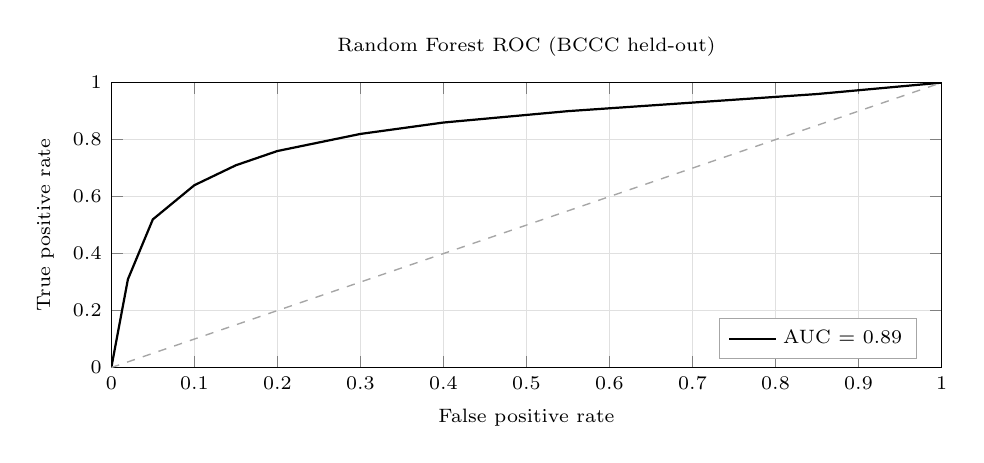
\begin{tikzpicture}
\begin{axis}[
 width=\linewidth,
 height=5.2cm,
 xlabel={False positive rate},
 ylabel={True positive rate},
 xmin=0, xmax=1,
 ymin=0, ymax=1,
 grid=both,
 grid style={black!12},
 tick label style={font=\scriptsize},
 label style={font=\scriptsize},
 title={\scriptsize Random Forest ROC (BCCC held-out)},
 title style={font=\scriptsize},
 legend style={font=\scriptsize, at={(0.97,0.03)}, anchor=south east, draw=black!35, fill=white},
]
\addplot[black, line width=0.8pt, mark=none]
 coordinates {
 (0,0) (0.02,0.31) (0.05,0.52) (0.10,0.64) (0.15,0.71)
 (0.20,0.76) (0.30,0.82) (0.40,0.86) (0.55,0.90) (0.70,0.93)
 (0.85,0.96) (1,1)
 };
\addlegendentry{AUC = 0.89}
\addplot[black!35, dashed, line width=0.5pt] coordinates {(0,0) (1,1)};
\end{axis}
\end{tikzpicture}

\vspace{4pt}
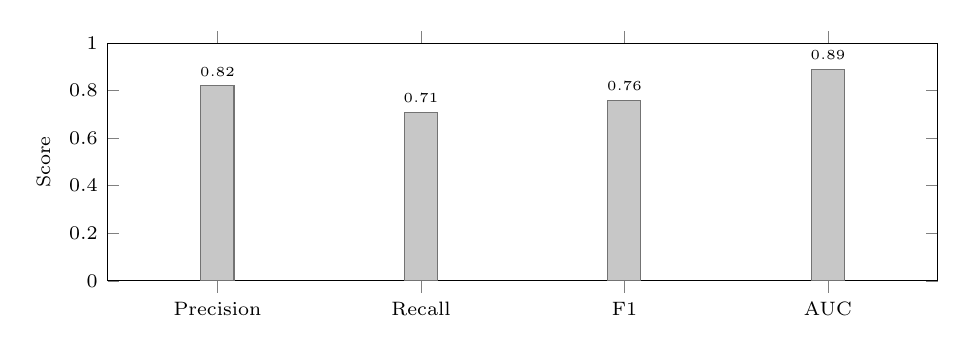
\begin{tikzpicture}
\begin{axis}[
 width=\linewidth,
 height=4.6cm,
 ybar,
 bar width=0.42cm,
 symbolic x coords={Precision, Recall, F1, AUC},
 xtick=data,
 ymin=0, ymax=1,
 ylabel={Score},
 tick label style={font=\scriptsize},
 label style={font=\scriptsize},
 nodes near coords={\pgfmathprintnumber[fixed, precision=2]{\pgfplotspointmeta}},
 every node near coord/.append style={font=\tiny},
 enlarge x limits=0.18,
]
\addplot[fill=black!22, draw=black!55] coordinates {
 (Precision, 0.82) (Recall, 0.71) (F1, 0.76) (AUC, 0.89)
};
\end{axis}
\end{tikzpicture}
\end{minipage}\hfill
\begin{minipage}[t]{0.48\linewidth}
\centering
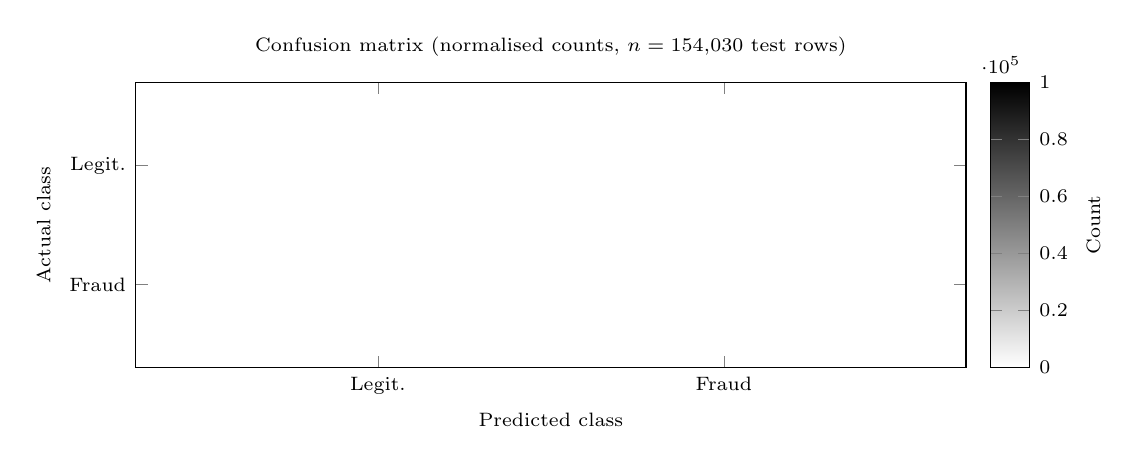
\begin{tikzpicture}
\begin{axis}[width=\linewidth, height=5.2cm, xlabel={Predicted class}, ylabel={Actual class}, xtick={0, 1}, ytick={0, 1}, xticklabels={Legit., Fraud}, yticklabels={Legit., Fraud}, tick label style={font=\scriptsize}, label style={font=\scriptsize}, title={\scriptsize Confusion matrix (normalised counts, $n=154{, }030$ test rows)}, title style={font=\scriptsize}, colorbar, colormap={greyscale}{color(0cm)=(white); color(1cm)=(black!)}, point meta min=0, point meta max=100000, colorbar style={font=\scriptsize, ylabel={Count}}, ]
\addplot[matrix plot, mesh/cols=2, mesh/rows=2, shader=flat corner, ] table[meta=z] {
 x y z
 0 0 98420
 1 0 1180
 0 1 820
 1 1 610
};
\end{axis}
\end{tikzpicture}

\vspace{4pt}
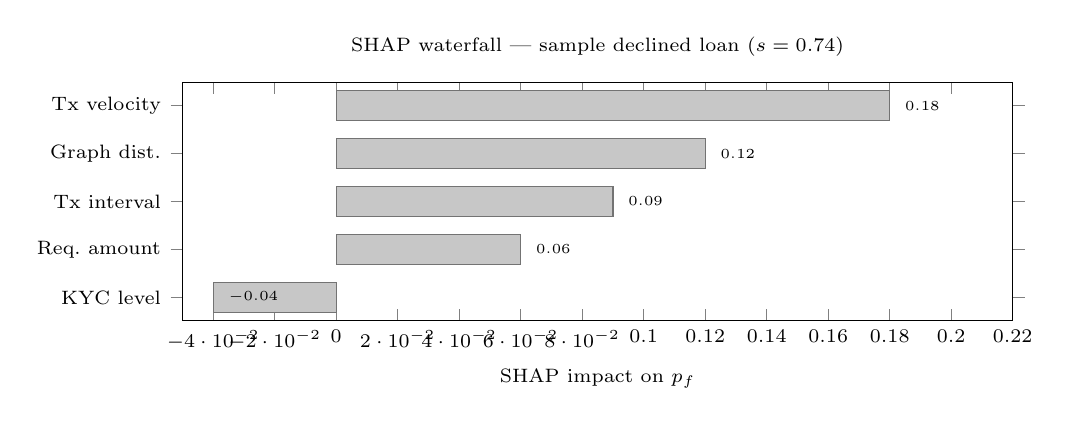
\begin{tikzpicture}
\begin{axis}[
 width=\linewidth,
 height=4.6cm,
 xbar,
 bar width=0.38cm,
 xmin=-0.05, xmax=0.22,
 symbolic y coords={%
 KYC level, Req.\ amount, Tx interval, Graph dist., Tx velocity%
 },
 ytick=data,
 xlabel={SHAP impact on $p_f$},
 tick label style={font=\scriptsize},
 label style={font=\scriptsize},
 title={\scriptsize SHAP waterfall --- sample declined loan ($s=0.74$)},
 title style={font=\scriptsize},
 nodes near coords={\pgfmathprintnumber[fixed, precision=2]{\pgfplotspointmeta}},
 every node near coord/.append style={font=\tiny, anchor=west, xshift=2pt},
 enlarge y limits=0.12,
]
\addplot[fill=black!22, draw=black!55] coordinates {
 (0.18,Tx velocity) (0.12,Graph dist.) (0.09,Tx interval)
 (0.06,Req.\ amount) (-0.04,KYC level)
};
\end{axis}
\end{tikzpicture}
\end{minipage}
\caption[Planned ML evaluation layout (post pre-thesis 2)]{Planned ML evaluation layout (post pre-thesis 2)}
\label{fig:ml-eval}
\end{figure}

\subsection{Explainability and Anomaly Detection Methodology}
\label{sec:ml-explainability}

Humans need to see \textit{why} a score was high, not just the number. This path is separate from the optional agent (Section~\ref{sec:optional-agent}).

Random Forest gives $p_f$ with \textbf{SHAP TreeExplainer} attributions per feature~[4]. Isolation Forest catches behaviour that looks nothing like normal clients---trained on non-fraud history only---and scores anomalies via path length (List of Formulas). Because IF scores are not probabilities, a stacking meta-learner maps $(p_f, s_{\text{IF}})$ to the single $s$ the contract reads.

IF has no native SHAP, so outliers get a \textbf{feature-deviation report}: top features vs.\ training median and percentile, e.g.\ \emph{``repayment interval variance at the 98th percentile; two hops from a flagged wallet.''}

\begin{figure}[H]
\centering
\BalancedDiagram{fig-ml-explainability.pdf}
\caption[Explainability and anomaly-detection flow]{Explainability and anomaly-detection flow}
\label{fig:ml-explainability}
\end{figure}

\begin{table}[H]
\centering
\begin{tabular}{p{2.2cm}p{3.2cm}p{7.8cm}}
\toprule
\tableheadcolor
\textbf{Audience} & \textbf{UI / channel} & \textbf{Content stored and displayed} \\
\midrule
Retail client & React loan status page & Top-3 SHAP reasons in plain language on decline; optional anomaly summary if score $\ge 0.7$ \\
Bank approver & Authority Brief dashboard & SHAP waterfall + anomaly deviation table + composite $s$; one-click approve / decline \\
Compliance auditor & \texttt{AI\_ML\_SECURITY\_LOG} & Full SHAP vector, IF score, feature JSON, model version hash, oracle tx hash \\
\bottomrule
\end{tabular}
\end{table}

The Authority Brief on the approver dashboard shows $s$, SHAP, and anomaly lines (example in Section~\ref{sec:optional-agent}). Every inference logs to \texttt{AI\_ML\_SECURITY\_LOG} with model version and oracle tx hash. ML advises; an approver still signs disbursement.

\section{Optional Conversational Agent Add-On (Phase III--IV)}
\label{sec:optional-agent}

Clients use the React dashboard by default. The conversational agent is an \textbf{optional add-on} (Phases~III--IV Could)---same API and contracts as the UI, never a gate on deposits or loans. Table~\ref{tab:mcp-tools} lists its tools; approver ML explainability (Section~\ref{sec:ml-explainability}) works without it.

The agent runs a six-step loop: (1)~message in via SSE; (2)~Qwen3-8B gets live account context in the system prompt; (3)~Q\&A answers from RAG, no tools; (4)~actions pick an MCP write tool and show a confirmation summary; (5)~user must say yes explicitly---no write without it; (6)~tool POSTs to Express.js, optional EIP-7702 signing, then status update to the client. Harness detail is in Appendix~\ref{app:agent-harness}.

\begin{table}[H]
\centering
\caption[MCP banking tools (17)]{MCP banking tools (17)}
\label{tab:mcp-tools}
\begin{tabular}{p{4.8cm}p{1.4cm}p{6.3cm}}
\toprule
\tableheadcolor
\textbf{Tool} & \textbf{Type} & \textbf{Maps to / Description} \\
\midrule
\texttt{get\_account\_state} & READ & SBT tier, loan count, savings balance \\
\texttt{get\_credit\_score} & READ & Current score, tier, next threshold \\
\texttt{get\_loan\_status} & READ & All active loans + next installment \\
\texttt{get\_installment\_schedule} & READ & Full repayment calendar \\
\texttt{get\_pool\_utilisation} & READ & Current Local Bank pool capacity \\
\texttt{get\_interest\_rate} & READ & Rate for client's credit tier \\
\texttt{get\_market\_data} & READ & ETH/USD, fiat/USD pairs, 30-day volatility \\
\texttt{get\_requirements} & READ & Documents + KYC needed for a given loan amount \\
\texttt{get\_session\_history} & READ & Search prior sessions (PostgreSQL full-text index) \\
\texttt{submit\_loan\_application} & WRITE$^{\dagger}$ & POST /api/loan/apply \\
\texttt{submit\_deposit} & WRITE$^{\dagger}$ & POST /api/savings/deposit \\
\texttt{submit\_fixed\_deposit} & WRITE$^{\dagger}$ & POST /api/savings/fixed-deposit \\
\texttt{pay\_installment} & WRITE$^{\dagger}$ & POST /api/installment/pay \\
\texttt{join\_group\_pool} & WRITE$^{\dagger}$ & POST /api/group/join \\
\texttt{submit\_kyc\_upgrade} & WRITE$^{\dagger}$ & POST /api/kyc/upgrade \\
\texttt{schedule\_payment\_reminder} & WRITE$^{\dagger}$ & POST /api/reminder/set \\
\texttt{submit\_group\_application} & WRITE$^{\dagger}$ & POST /api/group/apply \\
\bottomrule
\end{tabular}

\vspace{4pt}
\noindent\small$^{\dagger}$ Agent write tools require human confirmation before execution.
\end{table}

Every loan application gets an Authority Brief on the approver dashboard (UI or agent):

\begin{verbatim}
AUTHORITY BRIEF -- Loan Application #4821
-------------------------------------------------
Client tier: Silver (score: 512)
Requested amount: 150 USDC
Duration: 6 months
Collateral: 75 USDC (50% LTV)

ML Risk Score: 0.23 (LOW RISK)
SHAP breakdown:
 + On-time repayment rate: +0.41 (reduces risk)
 + Loan-to-income ratio: +0.18 (within safe range)
 - Wallet age: -0.09 (account < 6 months)
 - No prior completed loans: -0.27 (no repayment history)

ML system recommendation: APPROVE (decision support only)
Suggested interest: Base rate - 0.5% (Silver tier)

[ APPROVE ] [ REQUEST MORE INFO ] [DECLINE]
\end{verbatim}

\section{Graph Neural Network Extension}
\label{sec:gnn-extension}

Fraud often lives in \textit{who connects to whom}, not one transaction. As a stretch goal we would add GraphSAGE: wallets as nodes, transfers and tier links as edges, same 18 behaviour features as the Random Forest. The test is whether bank-hierarchy edges beat a flat graph on BCCC~[83]. Future Work only---if we have time, one before/after F1 or AUC table.

\section{Federated Learning Across Banking Tiers}
\label{sec:fl-fraud}

Local Banks would train on their own borrowers; the National Bank aggregates updates (FedAvg + differential privacy) and ships back a shared model---no raw data crosses borders. We turn federation on only after a bank hits \textbf{500 transactions}; until then everyone uses the public baseline. Future Work, not MVT.

\section{Formal Verification of Reserve Invariants (Certora)}
\label{sec:certora}

Beyond unit tests we plan two Certora proofs on reserve rules (Phase~IV MVT+):
\begin{itemize}[noitemsep]
\item Reserve never under-collateralised: \(\mathrm{totalReserve} \ge \mathrm{minReserveRatio} \cdot \mathrm{totalDeposited}\) on every path.
\item No over-allocation: the World Bank cannot allocate more to National Banks than it holds.
\end{itemize}
CVL sketches sit in Appendix~B; scope limits in Section~\ref{sec:research-limitations}.

\section{Foundry Invariant and Fuzz Test Suite}
\label{sec:foundry}

Hardhat covers integration and deployment; Foundry adds fuzzing and invariant checks. Together they catch different failure modes.

\paragraph{Three invariants under Foundry's stateful fuzzer.}
\begin{itemize}[noitemsep]
\item Solvency: outstanding loans never exceed total reserve.
\item Role segregation: one address cannot be both borrower and approver.
\item Capital flow: a single cross-tier move cannot break the minimum reserve ratio.
\end{itemize}

Each invariant is fuzzed for 10{,}000 runs in Phase~IV; any counterexample becomes a replay test in CI.

\section{On-Chain Economic Feasibility Simulation}
\label{sec:abm-sim}

Phase~IV runs a \textbf{reproducible stress test} on Polygon zkEVM Cardona: 300 synthetic clients, six banks, seed~42, 5\% mid-run defaults. A Foundry script walks the full lifecycle (apply $\to$ approve $\to$ disburse $\to$ repay) and writes a JSON manifest---tx hashes, reserve ratios, gas---for Appendix~C and Table~\ref{tab:gas-costs}. Results are reported as ranges; microfinance calibration stays in Future Work (Section~\ref{sec:future-work}).

\section{Real-Time Dashboard Pipeline and Runtime Monitoring}
\label{sec:realtime}

\begin{figure}[H]
\centering
\ActivityDiagram{fig-realtime-dashboard.pdf}
\caption[Real-time dashboard and runtime monitoring pipeline]{Real-time dashboard and runtime monitoring pipeline}
\label{fig:realtime-dashboard}
\end{figure}

Three pieces connect chain events to the UI (Figure~\ref{fig:realtime-dashboard}). A \textbf{The Graph subgraph} indexes contract events (\texttt{LoanRequested}, \texttt{Repayment}, \texttt{ReserveRatioUpdated}, and related emissions) so the React app can query history in milliseconds instead of polling RPC. A \textbf{WebSocket listener} pushes the same events to the browser via Socket.IO for live updates. \textbf{Tenderly} watches testnet contracts for large disbursements, repeat loan spam, reserve-ratio drops, failed calls, and governance pauses---and simulates txs before deployment demos.

\section{Transaction-State Machine for Frontend UX}
\label{sec:tx-state-machine}

\begin{figure}[H]
\centering
\BalancedDiagram{Ch4_loan-lifecycle-state-machine.pdf}
\caption[Transaction state machine of the loan lifecycle]{Transaction state machine of the loan lifecycle}
\label{fig:tx-state-machine}
\end{figure}

The frontend tracks every loan tx through five states (Figure~\ref{fig:tx-state-machine}): \texttt{idle} $\to$ \texttt{pending\_signature} $\to$ \texttt{submitted} $\to$ \texttt{confirming} $\to$ \texttt{success / error}. Each state has its own UI feedback. Wallet rejection (MetaMask 4001), contract revert, and network errors get separate messages so users know what failed and can retry.

\section{EIP-712 Authentication and API Hardening}
\label{sec:eip712-auth}

Users sign an EIP-712 message \texttt{(wallet, timestamp, nonce)} at login; the backend recovers the address and issues a 15-minute JWT (refresh tokens rotate on use). Each request carries a correlation ID from React through Express.js and FastAPI to the on-chain tx for end-to-end tracing. \texttt{slowapi} rate-limits by endpoint (5/min auth, 60/min reads, 10/min writes); logout blacklists the JWT in Redis. See Section~\ref{sec:defense-in-depth} for the full Layer~2 control set.

\noindent ML scores are decision support only---not auto-approval. Class imbalance, drift, and cold-start remain; GNN ablation, federated learning, and LLM red-teaming (Section~\ref{sec:llm-eval}) bound but do not remove them.

\section{Evaluation Methodology}
\label{sec:eval-method}

We tie each research question to something we can actually demonstrate on the prototype:
\begin{itemize}[noitemsep]
\item \textbf{RQ1:} Four-tier flows and roles vs.\ flat DeFi (Aave, Compound, MakerDAO).
\item \textbf{RQ2:} Testnet latency and gas; reserves and state changes visible on-chain.
\item \textbf{RQ3:} After pre-thesis~2, report precision, recall, F1, and AUC on BCCC~[83], plus SHAP explanations and audit logs. GNN ablation and testnet retrain are stretch goals.
\item \textbf{RQ4:} Full demo path (wallet $\to$ loan $\to$ approval $\to$ repayment) and Foundry invariant pass rate (Section~\ref{sec:foundry}). Deployment evidence lands in Phase~IV.
\item \textbf{RQ5:} Deposit and group-lending specs; Phase~IV simulation (Section~\ref{sec:abm-sim}) stress-tests reserves under default.
\end{itemize}

\subsection{LLM Assistant Evaluation Protocol}
\label{sec:llm-eval}

If the optional agent ships (Phase~IV Could), we run three checks: \textbf{Q\&A} on 200 policy prompts (exact numbers, similarity on prose); \textbf{tool use} on 50 scenarios (correct tool, params, confirmation summary---$\geq$95\%, always human-gated); and a \textbf{bypass red-team} of 20 adversarial prompts that must never trigger a write without explicit user consent.

\section{Implementation Phase Plan and Deliverables}

The build runs in four phases (I--IV), roughly three to four weeks each. Task registers below list effort by phase; Figures~\ref{fig:phase-roadmap}--\ref{fig:dev-toolchain} show the roadmap and toolchain.

\subsection{Phase I: Foundation and Infrastructure (Weeks 1--4)}

\textbf{Goal:} Contract skeleton, database migration, React shell with wallet connect.

\begin{table}[H]
\centering
\caption[Phase I task register]{Phase I task register}
\label{tab:phaseI-contracts}
\small
\begin{tabular}{p{1.8cm}p{1.8cm}p{7.5cm}p{1.5cm}}
\toprule
\tableheadcolor
\textbf{Task} & \textbf{Priority} & \textbf{Development Task} & \textbf{Effort (days)} \\
\midrule
DT-I.01 & Must & World Bank contract --- reserve management, national bank registration & 5 \\
DT-I.02 & Must & National Bank contract --- borrow from World Bank, lend to Local Banks & 5 \\
DT-I.03 & Must & Local Bank contract --- borrow from National Bank, lend to users & 5 \\
DT-I.04 & Must & Role-based access control --- WorldBankAdmin, NationalBankAdmin, LocalBankAdmin, BankUser, RetailClient & 3 \\
DT-I.05 & Should & Gas cost management --- initiator-pays pattern; Polygon low-fee design & 2 \\
DT-I.06 & Should & \texttt{InsuranceFund} contract --- 5\% interest capture, claims processing, default coverage disbursement & 4 \\
DT-I.07 & Should & \texttt{getReserveSummary} view function on each tier contract (PSR, reserve balance, insurance fund) & 2 \\
DT-I.08 & Should & Chainlink Price Feeds integration (fiat/USD pairs, ETH/USD via \texttt{AggregatorV3Interface}) & 3 \\
DT-I.09 & Should & Chainlink Proof of Reserve --- WorldBankReserve attestation & 2 \\
DT-I.10 & Should & Append-only \texttt{audit\_logs} PostgreSQL role + Row-Level Security policies & 2 \\
DT-I.11 & Should & Polygon zkEVM Cardona migration --- update RPC endpoints, chain IDs, factory addresses & 1 \\
DT-I.12 & Must & Full 20-entity database schema migration --- all tables including SESSIONS, AGENT\_ACTION\_LOG (with \texttt{injection\_scan\_flag}, \texttt{toolset\_name}), and all banking entities & 4 \\
DT-I.13 & Must & Core indexes and referential integrity constraints & 2 \\
DT-I.14 & Must & React frontend shell --- Vite build, routing, layout components & 3 \\
DT-I.15 & Must & WalletConnect integration --- wallet connection, address display, network switching & 2 \\
DT-I.16 & Should & Sessions and assets tables integration in frontend (dashboard stubs) & 2 \\
DT-I.17 & Should & Credit tier and interest rate schedule display & 2 \\
\multicolumn{3}{l}{\textit{Phase~I total estimated effort (Must-have):}} & \textit{29 days} \\
\multicolumn{3}{l}{\textit{Phase~I total estimated effort (all priorities):}} & \textit{48 days} \\
\bottomrule
\end{tabular}
\end{table}
\footnotetext{Must = MVT core; Should = important; Could = if time allows. Effort = person-days; streams run in parallel.}

\vspace{2pt}

\subsection{Phase II: Core Banking and On-Chain Lifecycle (Weeks 5--9)}

\textbf{Goal:} Full loan lifecycle on testnet---request, approval, installments, bank registration, SBT limits. Agent and multi-entity work defer to later phases.

\begin{table}[H]
\centering
\begin{tabular}{p{1.8cm}p{1.8cm}p{7.5cm}p{1.5cm}}
\toprule
\tableheadcolor
\textbf{Task} & \textbf{Priority} & \textbf{Development Task} & \textbf{Effort (days)} \\
\midrule
DT-II.01 & Must & Loan request submission with blockchain transaction & 5 \\
DT-II.02 & Must & Loan approval and rejection workflow with bank approver & 5 \\
DT-II.03 & Must & Installment payment system with automated schedule generation & 8 \\
DT-II.04 & Must & Borrowing limit enforcement (on-chain authoritative check per client SBT) & 5 \\
DT-II.05 & Should & Client--bank real-time chat system & 5 \\
DT-II.06 & Should & Income verification document upload and review & 5 \\
DT-II.07 & Must & Hierarchical bank registration (National $\to$ Local) & 5 \\
DT-II.08 & Should & Bank user management and approver designation & 3 \\
DT-II.09 & Should & Loan history and transaction tracking pages & 5 \\
DT-II.10 & Could & QR code generation for wallet addresses & 2 \\
DT-II.11 & Should & Responsive UI polish and error handling & 2 \\
DT-II.12 & Should & Authority Brief UI (SHAP breakdown for bank approver dashboard) & 5 \\
DT-II.13 & Should & Chainlink Automation for installment due-date checks and overdue flagging & 5 \\
DT-II.14 & Should & Credit tier schedule in Credit Passport SBT (Bronze $\to$ Diamond) & 3 \\
DT-II.15 & Should & \texttt{interest\_rate\_tier} table integration with Kinked Rate Model & 2 \\
DT-II.16 & Could & MCP tool server --- 17 banking tools wired to Express.js API (optional add-on) & 8 \\
DT-II.17 & Could & Agent chat interface (Qwen3-8B + tool calling + human-gate) & 8 \\
DT-II.18 & Could & EIP-7702 session key management (scope enforcement + TTL) & 5 \\
DT-II.19 & Could & \texttt{agent\_action\_log} table (append-only, FK to \texttt{sessions}) & 3 \\
\multicolumn{3}{l}{\textit{Phase~II total estimated effort (Must-have):}} & \textit{33 days} \\
\multicolumn{3}{l}{\textit{Phase~II total estimated effort (all priorities):}} & \textit{66 days} \\
\bottomrule
\end{tabular}
\end{table}

\vspace{2pt}

\subsection{Phase III: AI/ML Oracle Pipeline and Optional Agent (Weeks 10--13)}

\textbf{Goal:} Train models, deploy the scoring API, wire Chainlink Functions and the Authority Brief. Agent harness is Could-have.

\begin{table}[H]
\centering
\begin{tabular}{p{1.8cm}p{1.8cm}p{7.5cm}p{1.5cm}}
\toprule
\tableheadcolor
\textbf{Task} & \textbf{Priority} & \textbf{Development Task} & \textbf{Effort (days)} \\
\midrule
DT-III.01 & Must & Chainlink Functions oracle (primary ML score commitment): replaces commit-reveal relay; deploys \texttt{commitRiskScore} via Chainlink Functions DON & 6 \\
DT-III.02 & Must & Random Forest + Isolation Forest + SHAP pipeline wiring: FastAPI service computing 22 features, stacking meta-learner, calibrated composite score $s \in [1]$; client-facing SHAP plain-language explanation via Authority Brief UI & 7 \\
DT-III.03 & Should & Three-tier prompt constructor in Express.js (optional agent add-on) & 5 \\
DT-III.04 & Could & Session lineage + \texttt{get\_session\_history} MCP tool & 5 \\
DT-III.05 & Could & Context compression path + toolset scoping + Hook~2 & 9 \\
DT-III.06 & Could & Prompt injection scanning + confirmation audit hook (Hook~1) & 5 \\
DT-III.07 & Should & The Graph subgraph + WebSocket event listener for Reserve Transparency Dashboard & 4 \\
DT-III.08 & Should & SAR workflow: Isolation Forest $\to$ aml-alert $\to$ \texttt{freezeAccount}; compliance review queue integration & 4 \\
DT-III.09 & Should & Reserve Transparency Dashboard: live queries to The Graph subgraph & 3 \\
DT-III.10 & Could & GraphSAGE GNN ablation & 5 \\
DT-III.11 & Could & Federated learning aggregator & 7 \\
\multicolumn{3}{l}{\textit{Phase~III total estimated effort (Must-have):}} & \textit{13 days} \\
\multicolumn{3}{l}{\textit{Phase~III total estimated effort (all priorities):}} & \textit{55 days} \\
\bottomrule
\end{tabular}
\end{table}

\vspace{2pt}

\subsection{Phase IV: Verification, Evaluation, and Finalization (Weeks 14--16)}

\textbf{Goal:} On-chain simulation, Certora/Foundry checks, testnet evidence, optional LLM eval, final thesis revision.

\begin{table}[H]
\centering
\begin{tabular}{p{1.8cm}p{1.8cm}p{7.5cm}p{1.5cm}}
\toprule
\tableheadcolor
\textbf{Task} & \textbf{Priority} & \textbf{Development Task} & \textbf{Effort (days)} \\
\midrule
DT-IV.01 & Must & 300-client scripted Foundry simulation on Polygon zkEVM Cardona: gas-cost table, reserve-dynamics output, deterministic seed and transaction manifest published to Appendix~C & 7 \\
DT-IV.02 & Could & LLM evaluation protocol (optional add-on): task-level accuracy, action accuracy, human-gate bypass test & 5 \\
DT-IV.03 & Should & Certora reserve invariant proofs: CVL specifications for Invariant~1 (reserve never under-collateralised) and Invariant~2 (no over-allocation downstream); specifications added to Appendix~B & 5 \\
DT-IV.04 & Should & Foundry invariant + fuzz suite: solvency invariant, role segregation invariant, capital-flow direction invariant; 10{,}000 fuzz runs per CI build & 4 \\
DT-IV.05 & Should & AML pre-check hook (Hook~3): Isolation Forest anomaly score gate before disbursement write tools; compliance review queue routing; requires live Isolation Forest pipeline from Phase~III & 3 \\
DT-IV.06 & Could & Groth16 zkKYC circuit (Circom~2.0): government-ID possession proof without revealing PII; circuit design and input/output specification & 5 \\
DT-IV.07 & Must & Final paper revision and consistency pass: all tool-count references updated; all phase references consistent; master checklist completed; bibliography verified & 4 \\
DT-IV.08 & Must & Red-team testing and documentation: 20-payload injection red-team set; 20 bypass-attempt set; 10 session key scope enforcement scenarios; results documented in evaluation subsections & 3 \\
\multicolumn{3}{l}{\textit{Phase~IV total estimated effort (Must-have):}} & \textit{21 days} \\
\multicolumn{3}{l}{\textit{Phase~IV total estimated effort (all priorities):}} & \textit{38 days} \\
\bottomrule
\end{tabular}
\end{table}

\begin{table}[H]
\centering
\begin{tabular}{p{1.5cm}p{3.5cm}p{2cm}p{2cm}p{3cm}}
\toprule
\tableheadcolor
\textbf{Phase} & \textbf{Focus} & \textbf{Weeks} & \textbf{Tasks} & \textbf{Key deliverables} \\
\midrule
I & Foundation and infrastructure & 1--4 & DT-I.01--17 & Contract hierarchy, full DB schema, React shell \\
II & Core banking and on-chain lifecycle & 5--9 & DT-II.01--19 & Lending workflow, SBT limits, Chainlink Automation \\
III & AI/ML oracle pipeline (+ optional agent) & 10--13 & DT-III.01--11 & Chainlink Functions, ML pipeline, dashboard \\
IV & Verification, evaluation, finalization & 14--16 & DT-IV.01--08 & Certora, Foundry, simulation, testnet deploy \\
\bottomrule
\end{tabular}
\end{table}

\vspace{2pt}

\begin{figure}[H]
\centering
\ActivityDiagram{Ch4_four-phase-roadmap-sdlc.pdf}
\caption[Four-phase roadmap with SDLC mapping and progress]{Four-phase roadmap with SDLC mapping and progress}
\label{fig:phase-roadmap}
\end{figure}

\begin{figure}[H]
\centering
\HalfWidthDiagram{fig-phase-effort-bar.pdf}
\caption[Development effort by implementation phase]{Development effort by implementation phase}
\label{fig:phase-effort}
\end{figure}

\begin{figure}[H]
\centering
\ThesisIncludeGraphics[width=0.75\linewidth, height=0.54\textheight, keepaspectratio]{fig-optional-agent-addon.pdf}
\caption[Optional conversational agent add-on]{Optional conversational agent add-on}
\label{fig:optional-agent-addon}
\end{figure}

\begin{figure}[H]
\centering
\ActivityDiagram{Ch4_dev-verification-toolchain.pdf}
\caption[Planned development and verification toolchain]{Planned development and verification toolchain}
\label{fig:dev-toolchain}
\end{figure}

\section{SDLC Stage Mapping}

We map our four implementation phases to the seven stages of the Software Development Life Cycle (SDLC). Figure~\ref{fig:phase-roadmap} illustrates this mapping.

\begin{table}[H]
\centering
\caption[SDLC stage mapping]{SDLC stage mapping}
\label{tab:sdlc-mapping}
\begin{tabular}{p{0.5cm}p{2.5cm}p{4.5cm}p{5cm}}
\toprule
\tableheadcolor
\textbf{\#} & \textbf{SDLC Stage} & \textbf{Project Activity} & \textbf{Deliverable} \\
\midrule
1 & Planning & Feasibility studies; professor consultations; guideline review & Feasibility Report; Project Plan \\
2 & Requirements & System analysis; use case definitions; constraints identification & Use case diagrams; UC-1 through UC-5 \\
3 & Design & Three-layer architecture; DB schema (3NF); smart contract interfaces & Architecture diagrams; ERD; DFD \\
4 & Development & Phase I--IV: smart contracts, frontend, backend, AI/ML & Source code; DApp prototype \\
5 & Testing & Hardhat unit tests; Foundry fuzz; integration testing; AI/ML evaluation & Test reports; model metrics \\
6 & Deployment & Planned testnet deployment (Phase~IV); frontend (Vercel); backend (Render) & Testnet prototype manifest \\
7 & Maintenance & Monitoring; model retraining; bug fixes; iteration & Updated docs; retrained models \\
\bottomrule
\end{tabular}
\end{table}

\vspace{2pt}

\section{Design Decisions and Alternatives}
\label{sec:design-decisions}

For each major design decision, we evaluated alternatives and justified selections based on technical criteria, ecosystem maturity, and project constraints (Table~\ref{tab:design-decisions}; Figure~\ref{fig:design-decisions}).

\begin{table}[H]
\centering
\caption[Design decisions and alternatives considered]{Design decisions and alternatives considered}
\label{tab:design-decisions}
\begin{tabular}{p{3cm}p{3cm}p{3cm}p{4.5cm}}
\toprule
\tableheadcolor
\textbf{Decision Area} & \textbf{1st Choice} & \textbf{2nd Choice} & \textbf{Key Criterion} \\
\midrule
Methodology & Agile / Scrum & Incremental & Evolving scope, milestones \\
Architecture & DApp + Off-chain AI & Hybrid with Oracle & Gas cost, ML flexibility \\
Frontend & React + TypeScript & Vue + TypeScript & Web3 ecosystem maturity \\
Smart Contract & EVM (Solidity) & Solana (Rust) & Gas, control size, free testnets \\
Fraud Detection & Random Forest & XGBoost & SHAP compatibility, simplicity \\
Anomaly Detection & Isolation Forest & Autoencoder & Unsupervised; no labelled data needed \\
XAI Method & SHAP & LIME & Theoretical guarantees, regulatory fit \\
Database & PostgreSQL & SQLite & 3NF support, async queries \\
Hosting & Vercel + Render & Localhost only & \$0 cost, publicly accessible URL \\
Network (primary) & Polygon zkEVM Cardona & Polygon Amoy PoS & ZK validity proof security model vs.\ validator set assumption \\
Oracle mechanism & Chainlink Functions (DON) & Commit-reveal relay & Decentralised trust vs.\ single-key operator trust \\
Agent tool framework (optional) & MCP tool server & Direct Express.js API & Defined schema = safety boundary; Phase~III--IV Could \\
Agent session auth (optional) & EIP-7702 session keys & ERC-4337 paymasters & Key-level scope; optional add-on \\
Prompt construction (optional) & Three-tier assembly & Single ad-hoc string & Agent-only; Phase~III Could \\
Session memory (optional) & Lineage model & 10-turn window & Agent-only cross-session continuity \\
Tool exposure per turn (optional) & Named toolsets & Full 17-tool list & Agent attack-surface reduction \\
Write-tool enforcement (optional) & Confirmation audit hook & In-pipeline check & Agent write-path only \\
\bottomrule
\end{tabular}
\TableScreenshotEnd{Design Decisions: Evaluated Alternatives and Selection Rationale}
\end{table}

\vspace{2pt}

\begin{figure}[H]
\centering
\BalancedDiagram{Ch4_design-decisions-alternatives.pdf}
\caption[Key design decisions and alternatives considered]{Key design decisions and alternatives considered}
\label{fig:design-decisions}
\end{figure}

\subsection{Justification of Selected Technologies}

Selections follow Table~\ref{tab:design-decisions} in Section~\ref{sec:design-decisions}. One-line decision logic per row.

\textbf{1st choices:}
\begin{itemize}[noitemsep]
\item \textbf{Agile/Scrum} --- evolving scope; short sprints fit thesis window.
\item \textbf{DApp + off-chain AI} --- ML off-chain (cost); disbursement rules on-chain.
\item \textbf{React + TypeScript} --- strongest Wagmi/ethers wallet stack.
\item \textbf{EVM (Solidity)} --- OpenZeppelin, Slither/Mythril, free testnets.
\item \textbf{MUI} --- banking tables/forms without custom UI build.
\item \textbf{Random Forest} --- exact SHAP TreeExplainer; tabular + imbalanced labels~[4].
\item \textbf{Isolation Forest} --- unsupervised; scarce fraud labels.
\item \textbf{SHAP} --- stable attributions vs.\ LIME~[4].
\item \textbf{PostgreSQL} --- ACID; window queries for rolling limits; JSON columns.
\item \textbf{Vercel + Render} --- free public demo for examiners.
\item \textbf{Polygon zkEVM Cardona} --- ZK proofs for reserve claims; Amoy fallback.
\item \textbf{Chainlink Functions} --- DON consensus on score; OK latency for loan approval.
\item \textbf{MCP tool server} --- 17-tool schema caps agent; auditable.
\item \textbf{EIP-7702 session keys} --- tool list + cap + TTL in key; ERC-4337 for retail gas only.
\end{itemize}

\textbf{2nd choices (retained, not selected):}
\begin{itemize}[noitemsep]
\item \textbf{Waterfall} --- fixed scope; poor fit for research prototype.
\item \textbf{On-chain ML oracle} --- latency, cost, third-party dependency.
\item \textbf{Vue} --- thinner Web3 libraries.
\item \textbf{Solana} --- Rust curve; weaker audit toolchain in 8-week window.
\item \textbf{Tailwind} --- more UI time than MUI.
\item \textbf{XGBoost} --- approximate SHAP.
\item \textbf{Autoencoder} --- more data/tuning than IF here.
\item \textbf{LIME} --- unstable repeat explanations~[4].
\item \textbf{SQLite} --- no concurrent writes; weak window functions.
\item \textbf{Localhost only} --- no remote examiner demo.
\item \textbf{Amoy PoS} --- faster dev; weaker trust than ZK.
\item \textbf{Commit-reveal relay} --- Ph.~I--II fallback; trusts operator key.
\item \textbf{Direct Express API} --- no schema cap on agent.
\item \textbf{ERC-4337 for agent ops} --- scope in app layer, not key.
\end{itemize}

\section{Design Patterns}

Our system uses five design patterns:

\begin{itemize}[noitemsep]
\item \textbf{Singleton:} A singleton means that each primary contract is established a single time. Only one version is utilized by all ensuring a unified source of truth. Not everyone can create multiple versions of the contract.

\item \textbf{Observer:} Contracts generate alerts whenever actions occur such as loan requests. These alerts are processed by a service that updates the database. Notifications are not ignored; they receive attention.

\item \textbf{Adapter:} An Adapter is utilized by the wallet component to function with various wallet types (like MetaMask). Different wallets that adhere to the EIP-1193 standards can be easily integrated.

\item \textbf{Factory Pattern:} Each Local Bank creates individual loan and savings contract instances using a factory contract, ensuring all deployed instances follow the same security-audited interface and access control checks. The factory pattern prevents unauthorized contract deployment that could bypass the hierarchical governance structure.

\item \textbf{Proxy/Upgradeable Pattern:} Banking contracts must be upgradeable without losing stored state such as balances, credit scores, and loan histories. OpenZeppelin's transparent proxy pattern separates the contract's logic from its storage, allowing governance-approved upgrades to the logic layer while preserving all stored financial data. This pattern is essential for a long-lived banking system that must adapt to evolving regulatory requirements and security patches.

\item \textbf{Decorator Pattern (Prompt Assembly):} The three-tier prompt
constructor applies the Stable, Context, and Volatile tiers as successive
decorators on a base prompt object. Each tier adds its content without modifying
the structure established by prior tiers, enabling independent caching and testing
of each layer without rebuilding the full prompt.

\item \textbf{Chain of Responsibility (Lifecycle Hooks):} The write-tool middleware
stack implements a chain of responsibility: the confirmation audit hook, session
key scope pre-check, and AML pre-check each examine the request and either reject
it (HTTP~403) or pass it to the next hook. New policy controls are added as new
chain links without modifying existing route logic or the model
pipeline.

\item \textbf{Strategy Pattern (Toolset Selection):} The toolset selector
encapsulates the intent-classification algorithm as a replaceable strategy. The
current strategy is a lightweight keyword classifier; it can be replaced with a
fine-tuned intent model without changing the prompt constructor or the MCP tool
server, adhering to the Open/Closed Principle.
\end{itemize}

\section{Software Testing Strategy}

The testing strategy covers four layers of the system, each with defined acceptance criteria.

\begin{itemize}[noitemsep]
\item \textbf{Smart contract unit tests:} Numerous tests for smart contracts exist in our Hardhat environment. Over 12 tests are conducted to verify actions related to managing reserves, sign-ups, loans and access permissions. No scenarios such as depositing zero or executing disallowed actions are missed in these assessments. \textbf{Acceptance criterion:} all Hardhat unit tests pass with zero failures before any phase delivery.
\item \textbf{Integration testing:} Whole process checks are conducted for integration tests. Wallet connection, loan request, approval and repayment processes are evaluated on the network. No critical steps are excluded from the process. \textbf{Acceptance criterion:} end-to-end workflow completes successfully on testnet for representative scenarios (approval, rejection, repayment loop).
\item \textbf{AI/ML module verification:} Ensuring functionality is vital for our fraud and unusual activity detectors. Results are generated by the integration of the detectors with the overall system. \textbf{Acceptance criterion:} model inference endpoints return valid scores and explanations for test inputs without runtime errors.
\item \textbf{Frontend testing:} Website appearance is evaluated on Chrome, Firefox and mobile devices. Tests are conducted to ensure that functionality is maintained across various platforms. \textbf{Acceptance criterion:} core flows render and remain usable across desktop and mobile breakpoints without blocking UI defects.
\end{itemize}

%% CHAPTER 5: EVALUATION AND DISCUSSION
\chapter{Evaluation and Discussion}

\section{Performance Evaluation}
\label{sec:performance-eval}
\label{sec:cost-model}
\label{sec:gas-cost}

Pre-thesis~1 delivers specifications and planned checks, not live benchmarks. Component and economic feasibility are in Section~\ref{sec:feasibility}; RQ-level evaluation follows Section~\ref{sec:eval-method} after pre-thesis~2 (testnet deployment, gas measurement, ML metrics, MVT demo). On L2, projected gas per loan stays below interest earned; default stress is in Table~\ref{tab:default-scenarios}.

\section{Analysis of Design Solutions}
\label{sec:design-solutions-ch5}

Stack choices were scored on ecosystem maturity, zero-cost prototype constraints, and auditability (Table~\ref{tab:design-decisions}, Section~\ref{sec:design-decisions}). The selected path pairs EVM Solidity on zkEVM L2, PostgreSQL + FastAPI off-chain, and Chainlink Functions (with commit-reveal as an interim relay) for ML scores. The optional MCP agent and EIP-7702 session keys remain Phase~III--IV extensions outside the MVT.

\section{Final Design Adjustment}
\label{sec:final-design-adjustment}

The final pre-thesis design locks four adjustments before implementation: (i)~\textbf{stablecoin-first} retail lending (USDC/USDT, Section~\ref{sec:stablecoin-first}) to avoid ETH liability volatility; (ii)~\textbf{L2 deployment} for micro-loan gas economics; (iii)~\textbf{ML as decision support only}---human approvers and on-chain gates, no auto-disbursement; (iv)~\textbf{MVT scope} limited to the three-tier lending core, database schema, and dashboard---syndicated/tranched modules, full regulatory filing, and the conversational agent are deferred (Table~\ref{tab:mvt-checklist}).

\section{Feasibility Analysis}
\label{sec:feasibility}

\subsection{Technical Feasibility}

Each layer is specified against mature tooling; nothing requires bespoke infrastructure beyond standard testnets and open-source stacks (Table~\ref{tab:tech-feasibility}).

\begin{table}[H]
\centering
\caption[Technical feasibility assessment]{Technical feasibility assessment}
\label{tab:tech-feasibility}
\begin{tabular}{p{3cm}p{3cm}p{7.5cm}}
\toprule
\tableheadcolor
\textbf{Component} & \textbf{Assessment} & \textbf{Evidence} \\
\midrule
Smart contracts & Feasible (specified) & Solidity; Hardhat; OpenZeppelin; Phases~I--II \\
Frontend DApp & Feasible (specified) & React~18 + Wagmi/RainbowKit \\
Blockchain deployment & Feasible (planned) & Polygon zkEVM Cardona + Sepolia \\
AI/ML integration & Feasible with constraints & RF + IF + SHAP; Chainlink Functions Phase~III \\
Optional agent & Feasible (deferred) & MCP + Qwen3-8B; Phase~III--IV; outside MVT \\
Database backend & Feasible & PostgreSQL 20-entity schema (3NF); FastAPI \\
\bottomrule
\end{tabular}
\end{table}

\vspace{2pt}

\subsection{Economic Feasibility}

The academic prototype can run at \textbf{zero direct cost}; scaled hosting is a separate pilot concern (Table~\ref{tab:economic-feasibility}). L2 gas keeps small loans viable versus mainnet; spread revenue and default scenarios are modelled in Section~\ref{sec:statistical-analysis}.

\begin{table}[H]
\centering
\caption[Economic feasibility --- zero-cost prototype]{Economic feasibility --- zero-cost prototype}
\label{tab:economic-feasibility}
\begin{tabular}{p{4cm}p{2.5cm}p{7cm}}
\toprule
\tableheadcolor
\textbf{Cost Category} & \textbf{Estimate} & \textbf{Notes} \\
\midrule
Blockchain deployment & \$0 & Public testnets \\
Frontend / backend hosting & \$0 & Vercel / Render free tiers or localhost \\
AI/ML training & \$0 & Local machine or Colab free tier \\
Development tools & \$0 & Hardhat, VS Code, Git (open-source) \\
\textbf{Total prototype} & \textbf{\$0} & Pilot ops $\approx$\$500--\$2{,}000/month at scale \\
\bottomrule
\end{tabular}
\end{table}

\vspace{2pt}

\subsection{Risk Feasibility}

Main delivery risks and mitigations are summarised in Table~\ref{tab:risk-taxonomy}; smart-contract and regulatory items dominate severity.

\begin{table}[H]
\centering
\caption[Risk taxonomy and mitigation]{Risk taxonomy and mitigation}
\label{tab:risk-taxonomy}
\begin{tabular}{p{3cm}p{4cm}p{1.5cm}p{5cm}}
\toprule
\tableheadcolor
\textbf{Risk Category} & \textbf{Description} & \textbf{Severity} & \textbf{Mitigation} \\
\midrule
Partner non-cooperation & Key partners decline to join & Medium & Testnet pilots; open-source replication \\
Smart contract vulnerability & Logic exploit & High & OpenZeppelin; audits; pause mechanism \\
Regulatory adversity & Jurisdiction blocks retail crypto & Medium & Testnet-only prototype; sandbox path \\
AI/ML model degradation & Fraud model drift & Low & Retraining; human-in-the-loop; SHAP review \\
\bottomrule
\end{tabular}
\end{table}

\vspace{2pt}

\subsection{Regulatory Feasibility}
\label{sec:mica-compliance}

Retail stablecoin lending must align with MiCA, GENIUS Act, and EU AI Act expectations; CWB uses authorised stablecoins and keeps PII off-chain (Table~\ref{tab:mica-mapping}). Full conformity files and national licensing remain future work; pre-thesis scope is testnet demonstration only.

\begin{table}[H]
\centering
\caption[Regulatory design controls (selected)]{Regulatory design controls (selected)}
\label{tab:mica-mapping}
\begin{tabular}{p{3.2cm}p{4.6cm}p{5.8cm}}
\toprule
\tableheadcolor
\textbf{Statute / Article} & \textbf{Requirement} & \textbf{CWB Control} \\
\midrule
MiCA Art.~16 & Authorised EMT issuer & Uses USDC/USDT; does not issue \\
MiCA Art.~36 & 1{:}1 reserve backing & Issuer attestations before pool acceptance \\
EU AI Act (credit scoring) & High-risk AI from Aug.~2026~ & Human approver gate; SHAP + audit log \\
GDPR Art.~17 & Right to erasure & PII off-chain only; hashes on-chain \\
\bottomrule
\end{tabular}
\end{table}

\section{Statistical Analysis}
\label{sec:statistical-analysis}
\label{sec:interest-rates}

The tables below model spread revenue, ETH-price sensitivity, and default stress at full-deployment scale (planning assumptions only; not observed platform data). Interest tiers follow the 3\%/5\%/8\% hierarchy (Figure~\ref{fig:apr-spread}).

\begin{table}[H]
\centering
\caption[Revenue projection assumptions]{Revenue projection assumptions}
\label{tab:revenue-assumptions}
\begin{tabular}{p{6cm}p{7.5cm}}
\toprule
\tableheadcolor
\textbf{Parameter} & \textbf{Value} \\
\midrule
Reference ETH price & \$2{,}500 (planning mid-point, Feb 2026) \\
World Bank $\to$ National Bank & 3\% APR \\
National Bank $\to$ Local Bank & 5\% APR \\
Local Bank $\to$ Client & 8\% APR \\
Average loan term & 12 months \\
Default rate provision (base) & 8\% \\
Origination fee & 0.25\% per disbursement \\
\bottomrule
\end{tabular}
\end{table}

\vspace{2pt}

\begin{table}[H]
\centering
\caption[ETH-price sensitivity of spread revenue]{ETH-price sensitivity of spread revenue}
\begin{tabular}{@{}lccc@{}}
\toprule
\tableheadcolor
\tableheadfont ETH Price & \tableheadfont Loan Base & \tableheadfont Spread Revenue & \tableheadfont Incl.\ Fees (est.) \\
\midrule
\$2{,}000 & \$1.376B & \$110.1M & \$120--128M \\
\rowcolor{RowShade}
\$2{,}500 (base) & \$1.720B & \$137.6M & \$150--159M \\
\$3{,}000 & \$2.064B & \$165.1M & \$180--191M \\
\bottomrule
\end{tabular}
\end{table}

\vspace{2pt}

\begin{table}[H]
\centering
\caption[Default-rate sensitivity]{Default-rate sensitivity}
\label{tab:default-scenarios}
\begin{tabular}{@{}lccp{4.8cm}@{}}
\toprule
\tableheadcolor
\tableheadfont Scenario & \tableheadfont Default rate & \tableheadfont Annual loss & \tableheadfont Basis \\
\midrule
Optimistic & 3.7\% & \$7.4M & Mature MFI benchmarks~ \\
\rowcolor{RowShade}
Base case & 8\% & \$16M & New platform, limited history \\
Stress & 15\% & \$30M & Thin credit history, volatile collateral \\
\bottomrule
\end{tabular}
\end{table}

\begin{figure}[H]
\centering
\HalfWidthDiagram{fig-revenue-by-tier.pdf}
\caption[Annual revenue projection (10-year maturity)]{Annual revenue projection (10-year maturity)}
\label{fig:revenue-by-tier}
\end{figure}

\begin{figure}[H]
\centering
\HalfWidthDiagram{fig-apr-spread.pdf}
\caption[Hierarchical interest-rate spread (APR)]{Hierarchical interest-rate spread (APR)}
\label{fig:apr-spread}
\end{figure}

\section{Comparisons and Relationships}
\label{sec:comparisons-relationships}

\begin{table}[H]
\centering
\caption[Market segments with supporting data]{Market segments with supporting data}
\label{tab:market-sizing-ch5}
\begin{tabular}{p{3.5cm}p{6.5cm}p{3cm}}
\toprule
\tableheadcolor
\textbf{Segment} & \textbf{Description} & \textbf{Estimated Scale} \\
\midrule
TAM & Global DeFi lending; remittances; MSME gap~[8, 15, 20] & \$55B -- 5T+ \\
SAM & Institutional hierarchical lending; emerging-market credit & \$5B -- 15B \\
SOM & Testnet pilots; sandbox partnerships & \$50 -- 200M \\
\bottomrule
\end{tabular}
\end{table}

\vspace{2pt}

\begin{table}[H]
\centering
\caption[Target customer segment profile]{Target customer segment profile}
\label{tab:customer-segment-ch5}
\begin{tabular}{p{3.5cm}p{10cm}}
\toprule
\tableheadcolor
\textbf{Characteristic} & \textbf{Description} \\
\midrule
Primary users & Tier~1--3 bank operators; Tier~4 retail via Local Banks \\
Loan range & Micro/SME at Local Bank tier; larger exposures via syndication \\
Key pain points & Opaque reserves; flat DeFi pools; weak explainability in on-chain lending \\
\bottomrule
\end{tabular}
\end{table}

\vspace{2pt}

\begin{table}[H]
\centering
\caption[Partner categories and roles]{Partner categories and roles}
\label{tab:partner-categories-ch5}
\begin{tabular}{p{3.5cm}p{4.5cm}p{5.5cm}}
\toprule
\tableheadcolor
\textbf{Partner Category} & \textbf{Role} & \textbf{Incentive} \\
\midrule
Financial regulators & Sandbox oversight & On-chain audit trails \\
Banking institutions & National/Local Bank nodes & Reserve access; lower settlement friction \\
Oracle providers & Chainlink DON, indexing & Unified oracle stack \\
Academic partners & ML / formal-verification review & Datasets; co-publication \\
\bottomrule
\end{tabular}
\end{table}

\vspace{2pt}

No current protocol combines four-tier hierarchy, explainable ML governance, and programmable group lending. Table~\ref{tab:competitor-detailed} contrasts representative projects on the dimensions that matter for CWB.

\begin{table}[H]
\centering
\caption[Competitive feature comparison]{Competitive feature comparison}
\label{tab:competitor-detailed}
\begin{tabular}{p{4cm}p{5cm}p{4.5cm}}
\toprule
\tableheadcolor
\textbf{Feature} & \textbf{Typical competitors} & \textbf{Crypto World Bank} \\
\midrule
Hierarchical lending tiers & Flat pools (Aave, Compound) & Four-tier World $\to$ Client flow \\
Governance-controlled rates & Algorithmic pool rates only & Tier-bounded contract parameters \\
AI-assisted risk scoring & Rare in DeFi lending & RF + SHAP + anomaly path to oracle \\
Retail + institutional access & Often one or the other & Retail via Local Bank; banks at upper tiers \\
\bottomrule
\end{tabular}
\end{table}

\section{Discussion}
\label{sec:ch5-discussion}
\label{sec:research-limitations}
\label{sec:bangladesh-reg}

This pre-thesis specifies architecture and planned evaluation; deployment evidence, trained models, and formal proofs arrive after pre-thesis~2. Five examiner-facing limits are recorded explicitly:

\begin{itemize}[noitemsep]
\item \textbf{Novelty is compound, not absolute}---Maple, Goldfinch, and Morpho cover parts of institutional credit; the claim is the four-tier reserve stack plus explainable oracle ML plus group liability in one open design.
\item \textbf{BCCC is a baseline only}---flat-pool fraud labels may not transfer to hierarchical CWB flows without testnet retraining.
\item \textbf{Testnet scope}---workshop-grade evidence needs benchmarks and reproducible repos; MVT deployment supplies the empirical layer.
\item \textbf{Group lending}---on-chain cosigning is not social solidarity; BRAC/Grameen statistics inform design only.
\item \textbf{Oracle and economics}---scores attach at origination; collusion and model drift remain open; Certora proofs state assumptions explicitly.
\end{itemize}

The prototype runs on public testnets with test tokens only. Jurisdiction-specific pilots (e.g.\ regulatory sandboxes) are future work; the architecture is global L2 institutional DeFi, not a single-country rollout claim.


%% CHAPTER 6: CONCLUSION
\chapter{Conclusion}

The Crypto World Bank addresses a \textbf{multi-party coordination and trust} problem at the heart of hierarchical development finance. Existing DeFi lending protocols collectively manage over \$55~billion in TVL~[8], yet they rely on flat, single-tier pool designs that cannot model how capital actually moves between multilateral institutions, national banks, local lenders, and clients. This work proposes a four-tier institutional hierarchy with cross-tier, same-tier, and upward lending flows, governed by transparent rules for network membership, business operations, and technology infrastructure.

The platform is grounded in the six core functions of a bank---deposit mobilization, credit allocation, payment and settlement, risk intermediation, liquidity management, and ancillary services---but encodes them as publicly verifiable on-chain rules rather than discretionary enforcement by a trusted central authority. Reserve ratios, interest adjustments, group consent, and the full loan book are enforced and auditable in real time. A further distinctive capability is \textbf{multi-entity co-lending and co-funding}: at the retail level, solidarity groups can pool collateral and borrow together under mutual liability, drawing on the structural logic of Grameen Bank and BRAC; at the institutional level, multiple banks can co-fund a single loan or share risk across senior and junior tranches---mechanisms that no existing DeFi protocol combines in one open architecture.

This thesis contributes four scoped advances---hierarchical lending architecture, programmable group lending, explainable AI-assisted credit governance, and privacy-preserving compliance identity---as detailed in Section~\ref{sec:research-contribution}:
\begin{itemize}[noitemsep]
\item A four-tier DeFi architecture that mirrors multilateral development-finance capital flows, with reserve enforcement at every tier (Section~\ref{sec:research-limitations})
\item Programmable joint-liability group lending with over-indebtedness controls (Section~\ref{sec:over-indebt})
\item Oracle-mediated fraud and credit scoring with explainable outputs for approvers and clients (Sections~\ref{sec:ml-explainability},~\ref{sec:ml-workload})
\item A privacy-preserving identity and compliance pathway combining zero-knowledge proofs with decentralized identifiers (Section~\ref{sec:identity})
\end{itemize}
These contributions are positioned against the institutional-DeFi landscape in Section~\ref{sec:lit-institutional} and against the MiCA / GENIUS Act / EU AI Act frontier in Section~\ref{sec:mica-compliance}.

Analysis of 20+ competing projects in DeFi lending, institutional credit, banking infrastructure, and financial inclusion confirms that no current system combines multi-level lending, interbank mechanisms, and graded borrower access in one decentralized architecture. Institutional adoption---from the World Bank FundsChain initiative~[35] to JPMorgan Kinexys~ and R3 Corda's \$17~billion in tokenized assets~---shows that blockchain-based financial infrastructure is both technically feasible and institutionally demanded. The Crypto World Bank extends this trajectory from settlement and fund tracking into an open, hierarchically governed lending system at the intersection of institutional finance, decentralized lending, and financial inclusion---a combination still largely unaddressed in both academic literature and commercial practice.

At the pre-thesis stage, this report delivers a fully specified architecture, market and partnership framing, and phased implementation roadmap. The hierarchical lending workflow, tiered governance, capital-flow design, and planned explainable analytics layer are specified in depth; deposit products, group lending, multi-entity cross-tier operations, retail payment rails, formal verification, and runtime monitoring remain at the design level for final-thesis implementation per the Minimum Viable Thesis checklist (Section~\ref{sec:mvt-checklist}).

\section{Future Work}
\label{sec:future-work}

The remaining work falls into three directions: completing the final-thesis deliverable, extending into everyday banking, and pursuing longer-term research.

\paragraph{Final thesis priorities.}
\begin{itemize}[noitemsep]
\item \textbf{Complete hierarchical lending.} End-to-end cross-tier fund transfers, interest accrual, installment scheduling, and cascading repayment across all four tiers (Appendix~B).
\item \textbf{Stablecoin-first deployment.} USDC at retail tiers with MiCA / GENIUS Act mapping validated against deployed configuration (Sections~\ref{sec:stablecoin-first},~\ref{sec:mica-compliance}).
\item \textbf{Deposit and credit products.} Savings, fixed deposits, group lending with over-indebtedness controls, and liquidation handling (Sections~\ref{sec:savings-vault},~\ref{sec:over-indebt},~\ref{sec:liquidation}).
\item \textbf{Explainable analytics integration.} Connect fraud and credit scoring into live loan approvals via the oracle pipeline (Sections~\ref{sec:ml-explainability},~\ref{sec:ml-workload}).
\item \textbf{Simulation, verification, and monitoring.} Testnet simulation, reserve invariant proofs, and live transparency dashboards (Sections~\ref{sec:abm-sim},~\ref{sec:certora},~\ref{sec:realtime}).
\end{itemize}

\paragraph{Retail and everyday banking (post-MVT).}
\label{sec:future-retail-payments}

Before the platform can support everyday spending with stablecoins---not only lending and installment servicing---it must close gaps in remittance, merchant acceptance, and cash-like deposit/withdrawal identified in Section~\ref{sec:scopes-challenges} and grounded in the literature synthesis of Section~\ref{sec:lit-retail-payments}:
\begin{itemize}[noitemsep]
\item \textbf{Client-to-client remittance.} KYC-gated, compliance-checked transfers between registered clients under Local Bank sponsorship (Section~\ref{sec:tiered-kyc}).
\item \textbf{Fiat on/off-ramp integration.} Licensed payment-service APIs so clients can fund balances and withdraw to local currency---the binding constraint identified by Du et al.~[110] and CPMI.
\item \textbf{Merchant checkout.} Invoice-based payment requests and settlement for registered merchants, evaluated against the CLEAR framework of Li et al..
\item \textbf{Consumer protection.} Deposit insurance, dispute resolution, and retail FX conversion before off-ramp or cross-border remittance (Section~\ref{sec:banking-products}).
\end{itemize}
No prior work composes these retail rails with hierarchical development-finance lending in one architecture (Section~\ref{sec:lit-retail-payments}).

\paragraph{Longer-term research.}
\begin{itemize}[noitemsep]
\item \textbf{Graph-based fraud detection.} Hierarchical lending graph ablation on BCCC~[83] (Section~\ref{sec:gnn-extension}).
\item \textbf{Federated learning across banks.} Privacy-preserving fraud detection benchmarked against FedFraud~ (Section~\ref{sec:fl-fraud}).
\item \textbf{Privacy-preserving compliance.} Zero-knowledge AML and KYC circuits with FATF Travel Rule support (Section~\ref{sec:upward-flow}).
\item \textbf{Formal verification and domain adaptation.} Multi-tier reserve proofs~ and ML model transfer from flat-pool to hierarchical transaction data.
\item \textbf{Regulatory and retail evaluation.} EU AI Act conformity for credit scoring~ and CLEAR-framework assessment of retail payment modules.
\end{itemize}

\appendix

\chapter{Database Schema Reference}
\label{app:db-schema-reference}

Physical-schema detail for Chapter~3. B-tree indexes support rolling borrowing-limit windows, overdue installments, and agent audit queries (Table~\ref{tab:indexing-strategy}). Core functional dependencies are in Table~\ref{tab:functional-deps}; on-chain rules remain authoritative for limits and loan state.

\section{Indexing Strategy}

\begin{table}[H]
\centering
\caption[Indexing strategy]{Indexing strategy}
\label{tab:indexing-strategy}
\begingroup
\footnotesize
\setlength{\tabcolsep}{4pt}
\renewcommand{\arraystretch}{1.2}
\begin{tabular}{@{}%
 >{\raggedright\arraybackslash}p{0.19\linewidth}%
 >{\raggedright\arraybackslash}p{0.41\linewidth}%
 >{\raggedright\arraybackslash}p{0.36\linewidth}@{}}
\toprule
\tableheadcolor
\textbf{Index} & \textbf{Table / Column(s)} & \textbf{Rationale} \\
\midrule
\texttt{idx\_loan\_borrower} &
 \texttt{LOAN\_REQUEST}(\texttt{borrower\_id}) &
 Borrower loan history. \\
\texttt{idx\_loan\_status} &
 \texttt{LOAN\_REQUEST}(\texttt{status}) &
 Active vs.\ closed loans. \\
\texttt{idx\_installment\_due} &
 \texttt{INSTALLMENT}(\texttt{due\_date}, \texttt{status})\newline
 \texttt{WHERE status = 'PENDING'} &
 Overdue installment detection. \\
\texttt{idx\_txn\_created} &
 \texttt{TRANSACTION}(\texttt{created\_at}) &
 Rolling borrowing-limit windows. \\
\texttt{idx\_txn\_borrower} &
 \texttt{TRANSACTION}(\texttt{borrower\_id}) &
 Per-borrower history. \\
\texttt{idx\_market\_symbol} &
 \texttt{MARKET\_DATA}(\texttt{symbol},\newline
 \texttt{recorded\_at}) &
 Price feed time series. \\
\texttt{idx\_loan\_bank\_status} &
 \texttt{LOAN}(\texttt{local\_bank\_id}, \texttt{status},\newline
 \texttt{created\_at DESC}) &
 Bank loan queues. \\
\texttt{idx\_loan\_client\_active} &
 \texttt{LOAN}(\texttt{client\_id}, \texttt{status})\newline
 \texttt{WHERE status = 'ACTIVE'} &
 Open-loan count per client. \\
\texttt{idx\_agent\_client\_date} &
 \texttt{AGENT\_ACTION\_LOG}(\texttt{client\_id},\newline
 \texttt{created\_at DESC}) &
 Agent action history. \\
\texttt{idx\_agent\_status} &
 \texttt{AGENT\_ACTION\_LOG}(\texttt{status})\newline
 \texttt{WHERE status = 'PENDING'} &
 Pending agent actions. \\
\texttt{idx\_aiml\_score} &
 \texttt{AI\_ML\_LOG}(\texttt{anomaly\_score DESC})\newline
 \texttt{WHERE anomaly\_score > 0.5} &
 AML alert queue. \\
\texttt{idx\_session\_parent} &
 \texttt{SESSIONS}(\texttt{parent\_session\_id})\newline
 \texttt{WHERE parent\_session\_id IS NOT NULL} &
 Session lineage. \\
\bottomrule
\end{tabular}
\endgroup
\end{table}

\section{Functional Dependencies}

\begin{table}[H]
\centering
\caption[Representative functional dependencies]{Representative functional dependencies}
\label{tab:functional-deps}
\footnotesize
\begin{tabular}{p{3cm}p{5.5cm}p{5cm}}
\toprule
\tableheadcolor
\textbf{Relation} & \textbf{Functional Dependency} & \textbf{Notes} \\
\midrule
LOAN\_REQUEST & \texttt{request\_id} $\to$ all attributes & Application primary key. \\
LOAN & \texttt{loan\_request\_id} $\to$ \texttt{loan\_id} & 1:1 request to disbursement. \\
BORROWING\_LIMIT & \texttt{borrower\_id} $\to$ limits, timestamps & 1:1; enforced on-chain. \\
BORROWER & \texttt{wallet\_address} $\to$ \texttt{borrower\_id}, \ldots & Unique wallet in prototype. \\
INSTALLMENT & \texttt{loan\_id, installment\_number} $\to$ amount, due, status & Composite key. \\
SESSIONS & \texttt{session\_id} $\to$ client, scope, expiry & MCP session + EIP-7702 scope. \\
AGENT\_ACTION\_LOG & \texttt{action\_id} $\to$ session, tool, status, tx hash & Write-tool audit trail. \\
INTEREST\_RATE\_TIER & \texttt{tier\_id} $\to$ rates, kink params & Normalised rate schedule. \\
\bottomrule
\end{tabular}
\end{table}

\chapter{Optional Agent Harness Reference}
\label{app:agent-harness}

Optional Phase~III--IV add-on only (Section~\ref{sec:optional-agent}). One shared Qwen3-8B model; personalisation comes from per-user context injected each turn:

\begin{verbatim}
{
 "client_id": "0xABC...", "credit_tier": "Silver",
 "active_loans": [{"loan_id": "L-4821", "next_due": "2026-06-15"}],
 "conversation_history": ["...last 10 turns..."]
}
\end{verbatim}

Prompt assembly uses three tiers: \textbf{stable} (persona + tool schema), \textbf{context} (rates, KYC matrix), and \textbf{volatile} (live on-chain state + recent turns). Child sessions store a compression summary when the context window fills. Write tools require logged user confirmation; middleware checks session-key scope and AML flags before POST.

\begin{table}[H]
\centering
\caption[Agent toolsets]{Agent toolsets}
\begin{tabular}{p{3.5cm}p{9cm}}
\toprule
\tableheadcolor
\textbf{Toolset} & \textbf{Tools visible} \\
\midrule
\texttt{read\_only} & Nine read tools (default). \\
\texttt{loan\_actions} & Reads + loan / installment / group writes. \\
\texttt{account\_management} & Reads + deposit, KYC, reminder writes. \\
\bottomrule
\end{tabular}
\end{table}

\chapter{Technology Stack}

The optional in-product assistant uses a local Qwen3-8B endpoint behind the same Express.js API as the React UI. Figures~\ref{fig:local-llm-mermaid} and~\ref{fig:local-llm-tikz} show the request path; Table~\ref{tab:tech-stack} lists the full stack.

\begin{figure}[H]
\centering
\OnePageDiagram{fig-local-llm-compact.pdf}
\caption[Optional AI banking agent request path (add-on)]{Optional AI banking agent request path (add-on)}
\label{fig:local-llm-mermaid}
\end{figure}

\begin{figure}[H]
\centering
\OnePageDiagram{fig-local-llm.pdf}
\caption[Optional AI agent data flow]{Optional AI agent data flow}
\label{fig:local-llm-tikz}
\end{figure}

\begin{table}[H]
\centering
\caption[Technology stack summary]{Technology stack summary}
\label{tab:tech-stack}
\footnotesize
\begin{tabular}{p{3cm}p{4cm}p{6.5cm}}
\toprule
\tableheadcolor
\textbf{Layer} & \textbf{Technology} & \textbf{Notes} \\
\midrule
Smart Contract & Solidity 0.8.20, OpenZeppelin & ReentrancyGuard, AccessControl \\
Frontend & React 18, TypeScript, MUI & Wagmi / RainbowKit / Viem \\
Backend & Express.js, PostgreSQL, FastAPI & REST + ML scoring service \\
Network & Polygon zkEVM Cardona & Sepolia fallback \\
AI (optional) & Qwen3-8B, MCP (17 tools) & Human confirmation on writes \\
Oracles & Chainlink Functions, Feeds, PoR, Automation & ML scores + rates + upkeep \\
Indexing & The Graph subgraph & Dashboard / audit queries \\
\bottomrule
\end{tabular}
\end{table}

\chapter{Smart Contract Capabilities}

Fifteen modular contracts: three core (Phase~I), six banking products (Phase~II), six multi-entity modules (Phases~II--III). Appendix~D shows the Tier~1 public interface.

\begin{table}[H]
\centering
\caption[Contract inventory by phase]{Contract inventory by phase}
\label{tab:contract-inventory}
\footnotesize
\begin{tabular}{p{2.2cm}p{4.2cm}p{7.8cm}}
\toprule
\tableheadcolor
\textbf{Phase} & \textbf{Contract} & \textbf{Role} \\
\midrule
I & WorldBankReserve, NationalBank, LocalBank & Reserve, allocation, loan lifecycle, \texttt{freezeAccount} \\
II & SavingsVault, FixedDeposit, GroupLendingPool, FXModule, InsuranceFund, CurrentAccount & Deposits, groups, FX, insurance, transactions \\
II--III & InterBankLendingPool, UpwardDepositFacility, SyndicatedLoan & Same-tier liquidity, upward flow, syndication \\
III & TranchedPool, TreasurySwap, NettingEngine & Tranching, treasury FX, multilateral netting \\
\bottomrule
\end{tabular}
\end{table}

\chapter*{Appendix C: Planned Testnet Deployment Manifest}
\phantomsection
\addcontentsline{toc}{chapter}{Appendix C: Planned Testnet Deployment Manifest}

Planned Polygon zkEVM Cardona manifest (Phase~IV). Addresses are filled after deployment under \texttt{deployments/cardona/}; nothing is live at pre-thesis submission.

\begin{table}[H]
\centering
\caption[Planned Cardona testnet deployment manifest]{Planned Cardona testnet deployment manifest}
\label{tab:cardona-manifest}
\footnotesize
\begin{tabular}{@{}%
 >{\raggedright\arraybackslash}p{0.22\linewidth}%
 >{\raggedright\arraybackslash}p{0.26\linewidth}%
 >{\raggedright\arraybackslash}p{0.48\linewidth}@{}}
\toprule
\tableheadcolor
\tableheadfont Contract & \tableheadfont Network & \tableheadfont Address / manifest path \\
\midrule
WorldBankReserve & Polygon zkEVM Cardona & \url{deployments/cardona/WorldBankReserve.json} \\
NationalBank (Scaffold) & Polygon zkEVM Cardona & \url{deployments/cardona/NationalBank.json} \\
LocalBank (Scaffold) & Polygon zkEVM Cardona & \url{deployments/cardona/LocalBank.json} \\
LendingController & Polygon zkEVM Cardona & \url{deployments/cardona/LendingController.json} \\
\bottomrule
\end{tabular}
\end{table}

\chapter*{Appendix D: WorldBankReserve Contract Interface}
\phantomsection
\addcontentsline{toc}{chapter}{Appendix D: WorldBankReserve Contract Interface}

Tier~1 public API (Phase~I target). \texttt{nonReentrant} guards value transfers; \texttt{AccessControl} maps RBAC roles; events feed the off-chain indexer and ML pipeline.

\begin{lstlisting}[language=Solidity,basicstyle=\ttfamily\scriptsize,breaklines=true,
 commentstyle=\color{GrayText},keywordstyle=\color{PrimaryBlue}\bfseries,
 frame=single,rulecolor=\color{AccentBlue!40},captionpos=b,
 caption={WorldBankReserve.sol -- Tier 1 public interface. Full implementation in project repository.}]
// SPDX-License-Identifier: MIT
pragma solidity ^0.8.20;

import "@openzeppelin/contracts/security/ReentrancyGuard.sol";
import "@openzeppelin/contracts/access/AccessControl.sol";

/// @title WorldBankReserve
/// @notice Tier 1 reserve contract: manages global capital allocation
/// to registered National Bank addresses.
contract WorldBankReserve is ReentrancyGuard, AccessControl {

 bytes32 public constant NATIONAL_BANK_ROLE = keccak256("NATIONAL_BANK_ROLE");
 bytes32 public constant AUDITOR_ROLE = keccak256("AUDITOR_ROLE");

 uint256 public totalReserve;
 uint256 public minimumReserveRatio; // e.g. 1000 = 10.00%
 mapping(address => uint256) public allocatedTo; // NationalBank => amount

 event CapitalAllocated(address indexed nationalBank, uint256 amount);
 event RepaymentReceived(address indexed nationalBank, uint256 amount);
 event ReserveRatioUpdated(uint256 newRatio);

 /// @notice Allocate capital downward to a registered National Bank (CEI pattern)
 function allocateCapital(address nationalBank, uint256 amount)
 external onlyRole(DEFAULT_ADMIN_ROLE) nonReentrant;

 /// @notice Record repayment from a National Bank (CEI pattern)
 function recordRepayment(uint256 amount)
 external onlyRole(NATIONAL_BANK_ROLE) nonReentrant;

 /// @notice Query current utilization ratio (scaled 1e4)
 function utilizationRate external view returns (uint256);

 /// @notice Returns true if reserve ratio constraint is satisfied
 function isReserveAdequate external view returns (bool);

 /// @notice Returns a four-value reserve summary for Proof of Reserve
 /// verification and the Reserve Transparency Dashboard.
 /// @return totalDeposited Gross deposits ever made to this reserve tier
 /// @return totalLoaned Outstanding principal lent to National Banks
 /// @return reserveRatio (totalDeposited - totalLoaned) * 1e4 / totalDeposited
 /// (e.g. 5000 = 50.00%)
 /// @return insuranceFundBalance Current balance of the InsuranceFund contract
 function getReserveSummary external view returns (
 uint256 totalDeposited,
 uint256 totalLoaned,
 uint256 reserveRatio,
 uint256 insuranceFundBalance
 );
}
\end{lstlisting}

\chapter*{Appendix E: Internal Industry Research Notes}
\phantomsection
\addcontentsline{toc}{chapter}{Appendix E: Internal Industry Research Notes}
\label{app:internal-research}

Internal notes in \texttt{Documentation/2nd Phase (Bokhtiar)/Improvements/}; cited formally as -- where used in the body.

\begin{table}[H]
\centering
\caption[Internal industry research corpus]{Internal industry research corpus}
\label{tab:internal-research}
\footnotesize
\begin{tabular}{@{}%
 >{\raggedright\arraybackslash}p{0.07\linewidth}%
 >{\raggedright\arraybackslash}p{0.36\linewidth}%
 >{\raggedright\arraybackslash}p{0.53\linewidth}@{}}
\toprule
\tableheadcolor
\textbf{ID} & \textbf{Document} & \textbf{Thesis use} \\
\midrule
IR-1 & \texttt{Binance\_FTX\_Full\_Report.md} & Exchange vs.\ bank model; token-risk lesson \\
IR-2 & \texttt{blockchain platforms research.csv} & Exchange platform comparison \\
IR-3 & \texttt{Binance Business Analysis.md} & Revenue taxonomy reference \\
IR-4 & \texttt{binance\_software\_engineering\_architecture.md} & Nine-actor / sequence-diagram conventions \\
IR-5 & \texttt{binance\_architecture\_research.md} & Off-chain stack patterns (background) \\
\bottomrule
\end{tabular}
\end{table}


%% REFERENCES
\chapter*{References}
\phantomsection
\addcontentsline{toc}{chapter}{References}

{\small
\begin{enumerate}[label={[\arabic*]}]
\item S.~M. Werner, D.~Perez, L.~Gudgeon, A.~Klages-Mundt, D.~Harz, and W.~J. Knottenbelt, ``SoK: Decentralized Finance (DeFi),'' \textit{arXiv preprint arXiv:2101.08778}, 2022. [Online]. Available: \url{https://arxiv.org/abs/2101.08778}

\item M.~Bastankhah, V.~Nadkarni, C.~Jin, S.~Kulkarni, and P.~Viswanath, ``Thinking Fast and Slow: Data-Driven Adaptive DeFi Borrow-Lending Protocol,'' in \textit{Proc. 6th Conf. Advances in Financial Technologies (AFT)}, LIPIcs, vol.~316, pp.~27:1--27:23, 2024. DOI: \url{https://doi.org/10.4230/LIPIcs.AFT.2024.27}

\item G.~Palaiokrassas, S.~Scherrers, I.~Ofeidis, and L.~Tassiulas, ``Leveraging Machine Learning for Multichain DeFi Fraud Detection,'' in \textit{Proc. IEEE Int. Conf. Blockchain and Cryptocurrency (ICBC)}, 2024. DOI: \url{https://doi.org/10.1109/ICBC59979.2024.10634350}

\item D.~Adom, E.~O. Acheampong, and M.~Boateng, ``LIME and SHAP: A Comparison of Model-Agnostic Approaches to Explainability in Loan Approval Systems,'' \textit{International Journal of Advanced Computer Science and Applications}, vol.~13, no.~11, 2022.

\item B.~W. Tan, ``Central Bank Digital Currency and Financial Inclusion,'' \textit{IMF Working Paper WP/23/69}, 2023. [Online]. Available: \url{https://www.imf.org/en/Publications/WP/Issues/2023/03/27/Central-Bank-Digital-Currency-and-Financial-Inclusion-531273}. Accessed: June~9, 2026.

\item F.~T. Liu, K.~M. Ting, and Z.-H. Zhou, ``Isolation Forest,'' in \textit{Proc. IEEE Int. Conf. Data Mining (ICDM)}, pp.~413--422, 2008. DOI: \url{https://doi.org/10.1109/ICDM.2008.17}

\item N.~Atzei, M.~Bartoletti, and T.~Cimoli, ``A Survey of Attacks on Ethereum Smart Contracts (SoK),'' in \textit{Proc. Int. Conf. Principles of Security and Trust (POST)}, pp.~164--186, 2017. DOI: \url{https://doi.org/10.1007/978-3-662-54455-6_8}

\item DefiLlama, ``Lending Protocols --- DeFi TVL and Protocol Rankings,'' 2024--2026. [Online]. Available: \url{https://defillama.com/protocols/Lending}. Accessed: June~9, 2026.

\item World Bank, ``The Global Findex Database 2021: Financial Inclusion, Digital Payments, and Resilience,'' 2021. [Online]. Available: \url{https://www.worldbank.org/en/publication/globalfindex}. Accessed: June~9, 2026.

\item Aave, ``Aave Protocol Documentation,'' 2024. [Online]. Available: \url{https://docs.aave.com/}. Accessed: June~9, 2026.

\item Compound, ``Compound Protocol Documentation,'' 2024. [Online]. Available: \url{https://docs.compound.finance/}. Accessed: June~9, 2026.

\item BCOLBD 2025, ``Blockchain Olympiad Bangladesh: Guideline and Evaluation Scheme,'' 2025. [Online]. Available: \url{https://bcolbd.org/rules}. Accessed: June~9, 2026.

\item Galaxy Digital, ``The State of Crypto Lending and Borrowing,'' Galaxy Research, 2024. [Online]. Available: \url{https://www.galaxy.com/insights/research/the-state-of-crypto-lending}. Accessed: June~9, 2026.

\item World Bank, ``World Development Report 2022: Finance for an Equitable Recovery,'' 2022. [Online]. Available: \url{https://www.worldbank.org/en/publication/wdr2022}. Accessed: June~9, 2026.

\item International Finance Corporation (IFC), ``MSME Finance Gap: Assessment of the Shortfalls and Opportunities in Financing Micro, Small, and Medium Enterprises in Emerging Markets,'' World Bank, 2017. [Online]. Available: \url{https://openknowledge.worldbank.org/entities/publication/ff4c9839-21ac-5676-a23a-7cf6f745df0c}. Accessed: June~9, 2026.

\item Bank for International Settlements, ``DeFi Lending: Intermediation Without Information?,'' BIS Working Paper No.~1183, 2024. [Online]. Available: \url{https://www.bis.org/publ/work1183.pdf}. Accessed: June~9, 2026.

\item Y.~Wang, Q.~Zhang, K.~Li, Y.~Tang, J.~Chen, X.~Luo, and T.~Chen, ``iBatch: Saving Ethereum Fees via Secure and Cost-Effective Batching of Smart-Contract Invocations,'' in \textit{Proc. ACM Joint Eur. Software Engineering Conf. and Symp. Foundations of Software Engineering (ESEC/FSE)}, 2021, pp.~777--789. DOI: \url{https://doi.org/10.1145/3468264.3468574}

\item Committee on Payments and Market Infrastructures and Bank for International Settlements, ``Correspondent Banking --- Technical Report,'' CPMI Papers No.~147, 2016. [Online]. Available: \url{https://www.bis.org/cpmi/publ/d147.pdf}. Accessed: June~9, 2026.

\item McKinsey \& Company, ``Global Payments 2018: A Dynamic Industry Continues to Defy Predictions,'' McKinsey Global Payments Map, 2018. [Online]. Available: \url{https://www.mckinsey.com/industries/financial-services/our-insights/global-payments-a-dynamic-industry-continues-to-defy-predictions}. Accessed: June~9, 2026.

\item World Bank, ``Remittance Prices Worldwide: Making Markets More Transparent,'' Migration and Development Brief~40, 2024. [Online]. Available: \url{https://remittanceprices.worldbank.org/}. Accessed: June~9, 2026.

\item DefiLlama, ``Aave V3 TVL, Fees, Revenue \& Income Statement,'' March 2026. [Online]. Available: \url{https://defillama.com/protocol/aave-v3}. Accessed: June~9, 2026.

\item World Inequality Lab, ``Exorbitant Privilege,'' \textit{World Inequality Report 2026}, 2026. [Online]. Available: \url{https://wir2026.wid.world/insight/exorbitant-privilege/}. Accessed: June~9, 2026.

\item DefiLlama, ``Compound V3 TVL, Fees, Revenue \& Income Statement,'' March 2026. [Online]. Available: \url{https://defillama.com/protocol/compound-v3}. Accessed: June~9, 2026.

\item Fensory, ``Sky Protocol Projects \$611M Revenue in 2026 as USDS Supply Targets \$20.6 Billion,'' February 2026. [Online]. Available: \url{https://www.fensory.com/intelligence/rwa/sky-protocol-tokenization-regatta-solana-february-2026}. Accessed: June~9, 2026.

\item Fensory, ``Maple Finance --- Institutional DeFi Lending Protocol,'' 2026. [Online]. Available: \url{https://www.fensory.com/insights/protocols/maple-finance}. Accessed: June~9, 2026.

\item Fensory, ``DeFi Credit Platforms Hit \$2.4B Milestone,'' March 2026. [Online]. Available: \url{https://www.fensory.com/intelligence/rwa/defi-private-credit-platforms-2-4-billion-loans-ethereum}. Accessed: June~9, 2026.

\item Financial Stability Board, ``Enhancing Cross-border Payments: Stage 3 Roadmap,'' 2020. [Online]. Available: \url{https://www.fsb.org/2020/10/enhancing-cross-border-payments-stage-3-roadmap/}. Accessed: June~9, 2026.

\item A.~Beyer, B.~Gasperini, and P.~Theodoridis, ``Monetary Policy and Inequality: Distributional Effects of Asset Purchase Programs,'' \textit{Journal of International Money and Finance}, vol.~157, 2025.

\item Federal Reserve Board, ``Monetary Policy and the Distribution of Income: Evidence from U.S. Metropolitan Areas,'' FEDS Notes, March 2025. [Online]. Available: \url{https://www.federalreserve.gov/econres/notes/feds-notes/monetary-policy-and-the-distribution-of-income-evidence-from-us-metropolitan-areas-20250331.html}. Accessed: June~9, 2026.

\item R.~Cantillon, \textit{Essai sur la Nature du Commerce en G\'en\'eral} (\textit{Essay on the Nature of Commerce in General}), 1755 (posthumous).

\item GlobeNewswire, ``R3's Corda Leads Tokenized RWA Market with Over \$10 Billion in On-chain Assets,'' February 2025. [Online]. Available: \url{https://www.globenewswire.com/news-release/2025/02/13/3025637/0/en/R3-s-Corda-leads-tokenized-RWA-market-with-over-10-billion-in-on-chain-assets-and-unrivalled-industry-adoption.html}. Accessed: June~9, 2026.

\item Centrifuge, ``Real-World Asset Tokenization: Key Trends from 2025,'' 2025. [Online]. Available: \url{https://centrifuge.io/blog/real-world-asset-tokenization-trends-2025}. Accessed: June~9, 2026.

\item World Bank, ``World Bank Group Tracks Project Funds with New Blockchain Tool,'' Press Release, September 2025. [Online]. Available: \url{https://www.worldbank.org/en/news/press-release/2025/09/26/world-bank-group-tracks-project-funds-with-new-blockchain-tool}. Accessed: June~9, 2026.

\item JPMorgan, ``Kinexys Digital Payments: Real-Time Multicurrency Payments,'' 2025. [Online]. Available: \url{https://www.jpmorgan.com/onyx/coin-system.htm}. Accessed: June~9, 2026.

\item World Economic Forum, ``Why Decentralized Finance Is a Leapfrog Technology for the 1.1 Billion People Who Are Unbanked,'' September 2022. [Online]. Available: \url{https://www.weforum.org/stories/2022/09/decentralized-finance-a-leapfrog-technology-for-the-unbanked/}. Accessed: June~9, 2026.

\item Opera Newsroom, ``160M CELO Allocation Proposal to Grow Opera from Distribution Partner into Key Network Stakeholder,'' March 2026. [Online]. Available: \url{https://press.opera.com/2026/03/19/opera-celo-partnership-2026/}. Accessed: June~9, 2026.

\item Morpho, ``Network Data,'' March 2026. [Online]. Available: \url{https://data.morpho.org/}. Accessed: June~9, 2026.

\item Stellar, ``End of Year 2025 Report --- Execution at Scale,'' 2025. [Online]. Available: \url{https://www.stellar.org/blog/foundation-news/2025-year-in-review}. Accessed: June~9, 2026.

\item Y.~Chen, S.~Bin, and H.~He, ``Design and Implementation of a Multi-Chain Lending Model in Blockchain,'' in \textit{Proc. 3rd Int. Conf. Artificial Intelligence and Computer Information Technology (AICIT)}, 2024, pp.~97--102.

\item S.~Yang and W.~Cui, ``An Evaluation System for DeFi Lending Protocols,'' \textit{arXiv preprint arXiv:2303.01022}, 2023. [Online]. Available: \url{https://arxiv.org/abs/2303.01022}

\item J.~Hartmann and O.~Hasan, ``A Social-Capital Based Approach to Blockchain-Enabled Peer-to-Peer Lending,'' in \textit{Proc. IEEE Int. Conf. Blockchain Computing and Applications (BCCA)}, pp.~105--110, 2021. [Online]. Available: \url{https://hal.science/hal-03371872}. Accessed: June~9, 2026.

\item P.~T.~Hasan, H.~K.~T.~Akhter, M.~R.~Tahsinur, A.~B.~Haque, A.~K.~M.~N.~Islam, and R.~M.~Rahman, ``Blockchain and Machine Learning for Fraud Detection: A Privacy-Preserving and Adaptive Incentive Based Approach,'' \textit{IEEE Access}, vol.~10, pp.~87115--87131, 2022. [Online]. Available: \url{https://ieeexplore.ieee.org/document/9857827}. Accessed: June~9, 2026.

\item Y.~Wang, J.~Liu, and Z.~Chen, ``ContractWard: Automated Vulnerability Detection Models for Ethereum Smart Contracts,'' \textit{IEEE Trans. Network Science and Engineering}, vol.~8, no.~2, pp.~1133--1144, 2020. DOI: \url{https://doi.org/10.1109/TNSE.2020.2968505}

\item C.-F.~Liao, T.-H.~Tsai, and C.-J.~Chen, ``SoliAudit: Smart Contract Vulnerability Assessment Based on Machine Learning and Fuzz Testing,'' in \textit{Proc. IEEE Int. Conf. Internet of Things (iThings)}, pp.~458--465, 2019. DOI: \url{https://doi.org/10.1109/iThings/GreenCom/CPSCom/SmartData.2019.00098}

\item S.~So, M.~Lee, J.~Park, H.~Lee, and H.~Oh, ``VERISMART: A Highly Precise Safety Verifier for Ethereum Smart Contracts,'' in \textit{Proc. IEEE Symp. Security and Privacy (S\&P)}, pp.~1678--1694, 2020. DOI: \url{https://doi.org/10.1109/SP40000.2020.00032}

\item Bank for International Settlements et al., ``Central Bank Digital Currencies: Foundational Principles and Core Features,'' BIS and Central Banks Joint Report, 2020. [Online]. Available: \url{https://www.bis.org/publ/othp33.htm}. Accessed: June~9, 2026.

\item M.~Asaduzzaman, F.~Hasib, and Z.~B.~Hafiz, ``Towards Using Blockchain Technology for Microcredit Industry in Bangladesh,'' in \textit{Proc. 23rd Int. Conf. Computer and Information Technology (ICCIT)}, pp.~1--6, 2020. DOI: \url{https://doi.org/10.1109/ICCIT51783.2020.9392730}

\item H.~Kim and D.~Kim, ``Optimal Gas Fee Minimization in DeFi: Enhancing Efficiency and Security on the Ethereum Blockchain,'' \textit{IEEE Access}, vol.~12, pp.~173810--173823, 2024. [Online]. Available: \url{https://ieeexplore.ieee.org/document/10750187}. Accessed: June~9, 2026.

\item X.~Yuan, ``SHAP-based Interpretable Models for Credit Default Assessment Using Machine Learning,'' in \textit{Proc. 14th Int. Conf. Software Technology and Engineering (ICSTE)}, pp.~213--217, 2024. DOI: \url{https://doi.org/10.1109/ICSTE63875.2024.00044}

\item G.~Wood, ``Ethereum: A Secure Decentralised Generalised Transaction Ledger'' (Yellow Paper), Ethereum Foundation, 2014 (revised 2023). [Online]. Available: \url{https://ethereum.github.io/yellowpaper/paper.pdf}. Accessed: June~9, 2026.

\item Aave, ``Aave Protocol V3 Technical Paper,'' 2022. [Online]. Available: \url{https://github.com/aave/aave-v3-core/blob/master/techpaper/Aave_V3_Technical_Paper.pdf}. Accessed: June~9, 2026.

\item T.~Dao, T.~Trinh, and V.~Pham, ``Optimizing Credit Scoring Models for Decentralized Financial Applications,'' in \textit{Information and Communication Technology}, Springer, 2025. DOI: \url{https://doi.org/10.1007/978-981-96-4282-3_36}

\item G.-L.~G\"{u}c\"{u}k, S.~Leible, and J.~Edinger, ``Blockchain-Based Microlending for Financial Inclusivity: A Literature Review of Its Privacy and Trust,'' Springer, 2024. DOI: \url{https://doi.org/10.1007/978-3-032-12801-0_22}

\item A.~Beniiche, ``A Study of Blockchain Oracles,'' \textit{arXiv preprint arXiv:2004.07140}, 2020. [Online]. Available: \url{https://arxiv.org/pdf/2004.07140}

\item A.~Pasdar, Y.~C.~Lee, and Z.~Dong, ``Connect API with Blockchain: A Survey on Blockchain Oracle Implementation,'' \textit{ACM Computing Surveys}, vol.~55, no.~10, 2023. DOI: \url{https://doi.org/10.1145/3567582}

\item L.~Gudgeon, S.~M.~Werner, D.~Perez, and W.~J.~Knottenbelt, ``DeFi Protocols for Loanable Funds: Interest Rates, Liquidity and Market Efficiency,'' in \textit{Proc. 2nd ACM Conf. Advances in Financial Technologies (AFT)}, pp.~92--112, 2020. DOI: \url{https://doi.org/10.1145/3419614.3423254}

\item K.~W.~Wu, ``Strengthening DeFi Security: A Static Analysis Approach to Flash Loan Vulnerabilities,'' \textit{arXiv preprint arXiv:2411.01230}, 2024.

\item F.~Piper, K.~Wolf, and J.~Heiss, ``Privacy-Preserving On-chain Permissioning for KYC-Compliant Decentralized Applications,'' TU Berlin, \textit{arXiv preprint arXiv:2510.05807}, 2025.

\item N.~Decker, ``Zero-Knowledge Proofs: Cryptographic Model for Financial Compliance and Global Banking Security,'' \textit{SSRN Working Paper No.~5170068}, 2025.

\item A.~Carstens et al., ``Stablecoins: Risks, Potential and Regulation,'' \textit{BIS Working Papers No.~905}, Bank for International Settlements, 2021. [Online]. Available: \url{https://www.bis.org/publ/work905.pdf}. Accessed: June~9, 2026.

\item ``Stablecoin Devaluation Risk,'' \textit{The European Journal of Finance}, Taylor \& Francis, 2025. DOI: \url{https://doi.org/10.1080/1351847X.2025.2505757}

\item J.~A.~Ocampo and K.~Gallagher, ``The Role of Multilateral Development Banks and Development Assistance in the Provision of Global Public Goods,'' UNDP Background Paper, 2024. [Online]. Available: \url{https://hdr.undp.org/system/files/documents/background-paper-document/2024jaocampokdgonzaleztheroleofmultilateraldevlmntbanks.pdf}. Accessed: June~9, 2026.

\item F.~A.~Aponte-Novoa, A.~L.~S.~Orozco, R.~Villanueva-Polanco, and P.~Wightman, ``The 51\% Attack on Blockchains: A Mining Behavior Study,'' \textit{IEEE Access}, vol.~9, pp.~140549--140564, 2021. DOI: \url{https://doi.org/10.1109/ACCESS.2021.3119291}

\item W3C, ``Decentralized Identifiers (DIDs) v1.0 --- Core Architecture, Data Model, and Representations,'' W3C Recommendation, July 2022. [Online]. Available: \url{https://www.w3.org/TR/did-core/}. Accessed: June~9, 2026.; see also W3C, ``Verifiable Credentials Data Model v1.1,'' W3C Recommendation, March 2022. [Online]. Available: \url{https://www.w3.org/TR/vc-data-model/}. Accessed: June~9, 2026.

\item Sygnum Bank, ``Institutional DeFi in 2025: From Niche to Mainstream Finance,'' Sygnum Research Report, February 2026. [Online]. Available: \url{https://www.sygnum.com/research/}. Accessed: June~9, 2026.

\item M.~J.~Page, J.~E.~McKenzie, P.~M.~Bossuyt, I.~Boutron, T.~C.~Hoffmann, C.~D.~Mulrow, et~al., ``The PRISMA 2020 statement: an updated guideline for reporting systematic reviews,'' \textit{BMJ}, vol.~372, n71, 2021. DOI: \url{https://doi.org/10.1136/bmj.n71}

\item D.~Wang, B.~Wu, X.~Yuan, L.~Wu, Y.~Zhou, and H.~Cui, ``DeFiGuard: A Price Manipulation Detection Service in DeFi Using Graph Neural Networks,'' \textit{arXiv preprint arXiv:2406.11157}, 2024. [Online]. Available: \url{https://arxiv.org/abs/2406.11157}

\item B.~McMahan, E.~Moore, D.~Ramage, S.~Hampson, and B.~A.~y Arcas, ``Communication-Efficient Learning of Deep Networks from Decentralized Data,'' in \textit{Proc. Int. Conf. Artificial Intelligence and Statistics (AISTATS)}, 2017.

\item V.~Buterin, P.~Hitzig, and E.~G.~Weyl, ``Decentralized Society: Finding Web3's Soul,'' \textit{SSRN Working Paper No.~4105763}, May 2022. DOI: \url{https://dx.doi.org/10.2139/ssrn.4105763}

\item MicroSave Consulting, ``Shaping a Sustainable Microfinance Sector in Bangladesh,'' MSC Signature Project, September 2025. [Online]. Available: \url{https://www.microsave.net/signature_projects/shaping-a-sustainable-microfinance-sector-in-bangladesh-through-mscs-transformation-feasibility-study/}. Accessed: June~9, 2026.

\item Bank for International Settlements, ``2025 BIS Survey on Central Bank Digital Currency and Crypto-Assets,'' BIS Papers No.~147, July 2025. [Online]. Available: \url{https://www.bis.org/publ/bppdf/bispap147.pdf}. Accessed: June~9, 2026.

\item Morgan Stanley, ``Key Milestone in Innovation Journey with OpenAI,'' Press Release, March 2023. [Online]. Available: \url{https://www.morganstanley.com/press-releases/key-milestone-in-innovation-journey-with-openai}. Accessed: June~9, 2026.

\item McKinsey \& Company, ``The Economic Potential of Generative AI: The Next Productivity Frontier (Banking Sector Update),'' McKinsey Global Institute, June 2024. [Online]. Available: \url{https://www.mckinsey.com/capabilities/quantumblack/our-insights/the-economic-potential-of-generative-ai-the-next-productivity-frontier}. Accessed: June~9, 2026.

\item G.~Cheng et al., ``Uncovering the Vulnerability of Large Language Models in the Financial Domain via Risk Concealment,'' \textit{arXiv preprint arXiv:2509.10546}, 2025. [Online]. Available: \url{https://arxiv.org/abs/2509.10546}

\item European Parliament and Council of the European Union, ``Regulation (EU) 2023/1114 of 31 May 2023 on Markets in Crypto-Assets (MiCA),'' \textit{Official Journal of the European Union}, L~150/40, June 2023; fully applicable from 30 December 2024. [Online]. Available: \url{https://eur-lex.europa.eu/eli/reg/2023/1114/oj}. Accessed: June~9, 2026.

\item European Banking Authority, ``Guidelines on the Minimum Content of the Governance Arrangements for Issuers of Asset-Referenced Tokens under MiCAR,'' EBA/GL/2024/06, June 2024. [Online]. Available: \url{https://www.eba.europa.eu/activities/single-rulebook/regulatory-activities/asset-referenced-and-e-money-tokens-micar/guidelines-internal-governance-arrangements-issuers-arts-under-micar}. Accessed: June~9, 2026.

\item United States Congress, ``Guiding and Establishing National Innovation for U.S. Stablecoins (GENIUS) Act,'' Pub.~L.~No.~119-27, S.~1582, 119th Cong., July~18, 2025. [Online]. Available: \url{https://www.congress.gov/bill/119th-congress/senate-bill/1582}. Accessed: June~9, 2026.

\item Bank for International Settlements Innovation Hub, ``Project mBridge: Connecting Economies through CBDC --- Reaches Minimum Viable Product,'' BIS Innovation Hub Report, June 2024. [Online]. Available: \url{https://www.bis.org/about/bisih/topics/cbdc/mcbdc_bridge.htm}. Accessed: June~9, 2026.

\item Bank for International Settlements and Central Banks of France, Japan, Korea, Mexico, Switzerland, the UK, and the US, ``Project Agora: Tokenization of Cross-Border Payments using Unified Ledgers,'' BIS Innovation Hub Working Paper, April 2024. [Online]. Available: \url{https://www.bis.org/about/bisih/topics/fmis/agora.htm}. Accessed: June~9, 2026.

\item Bangladesh Bank, ``Financial Inclusion in Bangladesh: Progress and Gender-Disaggregated Outlook 2024--25,'' Special Publication SP2025-02, Financial Inclusion Department, June 2025. [Online]. Available: \url{https://www.bb.org.bd/pub/special/SP2025-02.pdf}. Accessed: June~9, 2026.

\item BRAC, ``BRAC Microfinance Annual Performance Report 2025: Women-Centric Lending Outcomes,'' BRAC Research and Evaluation Division, 2025. [Online]. Available: \url{https://www.brac.net/program/microfinance/}. Accessed: June~9, 2026.

\item Ethereum Improvement Proposals, ``EIP-4626: Tokenized Vault Standard,'' Ethereum Foundation, April 2022. [Online]. Available: \url{https://eips.ethereum.org/EIPS/eip-4626}. Accessed: June~9, 2026.; ``EIP-7540: Asynchronous ERC-4626 Tokenized Vaults,'' Ethereum Foundation, 2023. [Online]. Available: \url{https://eips.ethereum.org/EIPS/eip-7540}. Accessed: June~9, 2026.; ``EIP-3643: T-REX -- Token for Regulated EXchanges,'' Ethereum Foundation, 2021. [Online]. Available: \url{https://eips.ethereum.org/EIPS/eip-3643}. Accessed: June~9, 2026. See also: Spectral Finance, ``On-Chain Credit Scoring for DeFi Lending,'' 2023. [Online]. Available: \url{https://docs.spectral.finance/}. Accessed: June~9, 2026.; RociFi Labs, ``Undercollateralized DeFi Lending via On-Chain Credit Score,'' 2023. [Online]. Available: \url{https://docs.rocifi.com/}. Accessed: June~9, 2026.; Qwen Team (Alibaba Cloud), ``Qwen3 Technical Report,'' \textit{arXiv preprint arXiv:2505.09388}, 2025. [Online]. Available: \url{https://arxiv.org/abs/2505.09388}

\item Behaviour-Centric Cybersecurity Center, York University, ``DeFi Fraud Transactions Dataset (BCCC-DeFiFraudTrans-2025),'' 2025. [Online]. Available: \url{https://www.yorku.ca/research/bccc/ucs-technical/cybersecurity-datasets-cds/defi-fraud-transactions-bccc-defifraudtrans-2025/}. Accessed: June~9, 2026.

\item Elliptic, ``The Elliptic Data Set,'' Kaggle, 2019. [Online]. Available: \url{https://www.kaggle.com/datasets/ellipticco/elliptic-data-set}. Accessed: June~9, 2026.

\item M.~Weber, G.~Domeniconi, J.~Chen, D.~K.~I.~Weidele, C.~Bellei, T.~Robinson, and C.~E.~Leiserson, ``Anti-Money Laundering in Bitcoin: Experimenting with Graph Convolutional Networks for Financial Forensics,'' \textit{arXiv preprint arXiv:1908.02591}, KDD Workshop on Anomaly Detection in Finance, 2019. [Online]. Available: \url{https://arxiv.org/abs/1908.02591}

\item C.~He, X.~Zhou, D.~Wang, H.~Xu, W.~Liu, and C.~Miao, ``Harness Engineering for Language Agents: The Harness Layer as Control, Agency, and Runtime,'' \textit{Preprints.org}, 2026. [Online]. Available: \url{https://www.preprints.org/manuscript/202603.1756}. Accessed: June~9, 2026. DOI: \url{https://doi.org/10.20944/preprints202603.1756.v2}

\item M.~Alizadeh, M.~Gholampour, A.~Imani, and J.~Schulz, ``Simple Prompt
Injection Attacks Can Leak Personal Data Observed by LLM Agents During Task
Execution,'' \textit{arXiv preprint arXiv:2506.01055}, University of Zurich / IPM,
June 2026.

\item OWASP Foundation, ``OWASP Top 10 for Large Language Model Applications and
Agents, 2026 Edition,'' OWASP Foundation, 2026. [Online]. Available:
\url{https://owasp.org/www-project-top-10-for-large-language-model-applications/}. Accessed: June~9, 2026.

\item E.~Gamma, R.~Helm, R.~Johnson, and J.~Vlissides, \textit{Design Patterns:
Elements of Reusable Object-Oriented Software}, Addison-Wesley, 1994.

\item G.~Aspris and J.~Svec, ``Institutionalizing Risk Curation in Decentralized Credit,'' \textit{arXiv preprint arXiv:2512.11976}, 2025. [Online]. Available: \url{https://arxiv.org/abs/2512.11976}

\item S.~Jaffer, ``Microfinance and the Mechanics of Solidarity Lending,'' Harvard Law School, \textit{SSRN Working Paper No.~162548}, 1999. [Online]. Available: \url{https://papers.ssrn.com/sol3/papers.cfm?abstract_id=162548}. Accessed: June~9, 2026.

\item R.~Sherratt, ``From Solidarity to Coercion: The Dynamics of Group Liability,'' \textit{Oxford Economic Papers}, vol.~68, no.~4, pp.~955--974, 2016. DOI: \url{https://doi.org/10.1093/oep/gpw018}

\item Z.~Chang, Y.~Cai, X.~F.~Liu, Z.~Xie, Y.~Liu, and Q.~Zhan, ``Anomalous Node Detection in Blockchain Networks Based on Graph Neural Networks,'' \textit{Sensors}, vol.~25, no.~1, art.~1, 2025. DOI: \url{https://doi.org/10.3390/s25010001}

\item B.~Luo, Z.~Zhang, Q.~Wang, A.~Ke, S.~Lu, and B.~He, ``AI-powered Fraud Detection in Decentralized Finance: A Project Life Cycle Perspective,'' \textit{ACM Comput. Surv.}, vol.~57, no.~4, art.~96, 2024. DOI: \url{https://doi.org/10.1145/3705296}

\item G.~Caldarelli, ``Can Artificial Intelligence Solve the Blockchain Oracle Problem? Unpacking the Challenges and Possibilities,'' \textit{Frontiers in Blockchain}, vol.~8, art.~1682623, 2025. DOI: \url{https://doi.org/10.3389/fbloc.2025.1682623}

\item H.~Fazliani, A.~Pasdar, and Y.~C.~Lee, ``Ensemble-Based Semi-Supervised Learning for Illicit Account Detection in Ethereum DeFi Transactions,'' \textit{arXiv preprint arXiv:2412.02408}, rev.~October 2025. [Online]. Available: \url{https://arxiv.org/abs/2412.02408}

\item H.~Alhasawi, A.~Almutairi, and S.~Alharbi, ``FedFraud: A Federated Approach to Scalable and Trustworthy Financial Fraud Detection,'' \textit{Security and Privacy}, Wiley, 2025. DOI: \url{https://doi.org/10.1002/spy2.70012}

\item European Parliament and Council of the European Union, ``Regulation (EU) 2024/1689 laying down harmonised rules on artificial intelligence (AI Act),'' \textit{Official Journal of the European Union}, L~2024/1689, July 2024; high-risk credit-scoring provisions applicable from August 2026. [Online]. Available: \url{https://eur-lex.europa.eu/eli/reg/2024/1689/oj}. Accessed: June~9, 2026.

\item M.~Bartoletti, F.~Fioravanti, G.~Matricardi, R.~Pettinau, and F.~Sainas, ``Towards Benchmarking of Solidity Verification Tools,'' in \textit{Proc. FMBC (OASIcs)}, vol.~118, pp.~6:1--6:15, 2024. DOI: \url{https://doi.org/10.4230/OASIcs.FMBC.2024.6}

\item Crypto World Bank Project Team, ``Binance and FTX: Comparative Industry Analysis (Full Report),'' internal research note, \texttt{Documentation/2nd Phase (Bokhtiar)/Improvements/}, 2025--2026. See Appendix~\ref{app:internal-research}, entry IR-1.

\item Crypto World Bank Project Team, ``Blockchain Platforms Comparative Research (CSV),'' internal research dataset, \texttt{Documentation/2nd Phase (Bokhtiar)/Improvements/}, 2025--2026. See Appendix~\ref{app:internal-research}, entry IR-2.

\item Crypto World Bank Project Team, ``Binance Software Engineering Architecture and System Analysis,'' internal research note, \texttt{Documentation/2nd Phase (Bokhtiar)/Improvements/}, 2025--2026. See Appendix~\ref{app:internal-research}, entry IR-4.

\item Federal Reserve Bank of New York and Bank for International Settlements Innovation Hub, ``Project Pine: Central Bank Open Market Operations with Smart Contracts,'' BIS Innovation Hub / NY Fed Joint Report, May 2025. [Online]. Available: \url{https://www.bis.org/publ/othp95.htm}. Accessed: June~9, 2026.

\item L.~Dong, Y.~Qiu, and F.~Xu, ``Blockchain-Enabled Deep-Tier Supply Chain Finance,'' \textit{Manufacturing \& Service Operations Management}, vol.~25, no.~6, pp.~2021--2037, 2023. DOI: \url{https://doi.org/10.1287/msom.2022.1123}

\item U.~Bindseil, ``Tiered CBDC and the Financial System,'' \textit{ECB Working Paper Series}, no.~2351, January 2020. [Online]. Available: \url{https://www.ecb.europa.eu/pub/pdf/scpwps/ecb.wp2351~c8c18bbd60.en.pdf}. Accessed: June~9, 2026.

\item J.~Kiff, J.~Alwazir, S.~Davidovic, A.~Farias, A.~Khan, T.~Khiaonarong, M.~Malaika, H.~Monroe, N.~Sugimoto, H.~Tourpe, and P.~Zhou, ``A Survey of Research on Retail Central Bank Digital Currency,'' \textit{IMF Working Paper WP/20/104}, June 2020. [Online]. Available: \url{https://www.imf.org/en/Publications/WP/Issues/2020/06/26/A-Survey-of-Research-on-Retail-Central-Bank-Digital-Currency-49069}. Accessed: June~9, 2026.

\item R.~Auer and R.~B\"{o}hme, ``The Technology of Retail Central Bank Digital Currency,'' \textit{BIS Quarterly Review}, March 2020; see also BIS Working Paper No.~948. [Online]. Available: \url{https://www.bis.org/publ/qtrpdf/r_qt2003j.htm}. Accessed: June~9, 2026.

\item L.~Ante, ``From Adoption to Continuance: Stablecoins in Cross-Border Remittances and the Role of Digital and Financial Literacy,'' \textit{Telematics and Informatics}, vol.~97, art.~102230, 2025. DOI: \url{https://doi.org/10.1016/j.tele.2024.102230}

\item Y.~Li, Y.~Xiang, Q.~Wang, T.~H.~Yuen, A.~Deppeler, and J.~Yu, ``SoK: Stablecoins in Retail Payments,'' \textit{arXiv preprint arXiv:2601.00196}, 2026. [Online]. Available: \url{https://arxiv.org/abs/2601.00196}

\item W.~Du, C.~Huang, and D.~Scharfstein, ``Competing Rails for Cross-Border Payments: Banks, Fintechs, and Stablecoins,'' Harvard Business School Working Paper, February 2026. [Online]. Available: \url{https://www.hbs.edu/faculty/Pages/item.aspx?num=66992}. Accessed: June~9, 2026.

\item M.~Fr\"{o}hlich, J.~A.~Vega Vermehren, F.~Alt, and A.~Schmidt, ``Implementation and Evaluation of a Point-Of-Sale Payment System Using Bitcoin Lightning,'' in \textit{Proc. NordiCHI}, 2022. [Online]. Available: \url{http://www.medien.ifi.lmu.de/pubdb/publications/pub/froehlich2022nordichi/froehlich2022nordichi.pdf}. Accessed: June~9, 2026.

\item K.~Zhang, T.-M.~Choi, S.-H.~Chung, Y.~Dai, and X.~Wen, ``Blockchain Adoption in Retail Operations: Stablecoins and Traceability,'' \textit{European Journal of Operational Research}, vol.~315, no.~1, pp.~147--160, 2024. DOI: \url{https://doi.org/10.1016/j.ejor.2023.11.026}

\item J.~Lin, M.~Liu, S.~Li, and X.~Wang, ``SecurePay: Enabling Secure and Fast Payment Processing for Platform Economy,'' in \textit{Proc. IEEE/ACM Int. Symp. Quality of Service (IWQoS)}, 2025; \textit{arXiv:2505.17466}. [Online]. Available: \url{https://arxiv.org/abs/2505.17466}. Accessed: June~9, 2026.

\item Committee on Payments and Market Infrastructures, ``Considerations for the Use of Stablecoin Arrangements in Cross-Border Payments,'' Bank for International Settlements, July 2023. [Online]. Available: \url{https://www.bis.org/cpmi/publ/d220.pdf}. Accessed: June~9, 2026.

\item A.~Kosse, J.~Lisack, and N.~Boakye-Agyeman, ``The Impact of Stablecoins on the International Monetary and Financial System,'' \textit{BIS Papers}, no.~170, February 2023. [Online]. Available: \url{https://www.bis.org/publ/bppdf/bispap170.pdf}. Accessed: June~9, 2026.

\item E.~Cerutti, M.~Firat, and H.~P\'{e}rez-Saiz, ``Estimating the Impact of Digital Money on Cross-Border Flows: Scenario Analysis Covering the Intensive Margin,'' \textit{IMF Fintech Notes}, 2025/002, February 2025. [Online]. Available: \url{https://www.imf.org/-/media/files/publications/ftn063/2025/english/ftnea2025002.pdf}. Accessed: June~9, 2026.

\item Financial Action Task Force, ``Updated Guidance for a Risk-Based Approach to Virtual Assets and Virtual Asset Service Providers,'' FATF, Paris, October 2021. [Online]. Available: \url{https://www.fatf-gafi.org/en/publications/Fatfrecommendations/Va-Vasp-Guidance-R16-R21.html}. Accessed: June~9, 2026.

\item G.~Cimaszewski, F.~Da Dalt, T.~Moser, and A.~Perrig, ``SCION and Cross-Border Payments: Enhancing Security and Compliance in Distributed Ledger Networks,'' \textit{SNB Working Papers}, 15/2025, Swiss National Bank. [Online]. Available: \url{https://www.snb.ch/en/publications/research/working-papers/2025/working_paper_2025_15}. Accessed: June~9, 2026.

\item Bank for International Settlements Innovation Hub, ``Project Sela: An Accessible and Secure Retail CBDC Ecosystem,'' BIS, 2024. [Online]. Available: \url{https://www.bis.org/publ/othp74.htm}. Accessed: June~9, 2026.

\item Grameen Bank, ``Grameen Bank at a Glance,'' Grameen Communications, 2024. [Online]. Available: \url{https://www.grameen-info.org/}. Accessed: June~9, 2026.

\item International Finance Corporation, ``Small Business, Big Growth: How Investing in SMEs Creates Jobs,'' IFC, May 2021. [Online]. Available: \url{https://www.ifc.org/en/insights-reports/2021/small-business-big-growth}. Accessed: June~9, 2026.

\item Chainlink Labs, ``Chainlink Functions Documentation,'' 2024--2026. [Online]. Available: \url{https://docs.chain.link/chainlink-functions}. Accessed: June~9, 2026.

\item Chainlink Labs, ``Chainlink Automation Documentation,'' 2024--2026. [Online]. Available: \url{https://docs.chain.link/chainlink-automation}. Accessed: June~9, 2026.

\item Chainlink Labs, ``Chainlink Data Feeds Documentation,'' 2024--2026. [Online]. Available: \url{https://docs.chain.link/data-feeds}. Accessed: June~9, 2026.

\item S.~Lee, E.~Gee, N.~Soroush, M.~A.~Bingol, and K.~Huang, ``Commit-Reveal$^2$: Secure Two-Party Randomness Generation,'' in \textit{Proc. IEEE S\&P}, 2024. [Online]. Available: \url{https://eprint.iacr.org/2023/1668}. Accessed: June~9, 2026.
\end{enumerate}
}

\end{document}
